\documentclass{cmspaper}
\usepackage{graphicx}
\usepackage{amsmath}
\usepackage{amssymb}
\usepackage{subfigure}
\usepackage{multirow}
\usepackage[pdfborder=0 0 0,
            colorlinks,
            urlcolor = blue,
            linkcolor = black,
            citecolor = black,
            menucolor = black,]
           {hyperref}
%% \usepackage[colorlinks]{hyperref}
%% \usepackage{url}
\usepackage[toc,page]{appendix}
\usepackage{varioref}

%% package for

\renewcommand{\appendixname}{Appendix}
%% \renewcommand{\appendixtocname}{List of appendices}

%-------------------------------------------------------------------------------
% private environments
%-------------------------------------------------------------------------------

\newcommand{\customChapter}[1]{\chapter{\boldmath #1 \unboldmath}}
\newcommand{\customSection}[1]{\section{\boldmath #1 \unboldmath}}
\newcommand{\customSubsection}[1]{\boldmath\subsection{#1}\unboldmath}
\newcommand{\customSubsubsection}[1]{\boldmath\subsubsection{#1}\unboldmath}

%-------------------------------------------------------------------------------
% technical reference definitions
%-------------------------------------------------------------------------------

\newcommand{\AppendixRef}[1]{Appendix~\ref{#1}}
\newcommand{\EquationRef}[1]{Equation~(\ref{#1})}
\newcommand{\FigureRef}[1]{Figure~\ref{#1}}
\newcommand{\ReferenceRef}[1]{Reference~\cite{#1}}
\newcommand{\SectionRef}[1]{Section~\ref{#1}}
\newcommand{\TableRef}[1]{Table~\ref{#1}}

%-------------------------------------------------------------------------------
% unit definitions
%-------------------------------------------------------------------------------

\newcommand{\fs}{\ensuremath{\mathrm{fs}}}
\newcommand{\ps}{\ensuremath{\mathrm{ps}}}
\newcommand{\ns}{\ensuremath{\mathrm{ns}}}
\newcommand{\ips}{\ensuremath{\mathrm{ps^{-1}}}}
\newcommand{\um}{\ensuremath{\mathrm{\mu m}}}
\newcommand{\mm}{\ensuremath{\mathrm{mm}}}
\newcommand{\cm}{\ensuremath{\mathrm{cm}}}
\renewcommand{\deg}{\ensuremath{^\mathrm{o}}}
\newcommand{\ifb}{\ensuremath{\mathrm{fb^{-1}}}}
\newcommand{\ipb}{\ensuremath{\mathrm{pb^{-1}}}}
\newcommand{\inb}{\ensuremath{\mathrm{nb^{-1}}}}
\newcommand{\iub}{\ensuremath{\mathrm{\mu b^{-1}}}}
\newcommand{\fb}{\ensuremath{\mathrm{fb}}}
\newcommand{\pb}{\ensuremath{\mathrm{pb}}}
\newcommand{\nb}{\ensuremath{\mathrm{nb}}}
\newcommand{\ub}{\ensuremath{\mathrm{\mu b}}}
\newcommand{\eV}{\ensuremath{\mathrm{e\kern -0.1em V}}}
\newcommand{\keV}{\ensuremath{\mathrm{ke\kern -0.1em V}}}
\newcommand{\MeV}{\ensuremath{\mathrm{Me\kern -0.1em V}}}
\newcommand{\GeV}{\ensuremath{\mathrm{Ge\kern -0.1em V}}}
\newcommand{\TeV}{\ensuremath{\mathrm{Te\kern -0.1em V}}}
\newcommand{\eVc}{\ensuremath{\mathrm{e\kern -0.1em V/}c}}
\newcommand{\keVc}{\ensuremath{\mathrm{ke\kern -0.1em V/}c}}
\newcommand{\MeVc}{\ensuremath{\mathrm{Me\kern -0.1em V/}c}}
\newcommand{\GeVc}{\ensuremath{\mathrm{Ge\kern -0.1em V/}c}}
\newcommand{\TeVc}{\ensuremath{\mathrm{Te\kern -0.1em V/}c}}
\newcommand{\eVcc}{\ensuremath{\mathrm{e\kern -0.1em V/}c^2}}
\newcommand{\keVcc}{\ensuremath{\mathrm{ke\kern -0.1em V/}c^2}}
\newcommand{\MeVcc}{\ensuremath{\mathrm{Me\kern -0.1em V/}c^2}}
\newcommand{\GeVcc}{\ensuremath{\mathrm{Ge\kern -0.1em V/}c^2}}
\newcommand{\TeVcc}{\ensuremath{\mathrm{Te\kern -0.1em V/}c^2}}
\newcommand{\Tesla}{\ensuremath{\mathrm{T}}}

\newcommand{\kB}{\ensuremath{\mathrm{kBytes}}}
\newcommand{\MB}{\ensuremath{\mathrm{MBytes}}}
\newcommand{\GB}{\ensuremath{\mathrm{GBytes}}}
\newcommand{\PB}{\ensuremath{\mathrm{PBytes}}}
\newcommand{\TB}{\ensuremath{\mathrm{TBytes}}}
\newcommand{\kBs}{\ensuremath{\mathrm{kBytes/s}}}
\newcommand{\MBs}{\ensuremath{\mathrm{MBytes/s}}}

\newcommand{\Hz}{\ensuremath{\mathrm{Hz}}}
\newcommand{\kHz}{\ensuremath{\mathrm{kHz}}}
\newcommand{\MHz}{\ensuremath{\mathrm{MHz}}}
\newcommand{\GHz}{\ensuremath{\mathrm{GHz}}}

\newcommand{\icmSQs}{\ensuremath{\mathrm{cm^{-2}s^{-1}}}}

%-------------------------------------------------------------------------------
% reconstruction variable definitions
%-------------------------------------------------------------------------------

\newcommand{\SQS}{\ensuremath{\sqrt{s}}}
\newcommand{\ILUM}{\ensuremath{{\cal L}}}
\newcommand{\TZ}{\ensuremath{t_0}}
\newcommand{\PHISIX}{\ensuremath{\mathrm{\phi_6}}}
\newcommand{\PHIZERO}{\ensuremath{\mathrm{\phi_0}}}
\newcommand{\DPHI}{\ensuremath{\mathrm{\Delta \phi}}}
\newcommand{\ETA}{\ensuremath{\mathrm{\eta}}}
\newcommand{\DZERO}{\ensuremath{\mathrm{d_0}}}
\newcommand{\DZEB}{\ensuremath{\mathrm{d_B}}}
\newcommand{\PT}{\ensuremath{p_{T}}}
\newcommand{\Y}{\ensuremath{\mathrm{y}}}
\newcommand{\BDCUTS}{\ensuremath{\mathrm{\PT(\BD)>6\,\GeV;~|\Y| < 1}}}
\newcommand{\XSBD}{\ensuremath{\mathrm{\sigma_\BD}}}
\newcommand{\XSTOT}{\ensuremath{\mathrm{\sigma_{total}}}}

\newcommand{\Br}{\ensuremath{{\cal B}}}

%-------------------------------------------------------------------------------
% CKM matrix related
%-------------------------------------------------------------------------------

\newcommand{\LAM}{\ensuremath{\mathrm{\lambda}}}
\newcommand{\RHO}{\ensuremath{\mathrm{\rho}}}
%\newcommand{\ETA}{\ensuremath{\mathrm{\eta}}}

\newcommand{\VCKM}{\ensuremath{\mathrm{V}}}
\newcommand{\VCKMd}{\ensuremath{\mathrm{V^\dagger}}}

\newcommand{\VUD}{\ensuremath{\mathrm{V_{ud}}}}
\newcommand{\VUS}{\ensuremath{\mathrm{V_{us}}}}
\newcommand{\VUB}{\ensuremath{\mathrm{V_{ub}}}}
\newcommand{\VCD}{\ensuremath{\mathrm{V_{cd}}}}
\newcommand{\VCB}{\ensuremath{\mathrm{V_{cb}}}}
\newcommand{\VCS}{\ensuremath{\mathrm{V_{cs}}}}
\newcommand{\VTB}{\ensuremath{\mathrm{V_{tb}}}}
\newcommand{\VTD}{\ensuremath{\mathrm{V_{td}}}}
\newcommand{\VTS}{\ensuremath{\mathrm{V_{ts}}}}

\newcommand{\VUDs}{\ensuremath{\mathrm{V^*_{ud}}}}
\newcommand{\VUBs}{\ensuremath{\mathrm{V^*_{ub}}}}
\newcommand{\VCDs}{\ensuremath{\mathrm{V^*_{cd}}}}
\newcommand{\VCBs}{\ensuremath{\mathrm{V^*_{cb}}}}
\newcommand{\VCSs}{\ensuremath{\mathrm{V^*_{cs}}}}
\newcommand{\VTBs}{\ensuremath{\mathrm{V^*_{tb}}}}
\newcommand{\VTDs}{\ensuremath{\mathrm{V^*_{td}}}}
\newcommand{\VTSs}{\ensuremath{\mathrm{V^*_{ts}}}}

%-------------------------------------------------------------------------------
% physics parameter definitions
%-------------------------------------------------------------------------------

\newcommand{\EPS}{\ensuremath{\varepsilon}}
\newcommand{\DIL}{\ensuremath{\rm D}}
\newcommand{\EPSDSQ}{\ensuremath{\rm \varepsilon D^2}}

\newcommand{\SINTA}{\ensuremath{\sin 2 \alpha}}
\newcommand{\SINTB}{\ensuremath{\sin 2 \beta}}

\newcommand{\PHIDNP}{\ensuremath{\mathrm{\phi^d_{NP}}}}
\newcommand{\PHISNP}{\ensuremath{\mathrm{\phi^s_{NP}}}}

\newcommand{\FU}{\ensuremath{\mathrm{f_u}}}
\newcommand{\FD}{\ensuremath{\mathrm{f_d}}}
\newcommand{\FS}{\ensuremath{\mathrm{f_s}}}
\newcommand{\FLB}{\ensuremath{\mathrm{f_{\Lambda_B}}}}
\newcommand{\EPSB}{\ensuremath{\varepsilon_\mathrm{b}}}

\newcommand{\GBS}{\ensuremath{\Gamma_s}}
\newcommand{\DGBS}{\ensuremath{\Delta \Gamma_s}}
\newcommand{\MBS}{\ensuremath{m_\BS}}
\newcommand{\DMS}{\ensuremath{\Delta m_s}}
\newcommand{\XS}{\ensuremath{x_s}}

\newcommand{\GBD}{\ensuremath{\Gamma_\mathrm{d}}}
\newcommand{\DGBD}{\ensuremath{\Delta \Gamma_\mathrm{d}}}
\newcommand{\DG}{\ensuremath{\Delta\Gamma}}
\newcommand{\DGG}{\ensuremath{\Delta\Gamma/\Gamma}}
\newcommand{\DGGS}{\ensuremath{\Delta\Gamma_s/\Gamma_s}}
\newcommand{\MBD}{\ensuremath{m_d}}
\newcommand{\DMD}{\ensuremath{\Delta m_d}}
\newcommand{\XD}{\ensuremath{x_d}}

\newcommand{\MT}{\ensuremath{m_t}}

%-------------------------------------------------------------------------------
% particle definitions
%-------------------------------------------------------------------------------

% single particles - bosons
\newcommand{\GAM}{\ensuremath{\gamma}}
\newcommand{\Z}{\ensuremath{Z}}
\newcommand{\W}{\ensuremath{W}}
\newcommand{\WP}{\ensuremath{W^+}}
\newcommand{\WM}{\ensuremath{W^-}}
\newcommand{\WPM}{\ensuremath{W^\pm}}
\newcommand{\WMP}{\ensuremath{W^\mp}}
\newcommand{\Higgs}{\ensuremath{H}}

% single particles - leptons
\newcommand{\EL}{\ensuremath{e}}
\newcommand{\ELP}{\ensuremath{e^+}}
\newcommand{\ELM}{\ensuremath{e^-}}
\newcommand{\MU}{\ensuremath{\mu}}
\newcommand{\MUP}{\ensuremath{\mu^+}}
\newcommand{\MUM}{\ensuremath{\mu^-}}
\newcommand{\TAU}{\ensuremath{\tau}}
\newcommand{\TAUP}{\ensuremath{\tau^+}}
\newcommand{\TAUM}{\ensuremath{\tau^-}}
\newcommand{\LP}{\ensuremath{\ell^{+}}}
\newcommand{\LM}{\ensuremath{\ell^{-}}}
\newcommand{\NL}{\ensuremath{\nu_{\ell}}}
\newcommand{\NLB}{\ensuremath{\overline{\nu}_{\ell}}}

% single particles - quarks
\newcommand{\up}{\ensuremath{u}}
\newcommand{\down}{\ensuremath{d}}
\newcommand{\strange}{\ensuremath{s}}
\newcommand{\charm}{\ensuremath{c}}
\newcommand{\bottom}{\ensuremath{b}}
\newcommand{\topquark}{\ensuremath{t}}
\newcommand{\ubar}{\ensuremath{\bar{u}}}
\newcommand{\dbar}{\ensuremath{\bar{d}}}
\newcommand{\sbar}{\ensuremath{\bar{s}}}
\newcommand{\cbar}{\ensuremath{\bar{c}}}
\newcommand{\bbar}{\ensuremath{\bar{b}}}
\newcommand{\tbar}{\ensuremath{\bar{t}}}




% single particles - B hadrons
\newcommand{\B}{\ensuremath{B}}
\newcommand{\BU}{\ensuremath{\mathrm{B_u}}}
\newcommand{\BUP}{\ensuremath{\mathrm{B^+}}}
\newcommand{\BUM}{\ensuremath{\mathrm{B^-}}}
\newcommand{\BD}{\ensuremath{\mathrm{B^0}}}
\newcommand{\BDB}{\ensuremath{\mathrm{\overline{B^0}}}}
\newcommand{\BS}{\ensuremath{\mathrm{B_s}}}
\newcommand{\BSB}{\ensuremath{\mathrm{\overline{B}_s}}}
\newcommand{\BC}{\ensuremath{\mathrm{B_c}}}
\newcommand{\BCP}{\ensuremath{\mathrm{B_c^+}}}
\newcommand{\BCM}{\ensuremath{\mathrm{B_c^-}}}
\newcommand{\LB}{\ensuremath{\mathrm{\Lambda_b}}}
\newcommand{\LBB}{\ensuremath{\mathrm{\overline{\Lambda}_b}}}

% single particles - charmed hadrons
\newcommand{\D}{\ensuremath{D}}
\newcommand{\DZ}{\ensuremath{\mathrm{D^0}}}
\newcommand{\DZB}{\ensuremath{\mathrm{\overline{D}^0}}}
\newcommand{\DP}{\ensuremath{\mathrm{D^+}}}
\newcommand{\DM}{\ensuremath{\mathrm{D^-}}}
\newcommand{\DS}{\ensuremath{\mathrm{D_s}}}
\newcommand{\DSP}{\ensuremath{\mathrm{D^+_s}}}
\newcommand{\DSM}{\ensuremath{\mathrm{D^-_s}}}
\newcommand{\DSPM}{\ensuremath{\mathrm{D^\pm_s}}}
\newcommand{\DSMP}{\ensuremath{\mathrm{D^\mp_s}}}
\newcommand{\DSS}{\ensuremath{\mathrm{D^*_s}}}
\newcommand{\DSSP}{\ensuremath{\mathrm{D^{*\,+}_s}}}
\newcommand{\DSSM}{\ensuremath{\mathrm{D^{*\,-}_s}}}
\newcommand{\DSSPM}{\ensuremath{\mathrm{D^{*\,\pm}_s}}}
\newcommand{\DSSMP}{\ensuremath{\mathrm{D^{*\,\mp}_s}}}
\newcommand{\LC}{\ensuremath{\mathrm{\Lambda_c}}}
\newcommand{\LCP}{\ensuremath{\mathrm{\Lambda_c^+}}}
\newcommand{\LCM}{\ensuremath{\mathrm{\Lambda_c^-}}}
\newcommand{\SCZ}{\ensuremath{\mathrm{\Sigma_c^0}}}
\newcommand{\SCP}{\ensuremath{\mathrm{\Sigma_c^+}}}
\newcommand{\SCPP}{\ensuremath{\mathrm{\Sigma_c^{++}}}}

% single particles - quarkonia
\newcommand{\UPSI}{\ensuremath{\Upsilon}}
\newcommand{\JPSI}{\ensuremath{\mathrm{J/\psi}}}
\newcommand{\PHI}{\ensuremath{\phi}}

% single particles - kaons
\newcommand{\K}{\ensuremath{K}}
\newcommand{\KP}{\ensuremath{\mathrm{K^+}}}
\newcommand{\KM}{\ensuremath{\mathrm{K^-}}}
\newcommand{\KPM}{\ensuremath{\mathrm{K^\pm}}}
\newcommand{\KMP}{\ensuremath{\mathrm{K^\mp}}}
\newcommand{\KZ}{\ensuremath{\mathrm{K^0}}}
\newcommand{\KZB}{\ensuremath{\mathrm{\overline{K}^0}}}
\newcommand{\KS}{\ensuremath{\mathrm{K^*}}}
\newcommand{\KSZ}{\ensuremath{\mathrm{K^{*\,0}}}}
\newcommand{\KZS}{\ensuremath{\mathrm{K^0_S}}}
\newcommand{\KZL}{\ensuremath{\mathrm{K^0_L}}}
\newcommand{\LS}{\ensuremath{\mathrm{\Lambda}}}
\newcommand{\SSZ}{\ensuremath{\mathrm{\Sigma^0}}}
\newcommand{\SSP}{\ensuremath{\mathrm{\Sigma^{+}}}}
\newcommand{\SSM}{\ensuremath{\mathrm{\Sigma^{-}}}}

% single particles - pions
\newcommand{\PI}{\ensuremath{\pi}}
\newcommand{\PIZ}{\ensuremath{\pi^0}}
\newcommand{\PIP}{\ensuremath{\pi^+}}
\newcommand{\PIM}{\ensuremath{\pi^-}}

% single particles - protons
\newcommand{\PR}{\ensuremath{p}}
\newcommand{\PRB}{\ensuremath{\overline{p}}}

% particle pairs
\newcommand{\EE}{\ensuremath{e^+e^-}}
\newcommand{\PPBAR}{\ensuremath{p\overline{p}}}
\newcommand{\BBBAR}{\ensuremath{b\overline{b}}}
\newcommand{\CCBAR}{\ensuremath{c\overline{c}}}
\newcommand{\ZZ}{\ensuremath{ZZ}}
\newcommand{\WW}   {\ensuremath{\WP\WM}}
\newcommand{\TTBAR}{\ensuremath{t \bar{t}}}

% more complicated particle combination
\newcommand{\WPlusJets}{\ensuremath{W\mathrm{+Jets}}}
\newcommand{\WPlusGamma}{\ensuremath{W\mathrm{+}\gamma}}
\newcommand{\Wb}{\ensuremath{Wb}}
\newcommand{\Wc}{\ensuremath{Wc}}
\newcommand{\Wbb}{\ensuremath{Wbb}}
\newcommand{\Wcc}{\ensuremath{Wcc}}

%-------------------------------------------------------------------------------
% particle decay chain definitions
%-------------------------------------------------------------------------------

% helper
\renewcommand{\to}{\ensuremath{\rightarrow}}

% Higgs decays
\newcommand{\HiggsToWW}   {\ensuremath{\Higgs \to \WP\WM}}
\newcommand{\HiggsToZZ}   {\ensuremath{\Higgs \to \ZZ}}
\newcommand{\HiggsToZZToFourL} {\ensuremath{\Higgs \to \ZZ \to \LP\LM\LP\LM}}
\newcommand{\ZToTauTau}   {\ensuremath{\Z \to \TAUP\TAUM}}
\newcommand{\ZToEE}       {\ensuremath{\Z \to \Ep\Em}}
\newcommand{\ZToMuMu}     {\ensuremath{\Z \to \Mup\Mum}}
\newcommand{\ZToEEGamma}       {\ensuremath{\Z \to \Ep\Em\gamma}}
\newcommand{\ZToLL}       {\ensuremath{\Z \to \LP\LM}}
\newcommand{\HiggsToGammaGamma} {\ensuremath{\Higgs \to \gamma\gamma}}


% Lambda_b hadronic decays
\newcommand{\LBPRDZPI}   {\ensuremath{\LB \to \PR \DZ \PIP}}
\newcommand{\LBLCDS}     {\ensuremath{\LB \to \LCP \DSM}}
\newcommand{\LBLCDSS}    {\ensuremath{\LB \to \LCP \DSSM}}
\newcommand{\LBLCDSPIPI} {\ensuremath{\LB \to \LCP \DSM \PIP \PIM}}
\newcommand{\LBLCDSSPIPI}{\ensuremath{\LB \to \LCP \DSSM \PIP \PIM}}
\newcommand{\LBPRDS}     {\ensuremath{\LB \to \PR \DSM}}
\newcommand{\LBPRDSS}    {\ensuremath{\LB \to \PR \DSSM}}
\newcommand{\LBPRDSPIPI} {\ensuremath{\LB \to \PR \DSM \PIP \PIM}}
\newcommand{\LBPRDSSPIPI}{\ensuremath{\LB \to \PR \DSSM \PIP \PIM}}
\newcommand{\LBLCPI}     {\ensuremath{\LB \to \LCP \PIM}}
\newcommand{\LBLCPIPIPI} {\ensuremath{\LB \to \LCP \PIM \PIP \PIM}}
\newcommand{\LBSCZPIPI}  {\ensuremath{\LB \to \SCZ \PIM \PIP}}
\newcommand{\LBSCPPPIPI} {\ensuremath{\LB \to \SCPP \PIM \PIM}}
\newcommand{\LBPRPI}     {\ensuremath{\LB \to \PR \PIM}}
\newcommand{\LBPRPIPIPI} {\ensuremath{\LB \to \PR \PIM \PIP \PIM}}
\newcommand{\LBPRK}      {\ensuremath{\LB \to \PR \KM}}

% Lambda_c hadronic decays
\newcommand{\LCPRKPI}   {\ensuremath{\LCP \to \PR \KM \PIP}}
\newcommand{\LCLSPIPIPI}{\ensuremath{\LCP \to \LS \PIP \PIM \PIP}}
\newcommand{\LCLSPI}    {\ensuremath{\LCP \to \LS \PIP}}

% Sigma_c hadronic decays
\newcommand{\SCZLCPI}   {\ensuremath{\SCZ \to \LCP \PIM}}
\newcommand{\SCPPLCPI}  {\ensuremath{\SCPP \to \LCP \PIP}}

% Bs hadronic decays
\newcommand{\BSDSPI}   {\ensuremath{\BS \to \DSM \PIP}}
\newcommand{\BSDSSPI}  {\ensuremath{\BS \to \DSSM \PIP}}
\newcommand{\BSDSTPI}  {\ensuremath{\BS \to \DSM \PIP \PIP \PIM}}
\newcommand{\BSDSSTPI} {\ensuremath{\BS \to \DSSM \PIP \PIP \PIM}}
\newcommand{\BSDSDS}   {\ensuremath{\BS \to \DSM \DSP}}
\newcommand{\BSDSSDS}  {\ensuremath{\BS \to \DSSPM \DSMP}}
\newcommand{\BSDSSDSS} {\ensuremath{\BS \to \DSSM \DSSP}}
\newcommand{\BSDSKPHI} {\ensuremath{\BS \to \DSPM \KMP \PHI }}
\newcommand{\BSDSSKPHI}{\ensuremath{\BS \to \DSSPM \KMP \PHI }}
\newcommand{\BSKK}     {\ensuremath{\BS \to \KM \KP}}
\newcommand{\BSKPI}    {\ensuremath{\BS \to \KM \PIP}}

% Bs leptonic decays
\newcommand{\BSJPSIPHI}{\ensuremath{\BS \to \JPSI \PHI}}
\newcommand{\BSNLDSX}  {\ensuremath{\BS \to \NL \LP \DSM X}}

% Bd hadronic decays
\newcommand{\BDPIPI}   {\ensuremath{\BD \to \PIM \PIP}}
\newcommand{\BDPIK}    {\ensuremath{\BD \to \PIM \KP}}
\newcommand{\BDJPSIKS} {\ensuremath{\BD \to \JPSI \KZS}}

% Ds* decays
\newcommand{\DSSDSGP}  {\ensuremath{\DSS \to \DS \gamma,\PIZ}}

% Ds decays
\newcommand{\DSPHIPI}  {\ensuremath{\DSM \to \PHI \PIM}}
\newcommand{\DSKSK}    {\ensuremath{\DSM \to \KSZ \KM}}
\newcommand{\DSPIPIPI} {\ensuremath{\DSM \to \PIM \PIP \PIM}}
\newcommand{\DSKZSK}   {\ensuremath{\DSM \to \KZS \KM}}
\newcommand{\DSTPI}    {\ensuremath{\DSM \to \PIM \PIM \PIP}}
\newcommand{\DSKKZSPIPI}{\ensuremath{\DSM \to \KP \KZS \PIM \PIM}}
\newcommand{\DSPHITPI} {\ensuremath{\DSM \to \PHI \PIM \PIM \PIP}}
\newcommand{\DSKPIPI}  {\ensuremath{\DSM \to \KM \PIM \PIP}}
\newcommand{\DSNLLPHIX}{\ensuremath{\DSM \to \NLB \LP \PHI   X}}
\newcommand{\DSALL}    {\ensuremath{\DSM \to \rm all \,\, above }}

% D decays
\newcommand{\DZKPI}    {\ensuremath{\DZ \to \KM \PIP}}
\newcommand{\DZKPIPIPI}{\ensuremath{\DZ \to \KM \PIP \PIM \PIP}}

% Lambda_c hadronic decays
\newcommand{\LSPRPI}   {\ensuremath{\LS \to \PR \PIM}}

% Phi decays
\newcommand{\PHIKK}    {\ensuremath{\PHI \to \KM \KP}}

% K* decays
\newcommand{\KSKPI}    {\ensuremath{\KSZ \to \KP \PIM}}

% Kshort decays
\newcommand{\KZSPIPI}  {\ensuremath{\KZS \to \KP \PIM}}


\newcommand{\CLs}{\ensuremath{CL_\mathrm{s}}}
\newcommand{\CLb}{\ensuremath{CL_\mathrm{b}}}
\newcommand{\CLsb}{\ensuremath{CL_\mathrm{s+b}}}

\newcommand{\grad}{\ensuremath{^{\circ}}}
%
% Special user made math symbols
%
\newcommand{\lsim}{\raisebox{-1.5mm}{$\:\stackrel{\textstyle{<}}{\textstyle{\sim}}\:$}}
\newcommand{\gsim}{\raisebox{-1.5mm}{$\:\stackrel{\textstyle{>}}{\textstyle{\sim}}\:$}}

% particles

\newcommand{\pipm}{\ensuremath{\pi^{\pm}}}
\newcommand{\pizero}{\ensuremath{\pi^{0}}}
\newcommand{\Kpm}{\ensuremath{K^{\pm}}}
\newcommand{\Hi}{\ensuremath{H}}
\newcommand{\Wjets}{\ensuremath{W+\mathrm{jets}}}
\newcommand{\Zjets}{\ensuremath{Z+\mathrm{jets}}}
\newcommand{\Wt}{\ensuremath{\mathrm{Wt}}}
\newcommand{\Wstar}{\ensuremath{W^{*}}}
\newcommand{\Wparenthesisstar}{\ensuremath{W^{(*)}}}
\newcommand{\Zstar}{\ensuremath{Z^{*}}}
\newcommand{\WZ}{\ensuremath{\W\Z}}
\newcommand{\E}{\ensuremath{\mathrm{e}}}
\newcommand{\Ep}{\ensuremath{\mathrm{e}^{+}}}
\newcommand{\Em}{\ensuremath{\mathrm{e}^{-}}}
\newcommand{\Epm}{\ensuremath{\mathrm{e}^{\pm}}}
\newcommand{\Emp}{\ensuremath{\mathrm{e}^{\mp}}}
\newcommand{\Mu}{\ensuremath{\mu}}
\newcommand{\Mup}{\ensuremath{\mu^{+}}}
\newcommand{\Mum}{\ensuremath{\mu^{-}}}
\newcommand{\Mupm}{\ensuremath{\mu^{\pm}}}
\newcommand{\Mump}{\ensuremath{\mu^{\mp}}}
\newcommand{\Tau}{\ensuremath{\tau}}
\newcommand{\Taup}{\ensuremath{\tau^{+}}}
\newcommand{\Taum}{\ensuremath{\tau^{-}}}
\newcommand{\Taupm}{\ensuremath{\tau^{\pm}}}
\newcommand{\Taump}{\ensuremath{\tau^{\mp}}}
\newcommand{\Nu}{\ensuremath{\nu}}
\newcommand{\Nubar}{\ensuremath{\bar{\nu}}}
\newcommand{\Lep}{\ensuremath{\ell}}
\newcommand{\Lepp}{\ensuremath{\ell^{+}}}
\newcommand{\Lepm}{\ensuremath{\ell^{-}}}
\newcommand{\Lprime}{\ensuremath{\Lep^{\prime}}}
\newcommand{\Prot}{\ensuremath{p}}
\newcommand{\Pbar}{\ensuremath{\bar{p}}}
\newcommand{\PP}{\Prot\Prot}
\newcommand{\PPbar}{\Prot\Pbar}
\newcommand{\ttbar}{\ensuremath{t\bar{t}}}
\newcommand{\qq}{\ensuremath{\mathrm{q}\mathrm{q}}}
\newcommand{\bbbar}{\ensuremath{\mathrm{b}\bar{\mathrm{b}}}}
\newcommand{\Wtb}{\ensuremath{\W\mathrm{t}\mathrm{b}}}
\newcommand{\Top}{\ensuremath{\mathrm{t}}}
\newcommand{\Bot}{\ensuremath{\mathrm{b}}}
\newcommand{\Atop}{\ensuremath{\bar{\mathrm{t}}}}
\newcommand{\Abot}{\ensuremath{\bar{\mathrm{b}}}}
% arrow
\newcommand{\To}{\ensuremath{\rightarrow}}

% masses
\newcommand{\mHi}{\ensuremath{m_{\mathrm{Higgs}}}}
\newcommand{\mW}{\ensuremath{m_{\mathrm{W}}}}
\newcommand{\mZ}{\ensuremath{m_{\mathrm{Z}}}}
\newcommand{\mll}{\ensuremath{m_{\Lep\Lep}}}


% kinematics
\newcommand{\pt}{\ensuremath{p_\mathrm{T}}}
\newcommand{\ptHat}{\ensuremath{\hat{p_\mathrm{T}}}}
\newcommand{\ptveto}{\ensuremath{\pt^\mathrm{veto}}}
\newcommand{\ptl}{\ensuremath{p_\perp^{\Lep}}}
\newcommand{\ptlmax}{\ensuremath{p_{\mathrm{T}}^{\Lep,\mathrm{max}}}}
\newcommand{\ptlmin}{\ensuremath{p_{\mathrm{T}}^{\Lep,\mathrm{min}}}}
\newcommand{\met}{\ensuremath{\Et^{\mathrm{miss}}}}
\newcommand{\delphill}{\ensuremath{\Delta\phi_{\Lep\Lep}}}
\newcommand{\deletall}{\ensuremath{\Delta\eta_{\Lep\Lep}}}
\newcommand{\delphimetl}{\ensuremath{\Delta\phi_{\met\Lep}}}
\newcommand{\deltaRll}{\ensuremath{\Delta\mathrm{R}_{\Lep\Lep}}}
\newcommand{\delphimetdilep}{\ensuremath{\Delta\phi_{\met,\Lep\Lep}}}
\newcommand{\delphimetLeadingJet}{\ensuremath{\Delta\phi_{\met,\mathrm{leading\ jet}}}}
\newcommand{\Et}{\ensuremath{E_\mathrm{T}}}
\newcommand{\delR}{\ensuremath{\Delta R}}
\newcommand{\Eta}{\ensuremath{\eta}}
\newcommand{\mT}{\ensuremath{m_{T}^{\ell\ell \met}}}


%efficiencies
\newcommand{\effsig}{\ensuremath{\varepsilon_{\mathrm{bkg}}^{\mathrm{S}}}}
\newcommand{\effnorm}{\ensuremath{\varepsilon_{\mathrm{bkg}}^{\mathrm{N}}}}
\newcommand{\Nsig}{\ensuremath{N_{\mathrm{bkg}}^{\mathrm{S}}}}
\newcommand{\Nnorm}{\ensuremath{N_{\mathrm{bkg}}^{\mathrm{N}}}}
\newcommand{\epsilonFake}{\ensuremath{\varepsilon_{\mathrm{fake}}}}

% processes
\newcommand{\dyee}{\ensuremath{Z/\gamma^*\to ee}}
\newcommand{\dymm}{\ensuremath{Z/\gamma^*\to\mu\mu}}
\newcommand{\dytt}{\ensuremath{Z/\gamma^*\to\tau\tau}}
\newcommand{\dyll}{\ensuremath{Z/\gamma^*\to\ell\ell}}
\newcommand{\dy}{\ensuremath{Z/\gamma^*}}
\newcommand{\zee}{\ensuremath{Z\to ee}}
\newcommand{\zmm}{\ensuremath{Z\to\mu\mu}}
\newcommand{\ztt}{\ensuremath{Z\to\tau\tau}}
%\newcommand{\ttbar}{\ensuremath{t\bar{t}}}
\newcommand{\ppww}{\ensuremath{pp \to W^+W^-}}
\newcommand{\wwll}{\ensuremath{WW\to \ell^+\ell^-}}
\newcommand{\wwlnln}{\ensuremath{W^+W^-\to \ell^+\nu \ell^-\bar{\nu}}}
\newcommand{\ww}{\ensuremath{WW}}
\newcommand{\wwpm}{\ensuremath{W^+W^-}}
\newcommand{\hww}{\ensuremath{H\to W^+W^-}}
\newcommand{\wz}{\ensuremath{WZ}}
\newcommand{\zz}{\ensuremath{ZZ}}
\newcommand{\wgamma}{\ensuremath{W\gamma}}
\newcommand{\wjets}{\ensuremath{W+}jets} 
\newcommand{\tw}{\ensuremath{tW}} 
\newcommand{\singletopt}{\ensuremath{t} ($t$-chan)} 
\newcommand{\singletops}{\ensuremath{t} ($s$-chan)} 
\newcommand{\z}{\ensuremath{\mathrm{Z}}}
\newcommand{\routin}{\ensuremath{R_{out/in}}}

%other 
\def\fixme{({\bf FixMe})}
\newcommand{\ee}{\ensuremath{ee}}
\newcommand{\emu}{\ensuremath{e\mu}}
\def\mm{\ensuremath{\mu\mu}}

% integrated luminosity
\newcommand{\intlumi}{4.9~\ifb}


\setcounter{topnumber}{1}
\setcounter{bottomnumber}{1}
\setcounter{secnumdepth}{6}
%===================================================================================================
\begin{document}
\begin{titlepage}

  \analysisnote{2013/XXX}

  \date{\today}

  \title{Measurement of the Di-Higgs Production Cross Section at 14 TeV in the Decay Channel to Two Photons and Two B-Jets}

  \begin{Authlist}
%
Da An, Si Xie.
\Instfoot{caltech}{California Institute of Technology, Pasadena, USA}
Valere Lambert.
\Instfoot{cern}{CERN, Switzerland}
Allison Christian, Markus Klute.
\Instfoot{ucsd}{Massachusetts Institute of Technology, Cambridge, USA}
%

\end{Authlist}
 

  \begin{abstract}

  \end{abstract} 

\end{titlepage}
\tableofcontents
%\listoftables
%\listoffigures
\newpage 

%===================================================================================================
\section{Introduction}
  \label{sec:intro}

\section{Object Selection and Performance}
\label{sec:objects}

The signal events of interest typically contain two high $p_{T}$ photons and two high $p_{T}$ b-jets. 
Photons are selected using a relatively robust cut-based approach, applying requirements on the
electromagnetic shower width, the hadronic to electromagnetic energy ratio, and isolation~\cite{CMS-DP-2013-010}.
The loose working point is used in order to retain as much signal photons as possible. Furthermore, photons are rejected
if an electron is reconstructed within a $\Delta$R cone of $0.1$ to the photon. The efficiency for photons to pass
these selection criteria is evaluated using the GEANT based full simulation of the current Run1 CMS detector, 
and are shown in Figure \ref{fig:photonEfficiency}. The average photon selection efficiency is 
about $85\%$ in the barrel, and about $70\%$ in the endcap. The lower efficiency in the endcap 
is primarily due to the electron veto requirement, which
can be improved in the future. The efficiency for jet-induced fake photons, sometimes referred to as the fake rate,
are also evaluated using the full simulation of QCD dijet samples, and are shown in Figure \ref{fig:photonFakeRate}. 
We note that the average fake rate for photons is about $5 \times 10^{-4}$ for gluon jets and 
about $2\times 10^{-3}$ for quark jets.

\begin{figure}[h]
  \centering
  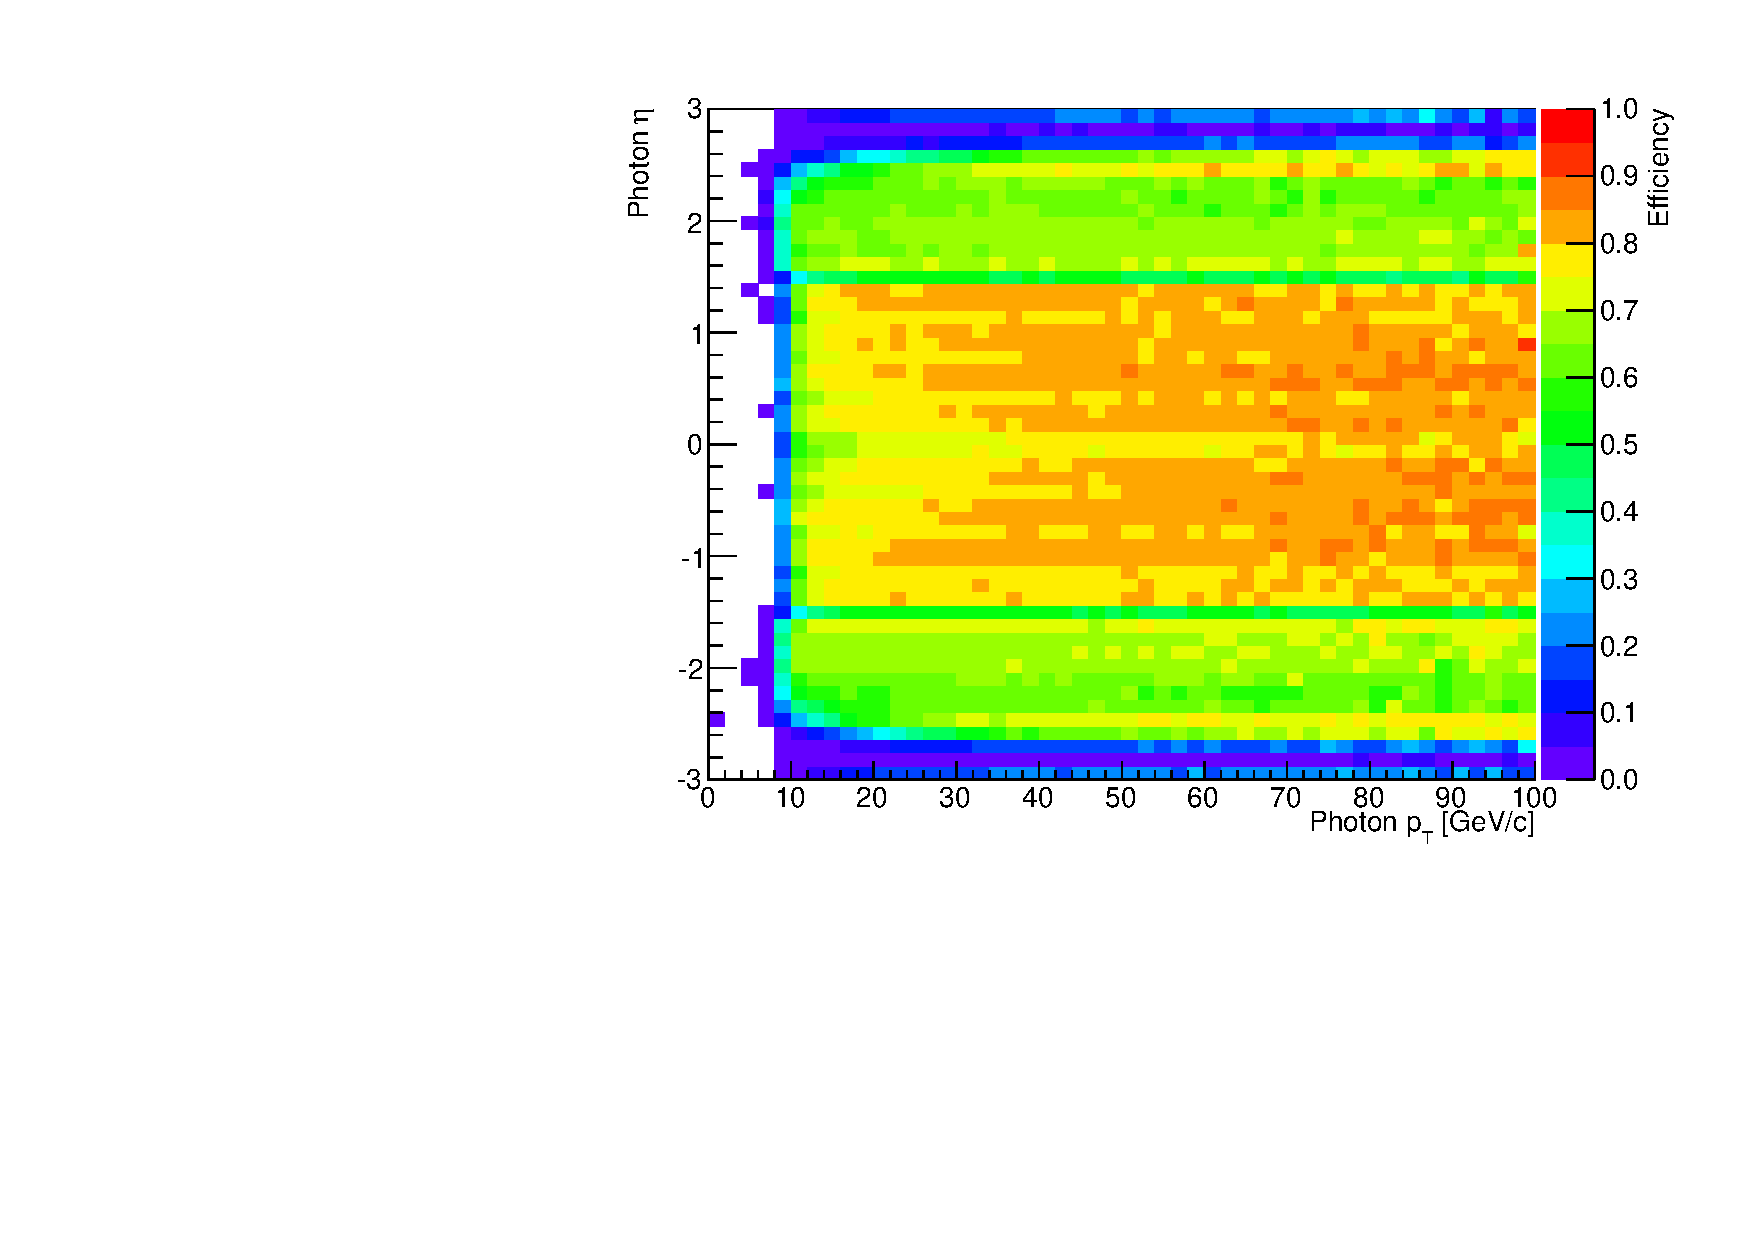
\includegraphics[width=0.9\textwidth]{figures/EfficiencyPtEta_PromptPhoton.pdf}
  \caption{Prompt Photon Selection Efficiency}
  \label{fig:photonEfficiency}
\end{figure}

\begin{figure}[h]
  \centering
  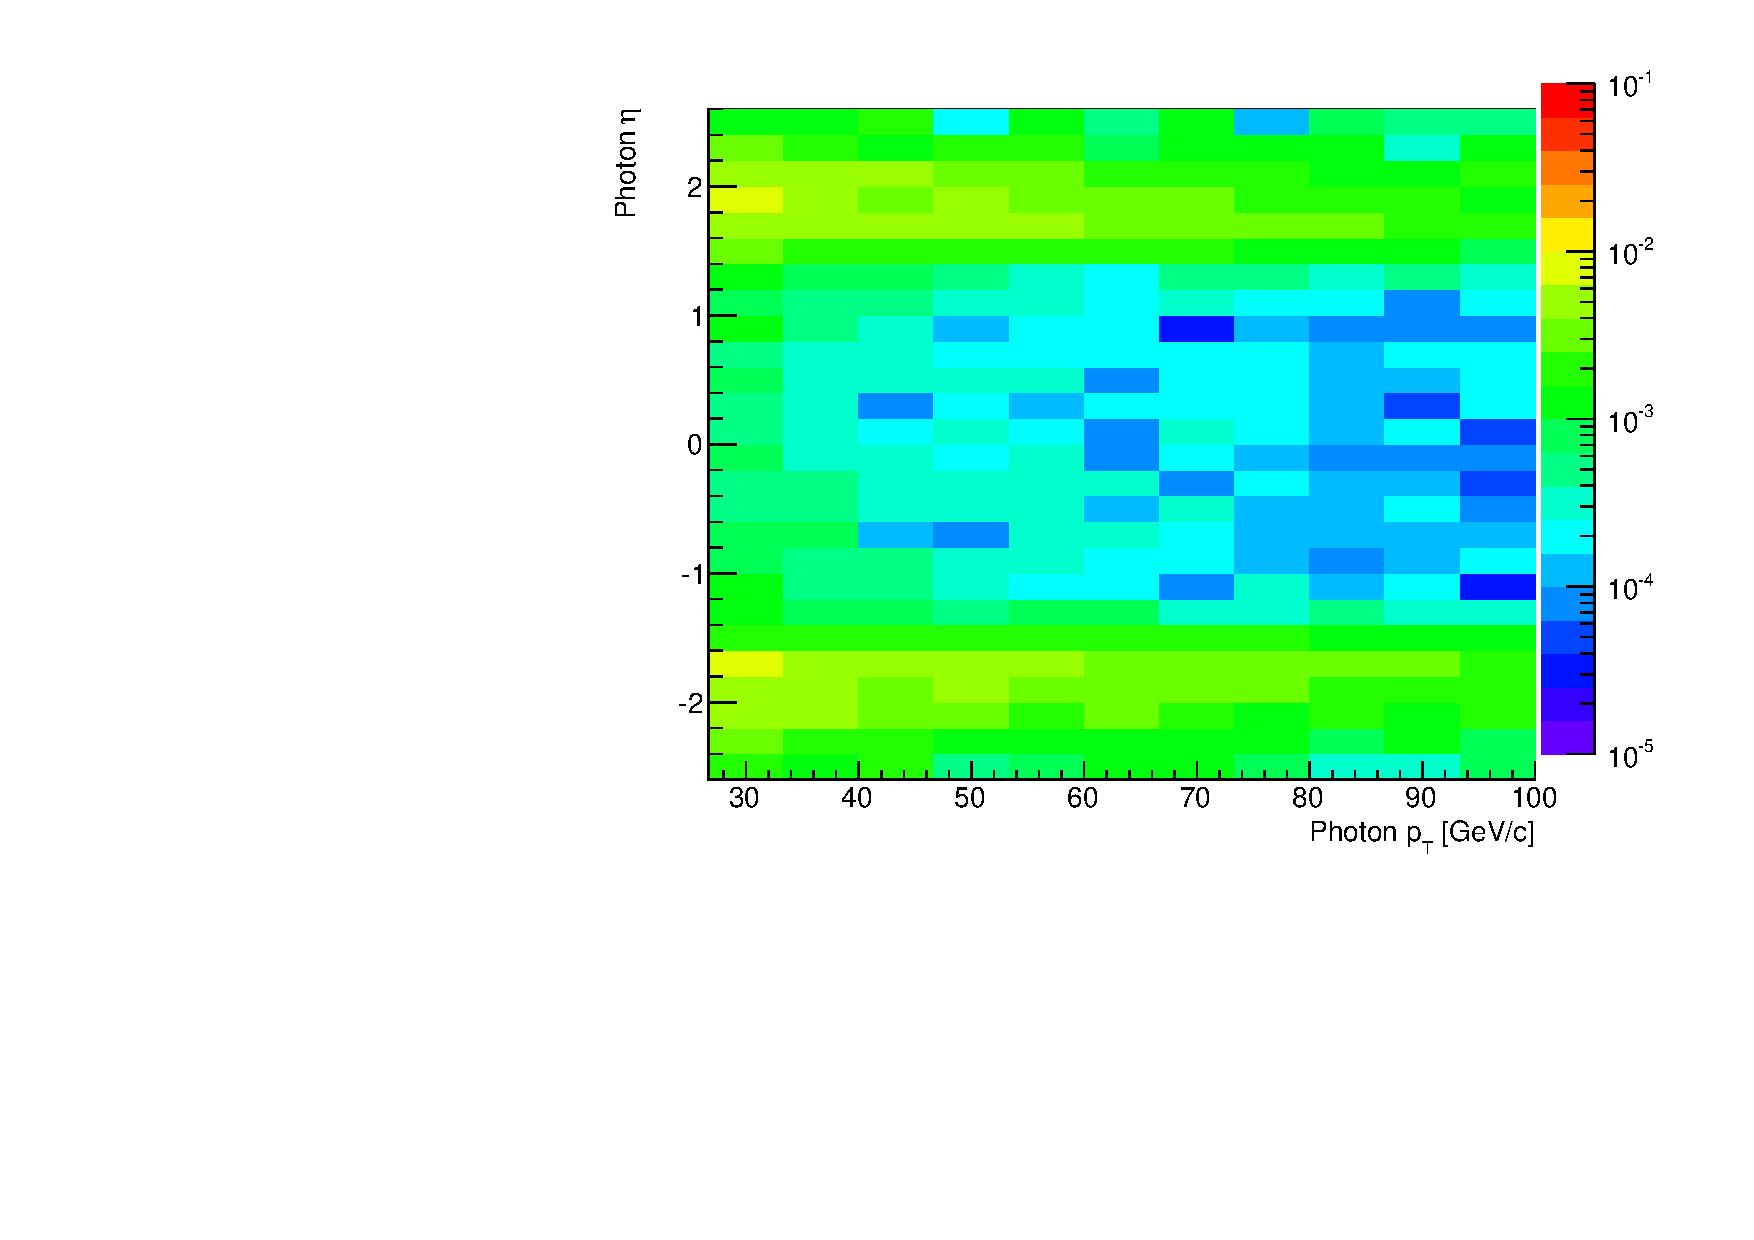
\includegraphics[width=0.45\textwidth]{figures/EfficiencyPtEta_GluonJetFakesPhoton.pdf}
  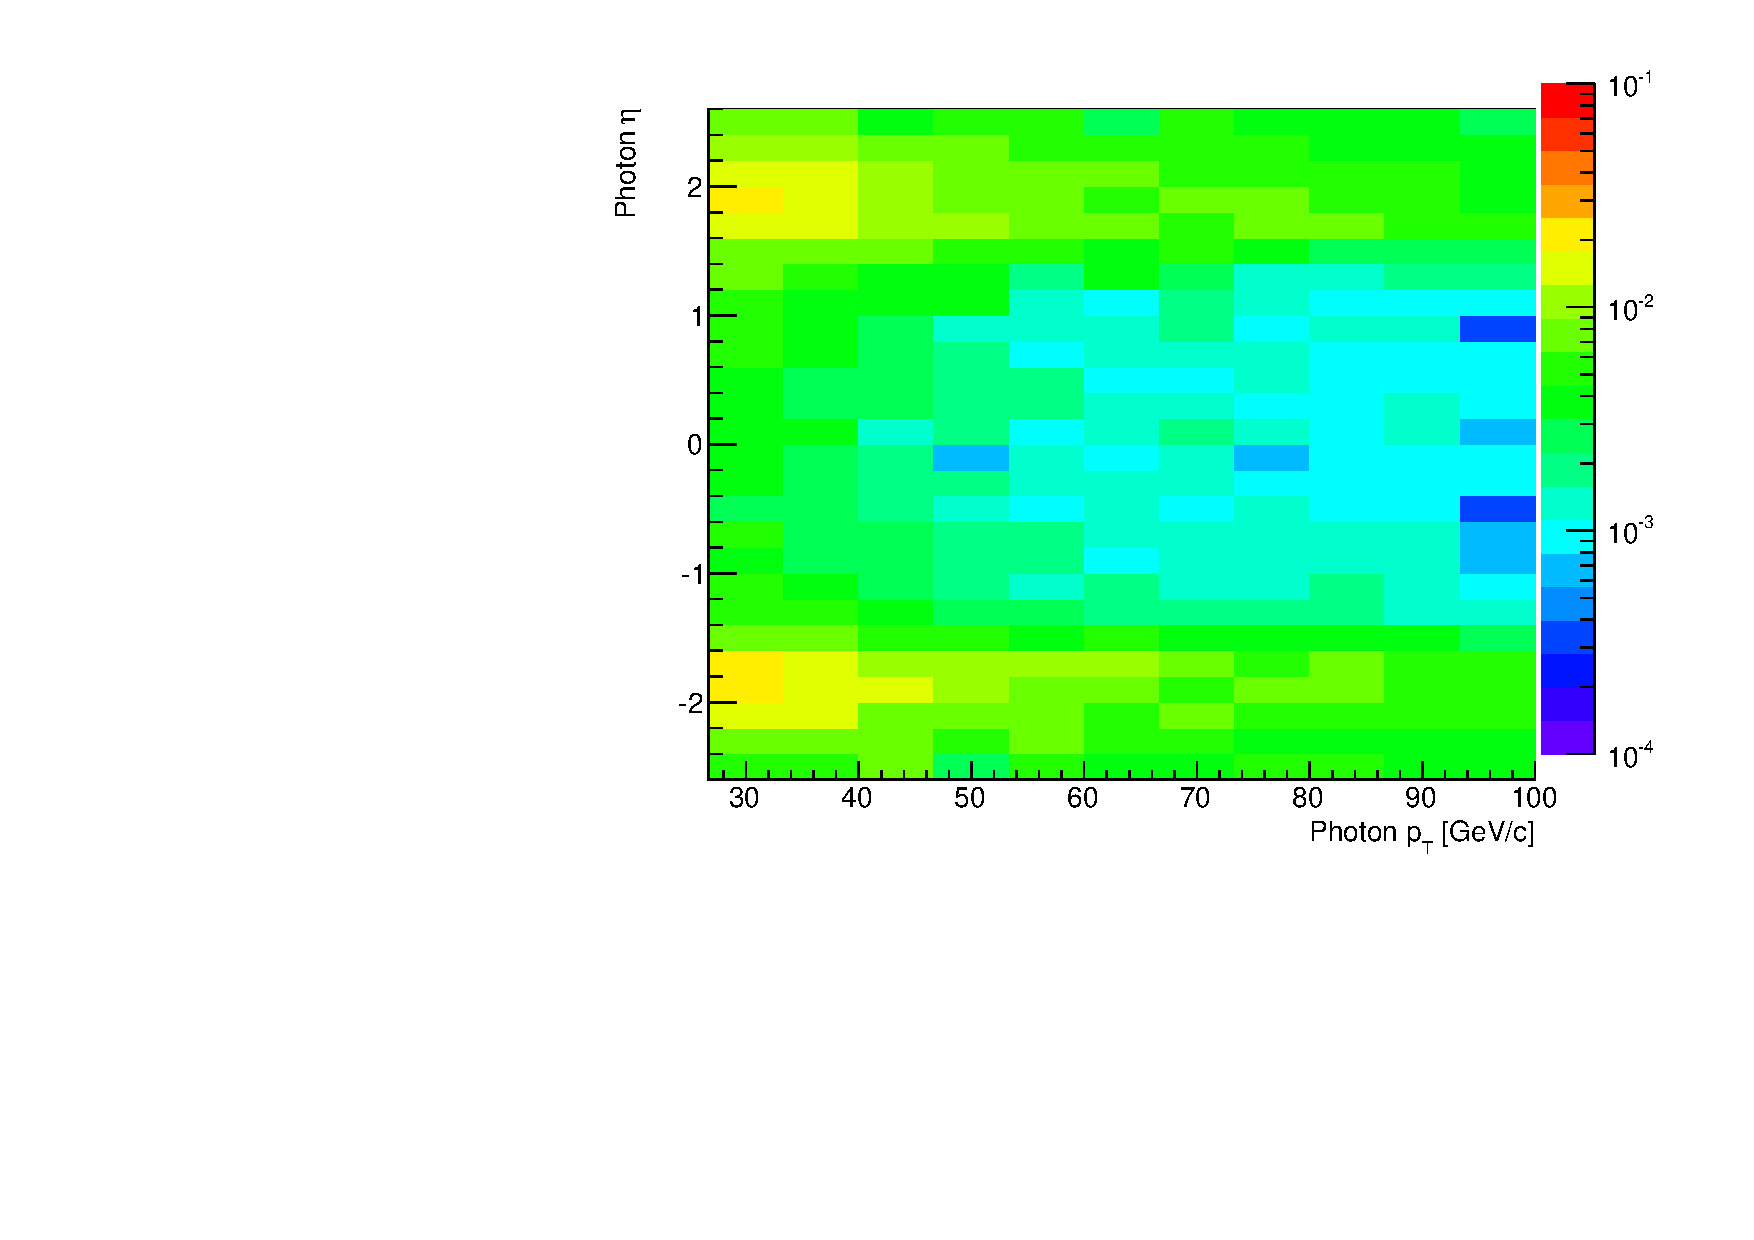
\includegraphics[width=0.45\textwidth]{figures/EfficiencyPtEta_QuarkJetFakesPhoton.pdf}
  \caption{Photon Fake Rate, left gluon jets, right quark jets.}
  \label{fig:photonFakeRate}
\end{figure}

Jets are reconstructed using the anti-Kt algorithm with the $D$ parameter equal to $0.5$,
and corrected for pileup effects using the FastJet technique \cite{CMS:2010xta,CMS-DP-2013-011}. Standard CMS 
jet energy corrections are applied up to level 3, correcting for non-uniformities as a function of
pseudorapditiy and $p_{T}$. Jets are tagged as originating from a b-quark by searching for the
presence of secondary vertices. Lifetime information from tracks are also combined to form a 
combined secondary vertex b-tagging discriminator (CSV)~\cite{CMS:BTagPaper,CMS-DP-2013-005}.
The medium working point for the CSV tagger is used. The efficiency for tagging b-jets is 
evaluated using full simulation of the current Run1 CMS detector and shown in
Figure \ref{fig:btagEfficiency}. On average, the b-tagging efficiency is about $70\%$ in the barrel, and
about $55\%$ in the endcap. The mistag rate for light jets and charm jets are also evaluated using
full simulation samples, and are shown in Figure \ref{fig:mistagRate}. The average mistag rate
for light jets is about $1\%$ and for charm jets is about $15\%$. 

\begin{figure}[h]
  \centering
  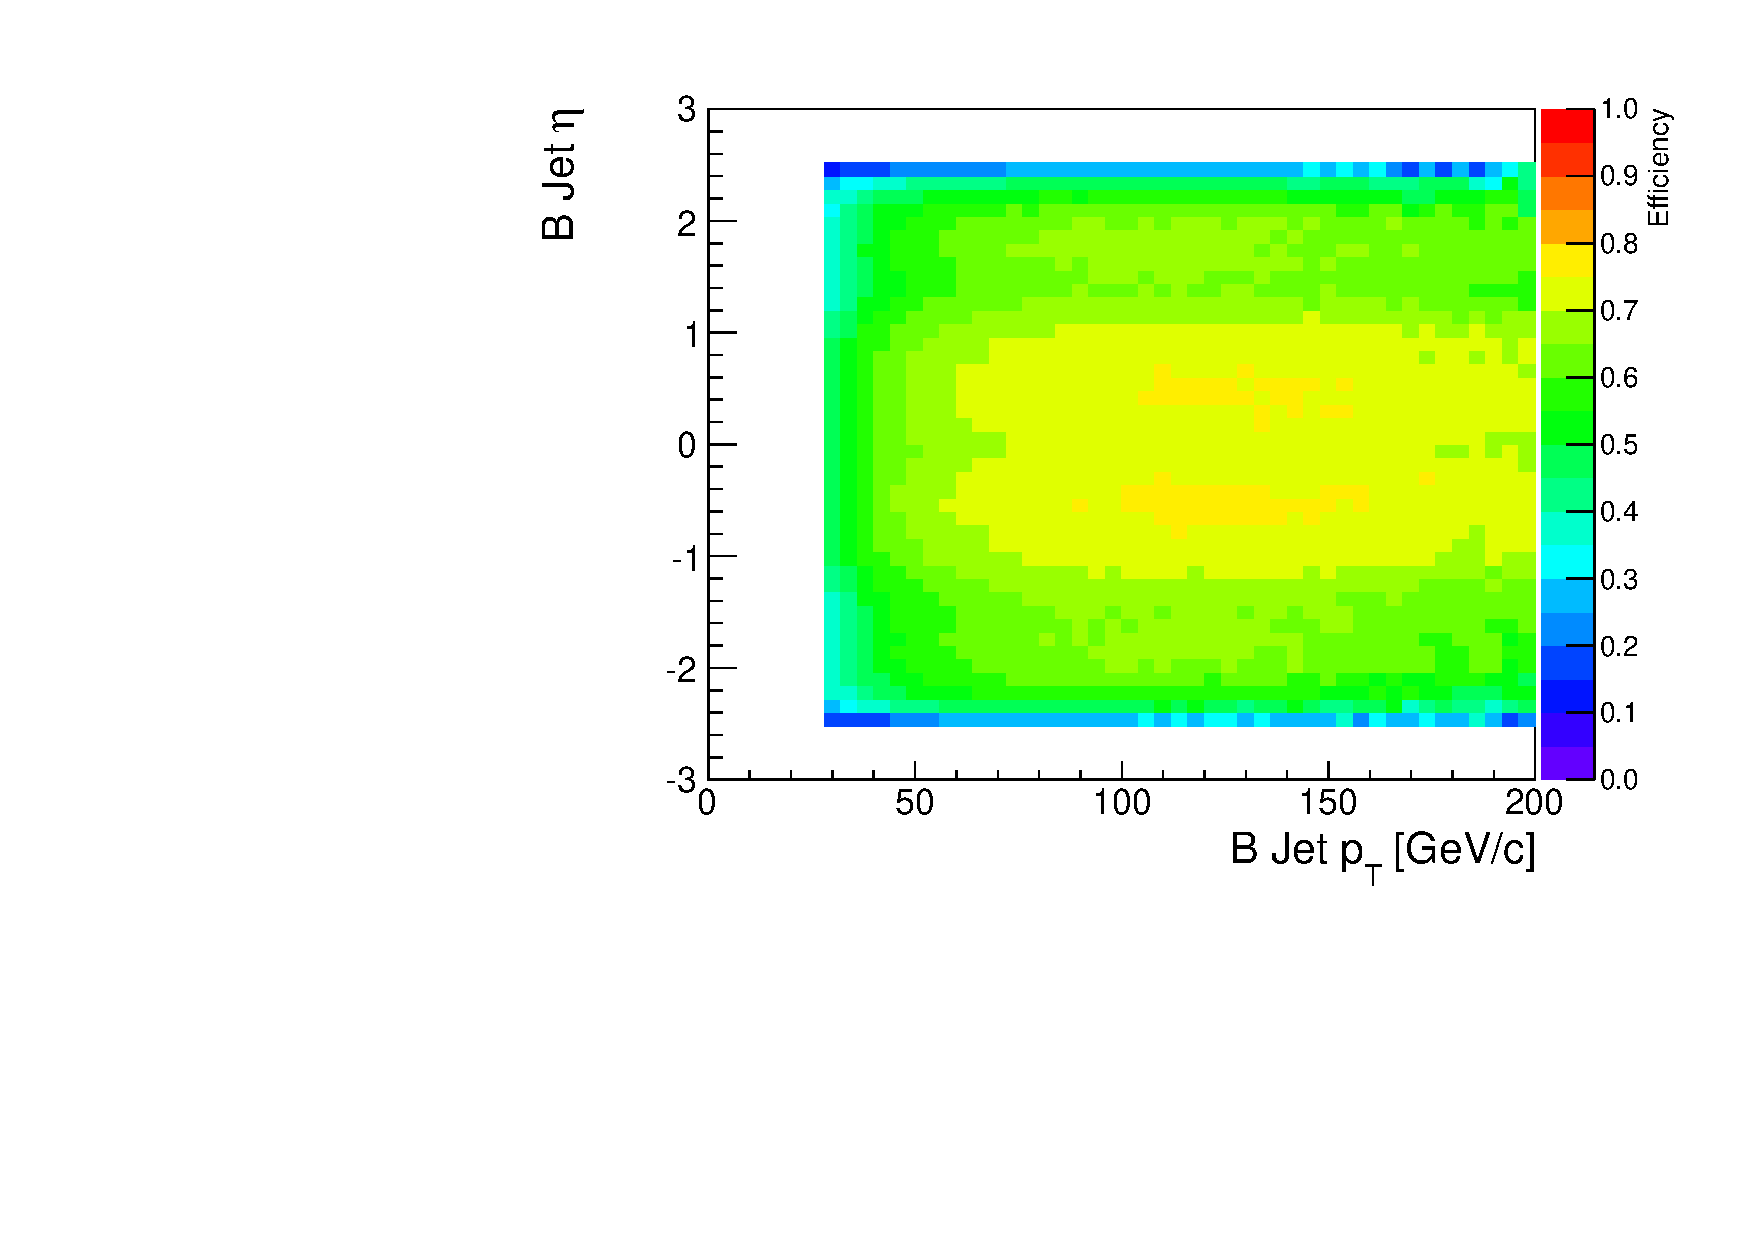
\includegraphics[width=0.9\textwidth]{figures/EfficiencyPtEta_BJet.pdf}
  \caption{BTag Efficiency}
  \label{fig:btagEfficiency}
\end{figure}

\begin{figure}[h]
  \centering
  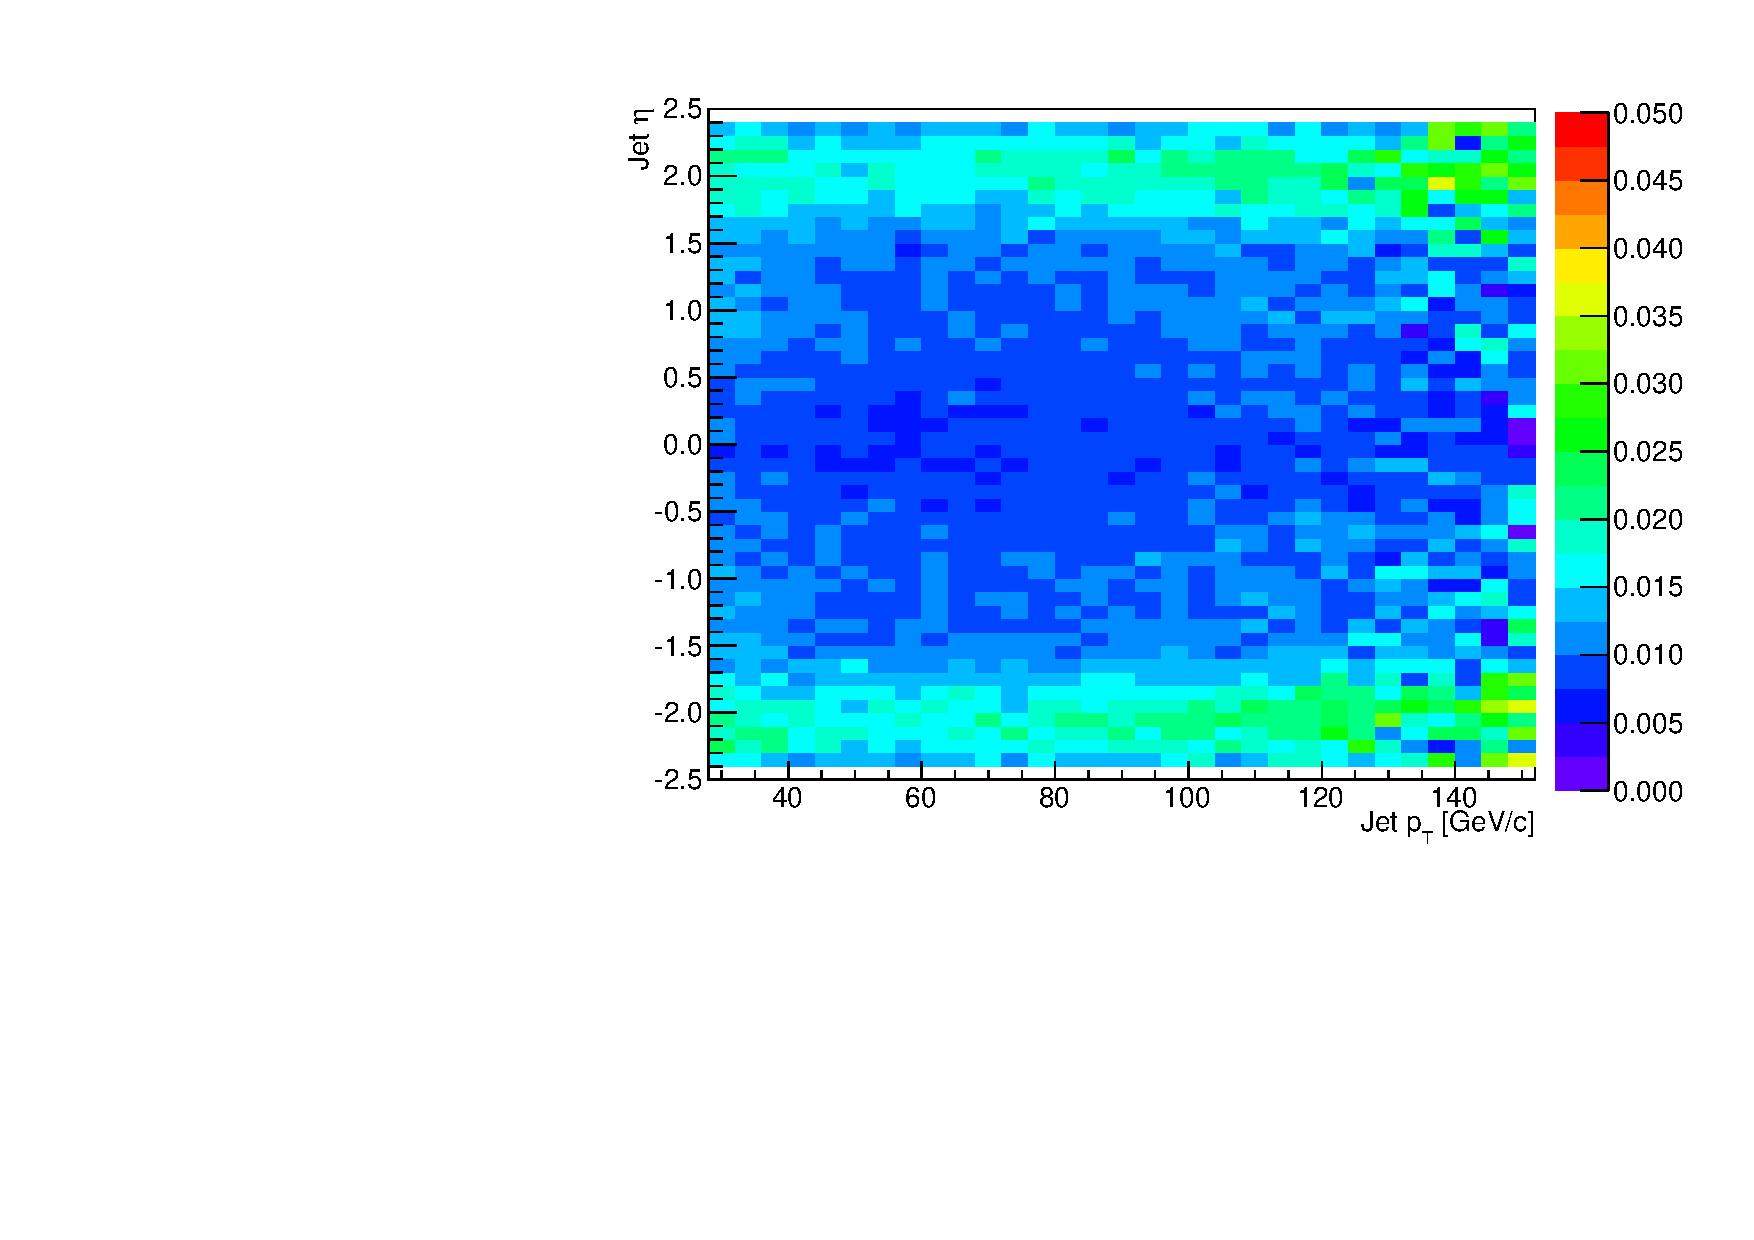
\includegraphics[width=0.45\textwidth]{figures/EfficiencyPtEta_LightJetMistag.pdf}
  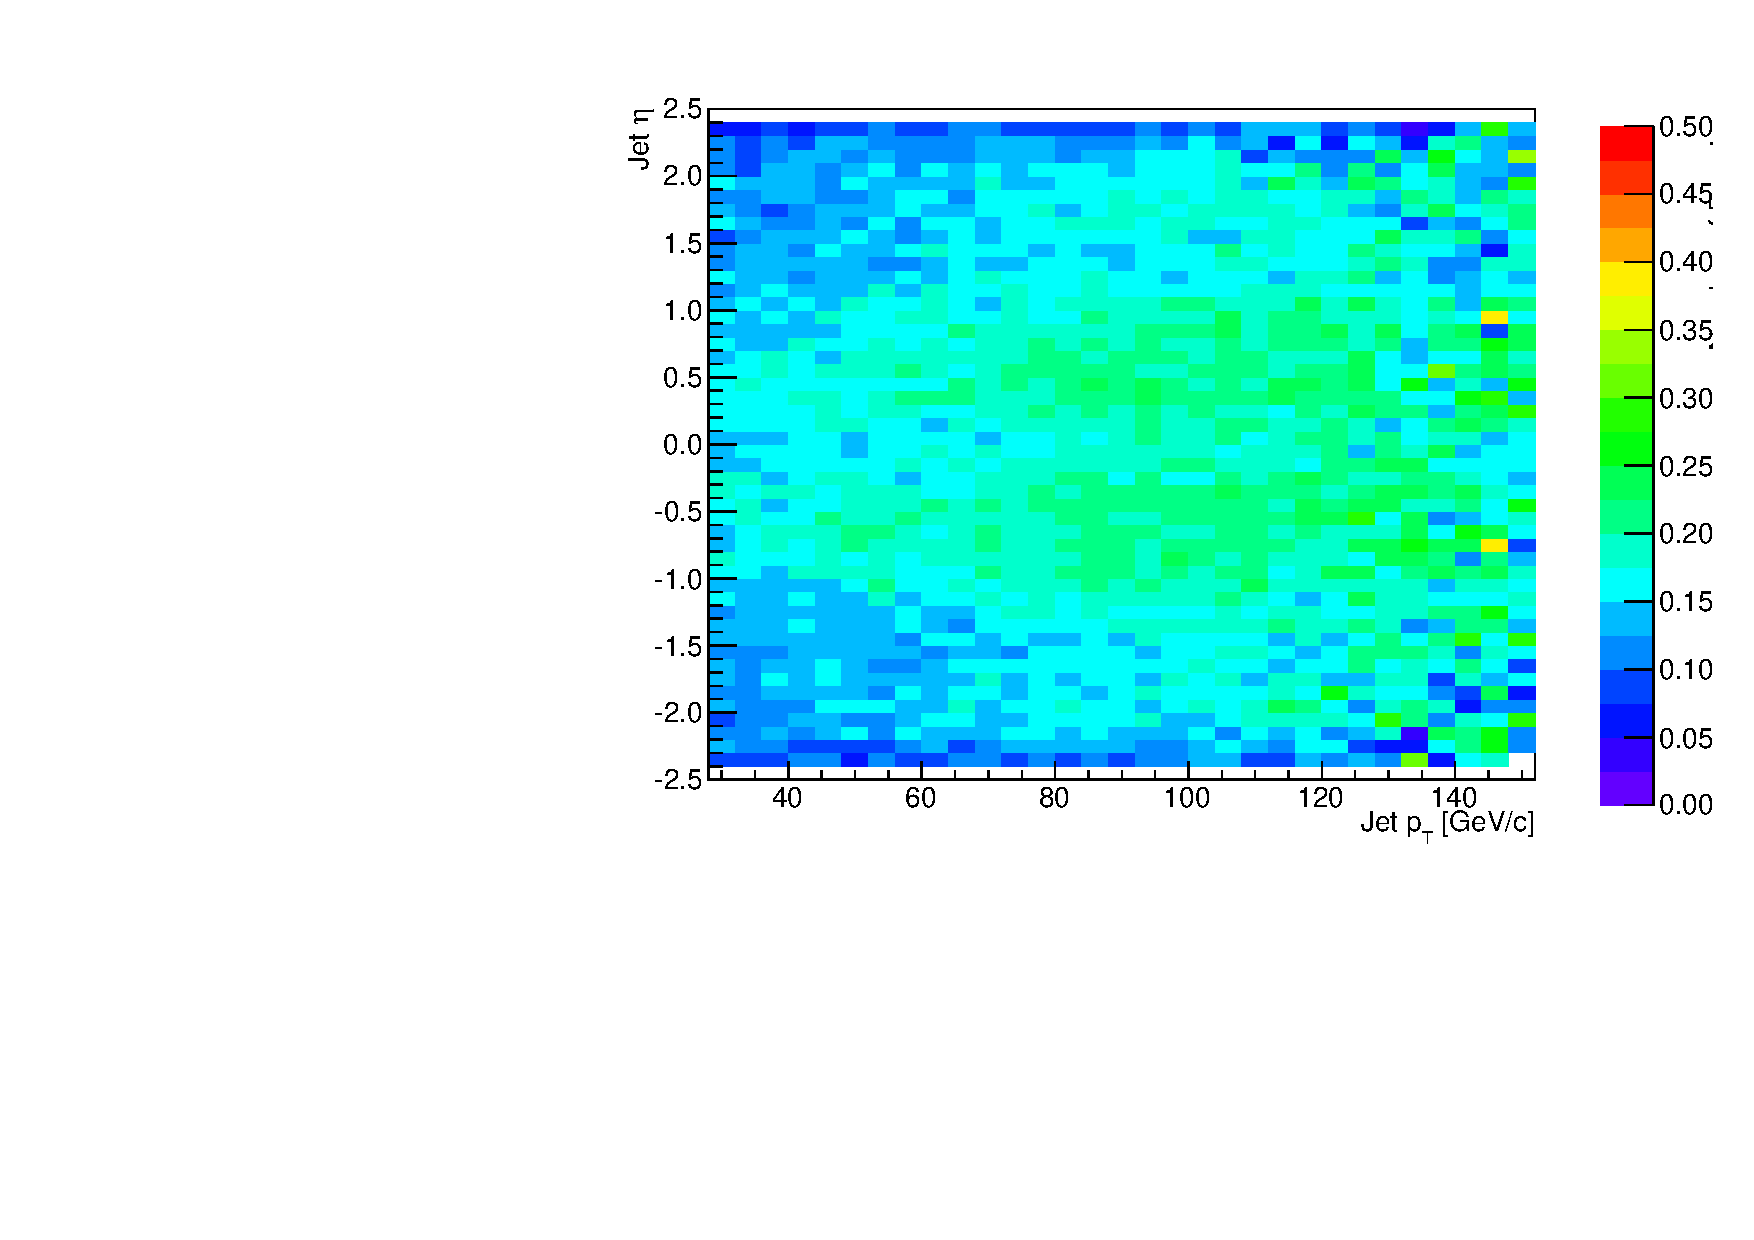
\includegraphics[width=0.45\textwidth]{figures/EfficiencyPtEta_CharmJetMistag.pdf}
  \caption{Mistag Rate, left light jets, right charm jets.}
  \label{fig:mistagRate}
\end{figure}


Electrons and Muons are selected for the purpose of vetoing events with signatures consistent
with Higgs produced in association with a top and anti top quark pair. This process contributes
significantly to the total background after signal event selection requirements. A non-negligble
fraction of such background events contain leptons and can be rejected on this basis. Very loose
selection requirements, denoted as the veto working point, are placed on the 
electron and muon candidates in order to suppress this background as much as possible. 

\subsection{Extrapolation to High Pileup}
\label{sec:HighPileupExtrapolation}

Using full simulation of the CMS Phase1 detector with an average of 140 pileup events, we extrapolate
the photon and b-tagging efficiency and the photon fake rates and mistag rates to pileup conditions
expected for the high luminosity LHC. 

Figures \ref{} and ref{} show the efficiency for b-tagging and the mistag rate for light jets 
as a function of the number of pileup events mixed with the primary interaction. Based on these efficiencies, 
to extrapolate to conditions corresponding to an average of 140 pileup events we decrease
the b-tagging efficiency by $XX\%$ and increase the mistag rate by a factor of $X$. 

%More on photons



\section{Event Selection and Optimization}
\label{sec:eventselection}
 
We begin by selecting events containing two photons with $p_{T}$ greater than $25$~GeV
and $|\eta|<2.5$, and two b-tagged jets with $p_{T}$ greater than $30$~GeV and $|\eta|<2.4$.
One of the two photons is required to have $p_{T} > 40$~GeV. To suppress $t\bar{t}H$ background
events, we require that there are no electrons or muons passing the veto selection and that 
the number of jets with $|\eta|<2.5$ is less than $4$. In Figure~\ref{fig:LeptonVetoAndJetCounting}, 
we show the distribution of the number of selected leptons and the number of jets with $|\eta|<2.5$ 
for the di-Higgs signal and the $t\bar{t}H$ background
to demonstrate the effectiveness of the lepton veto and jet counting requirements.

\begin{figure}[h]
\centering
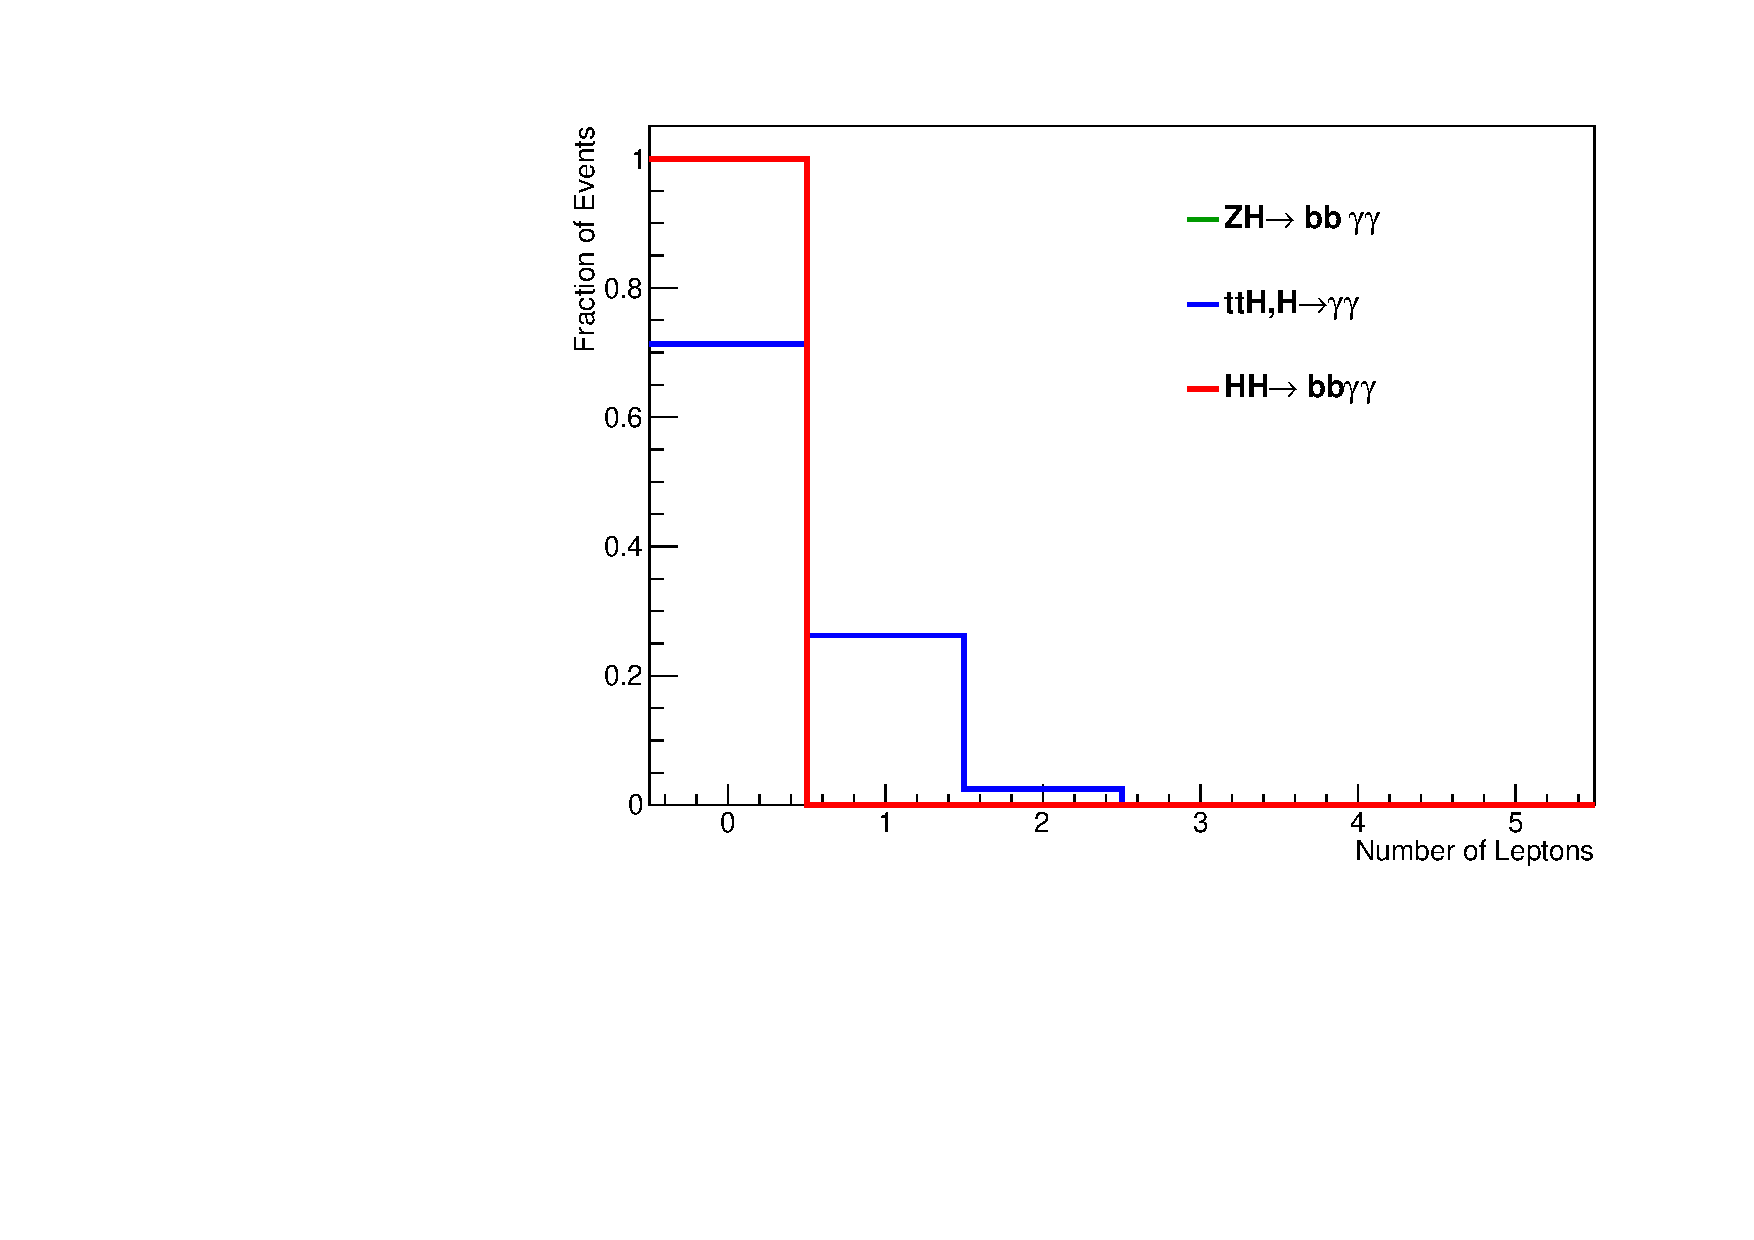
\includegraphics[width=0.48\textwidth]{figures/NLeptons.pdf}	
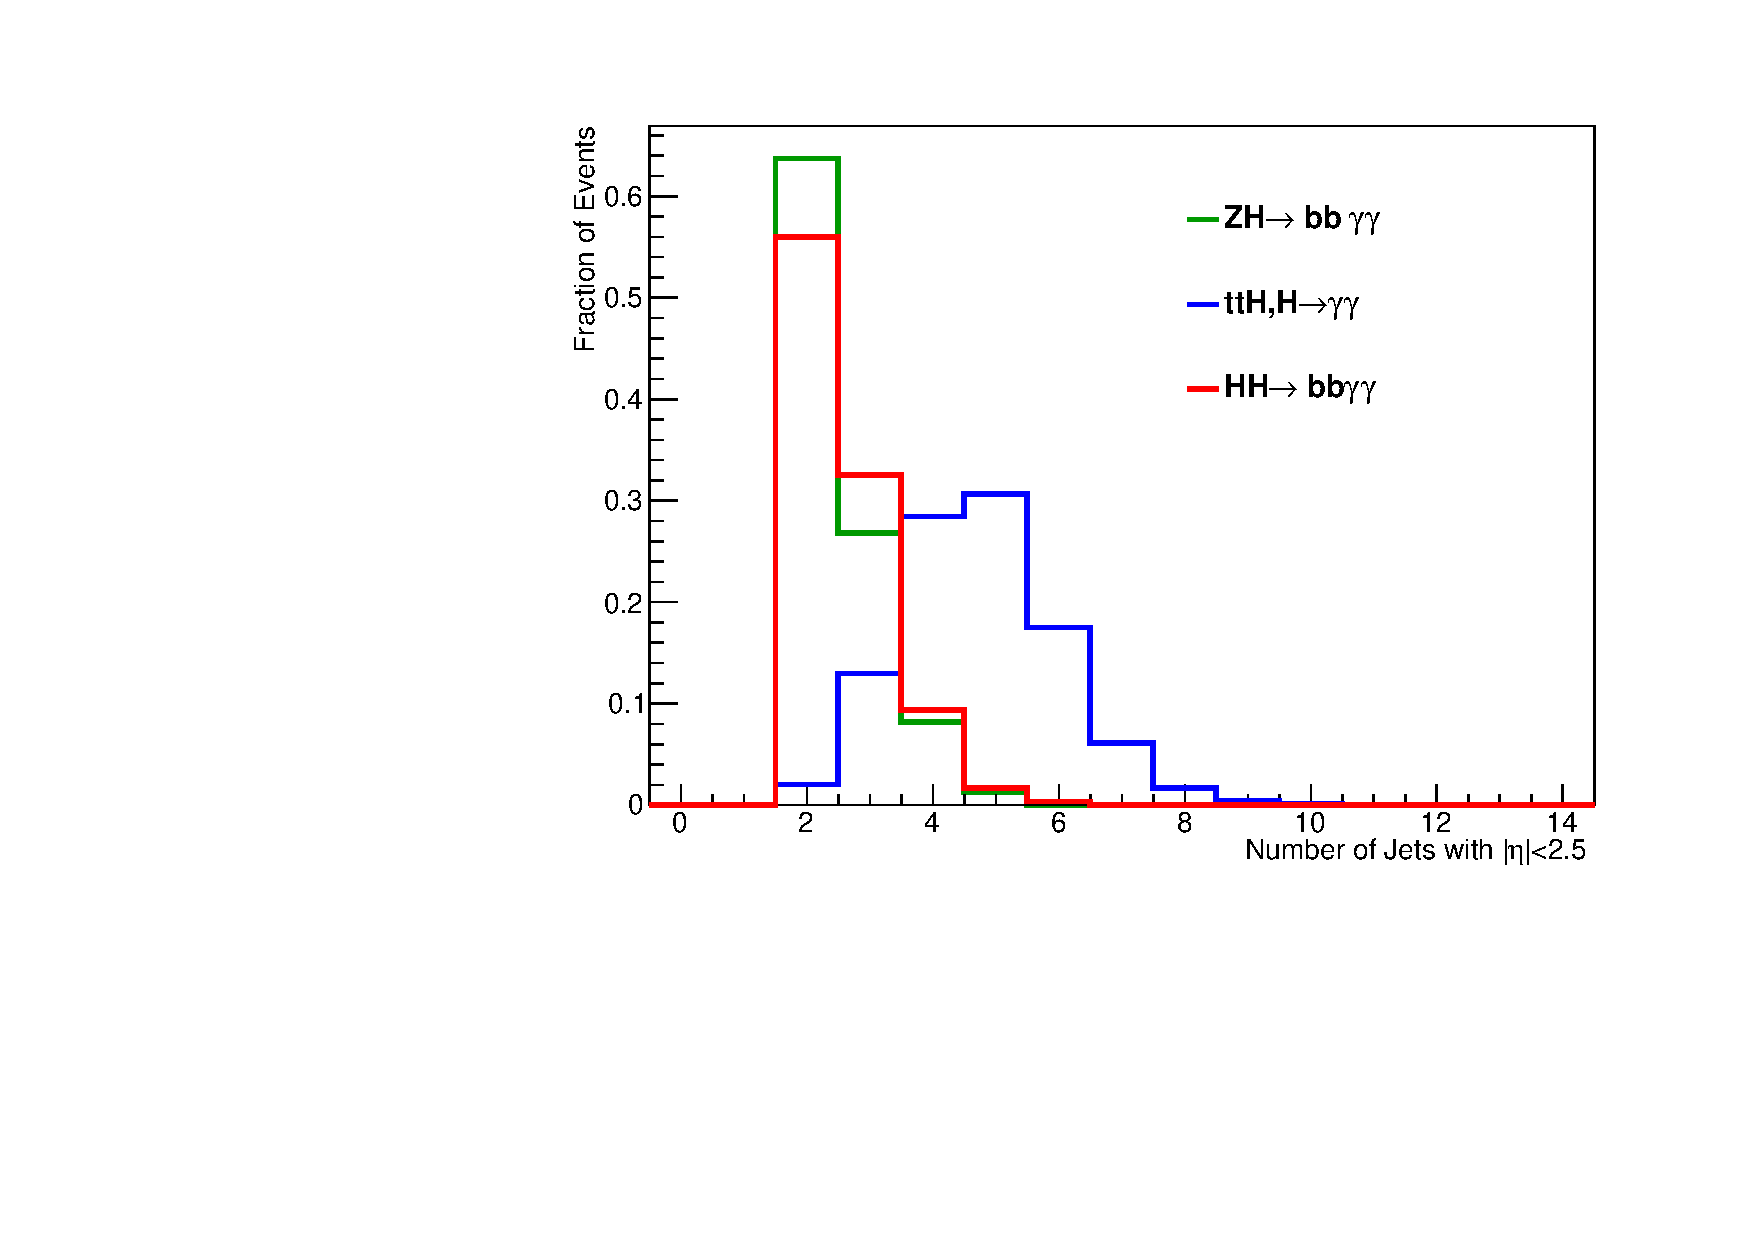
\includegraphics[width=0.48\textwidth]{figures/Ncentraljets.pdf}	
\caption{Distributions of the number of selected leptons and the number of jets with $|\eta|<2.5$ for 
the di-Higgs signal, the $t\bar{t}H$ background, and the ZH background, are shown normalized in area.}
\label{fig:LeptonVetoAndJetCounting}
\end{figure}

We investigated a number of different additional kinematic requirements in order to improve the
signal to background ratio. Following the motivation from the ATLAS public note \cite{ATLASHHToBBGG},
we apply requirements on the $\Delta$R between the two photons, and the minimum of the 
$\Delta R$ between photons and b-jets. We denote these selection requirements as ``Scheme 0'', 
requiring that $\Delta R_{\gamma\gamma}<2.0$ and $min\Delta R_{\gamma b}>1.0$. 
In Figure \ref{fig:scheme0}, we show the distributions for $\Delta R_{\gamma\gamma}$ and $min\Delta R_{\gamma b}$ 
after the object selection cuts to illustrate the effectiveness of these angular requirements.

\begin{figure}[h]
\centering
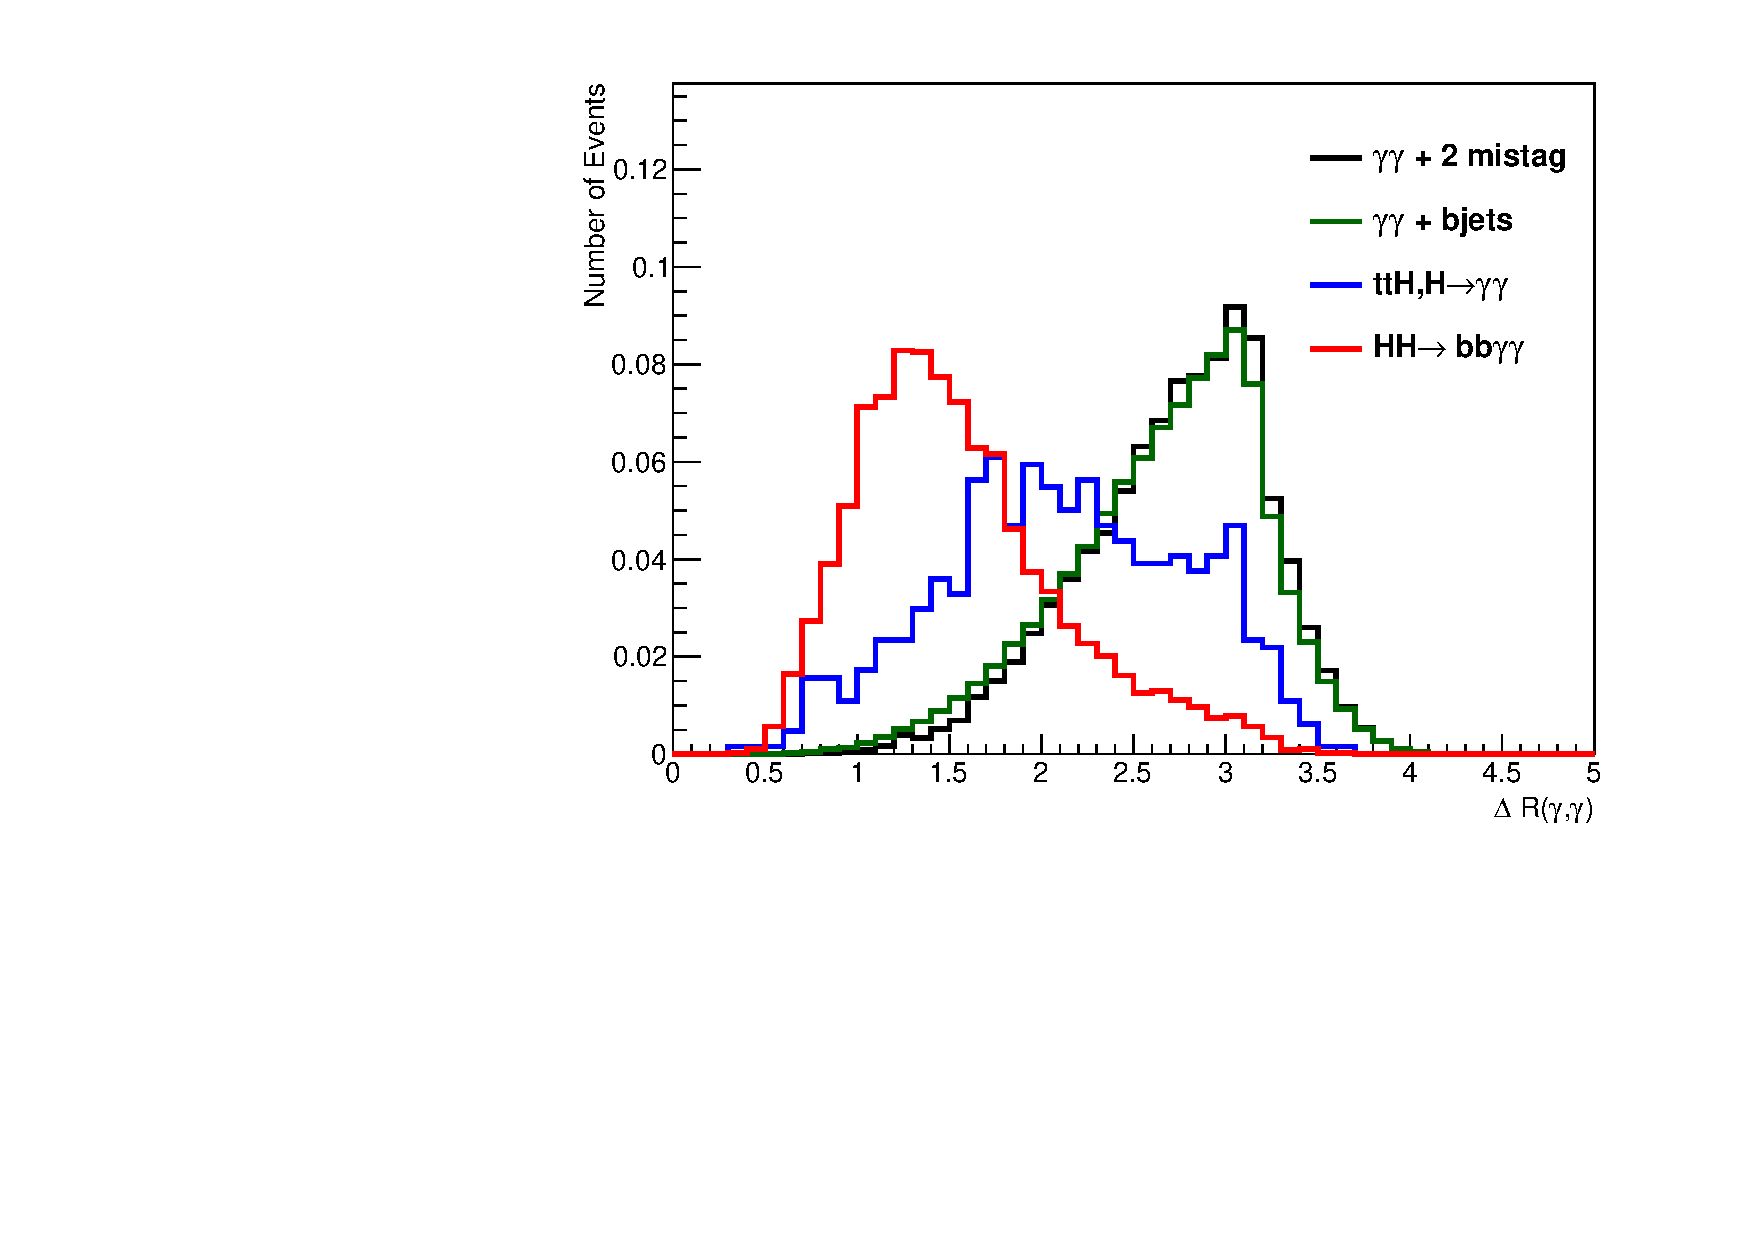
\includegraphics[scale=0.38, angle=0]{figures/Cuts/dRgg_ps_normalized}	
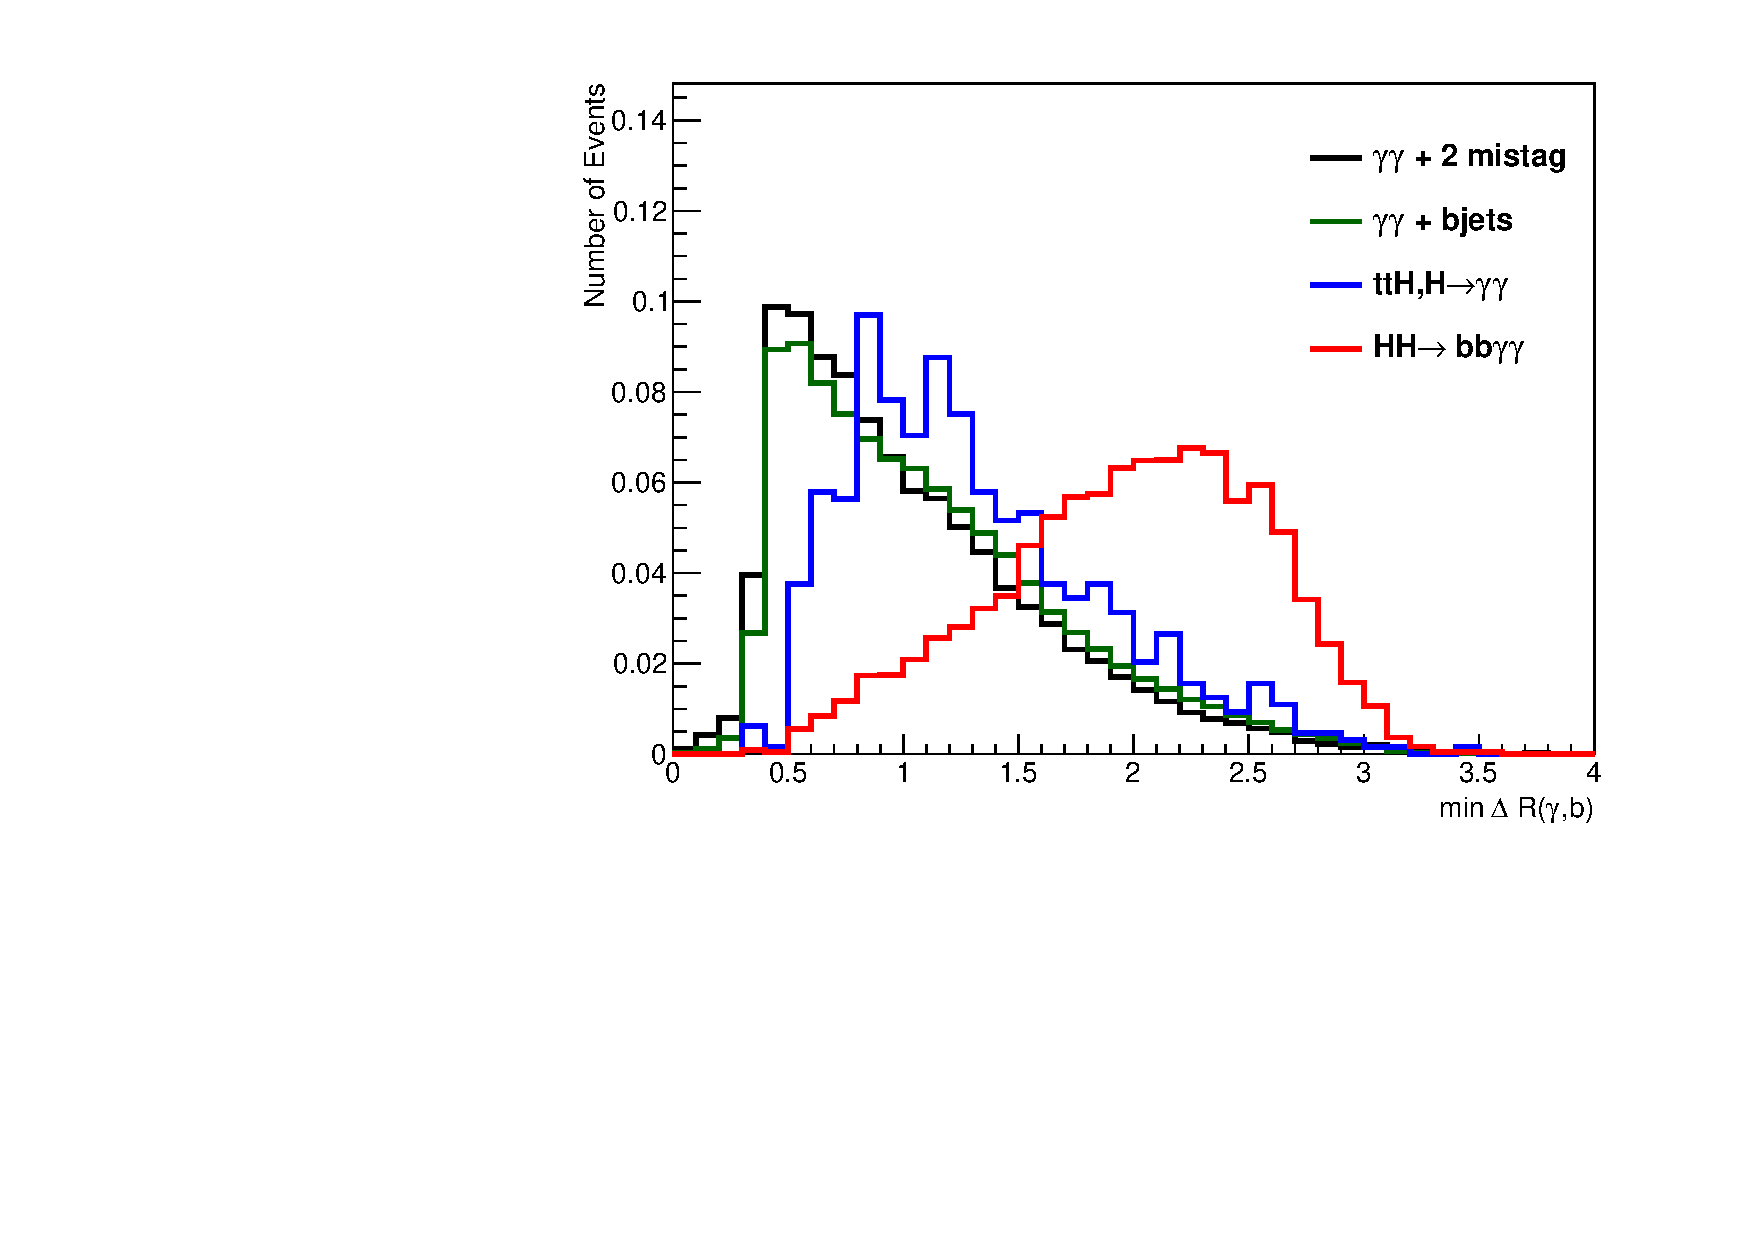
\includegraphics[scale=0.38, angle=0]{figures/Cuts/minDRgb_ps_normalized.pdf}	
\caption{Distributions of $\Delta R_{\gamma\gamma}$ and $min\Delta R_{\gamma b}$ are shown for the 
di-Higgs signal, the  $t\bar{t}H$ background, and the QCD non-resonant backgrounds, and are
normalized in area. }
\label{fig:scheme0}
\end{figure}

We examined additional requirements for further signal to background optimization. 
We tighten the requirement on the minimum of the $\Delta$R between photons and b-jets, 
requiring that  $min\Delta R_{\gamma b} > 1.5$, and we add a requirement on
the $\Delta$R between the two b-jets: $\Delta R_{b\bar{b}}<2.0$. These cuts in addition
to the cuts used above are denoted as ``Scheme 1'' selection. 
In Figure \ref{fig:dRbb_s0}, we show $\Delta R_{b\bar{b}}$ after the ``Scheme 0'' cuts 
to demonstrate the effectiveness of this additional requirement in reducing background, while
retaining the majority of the signal events. 

\begin{figure}
\centering
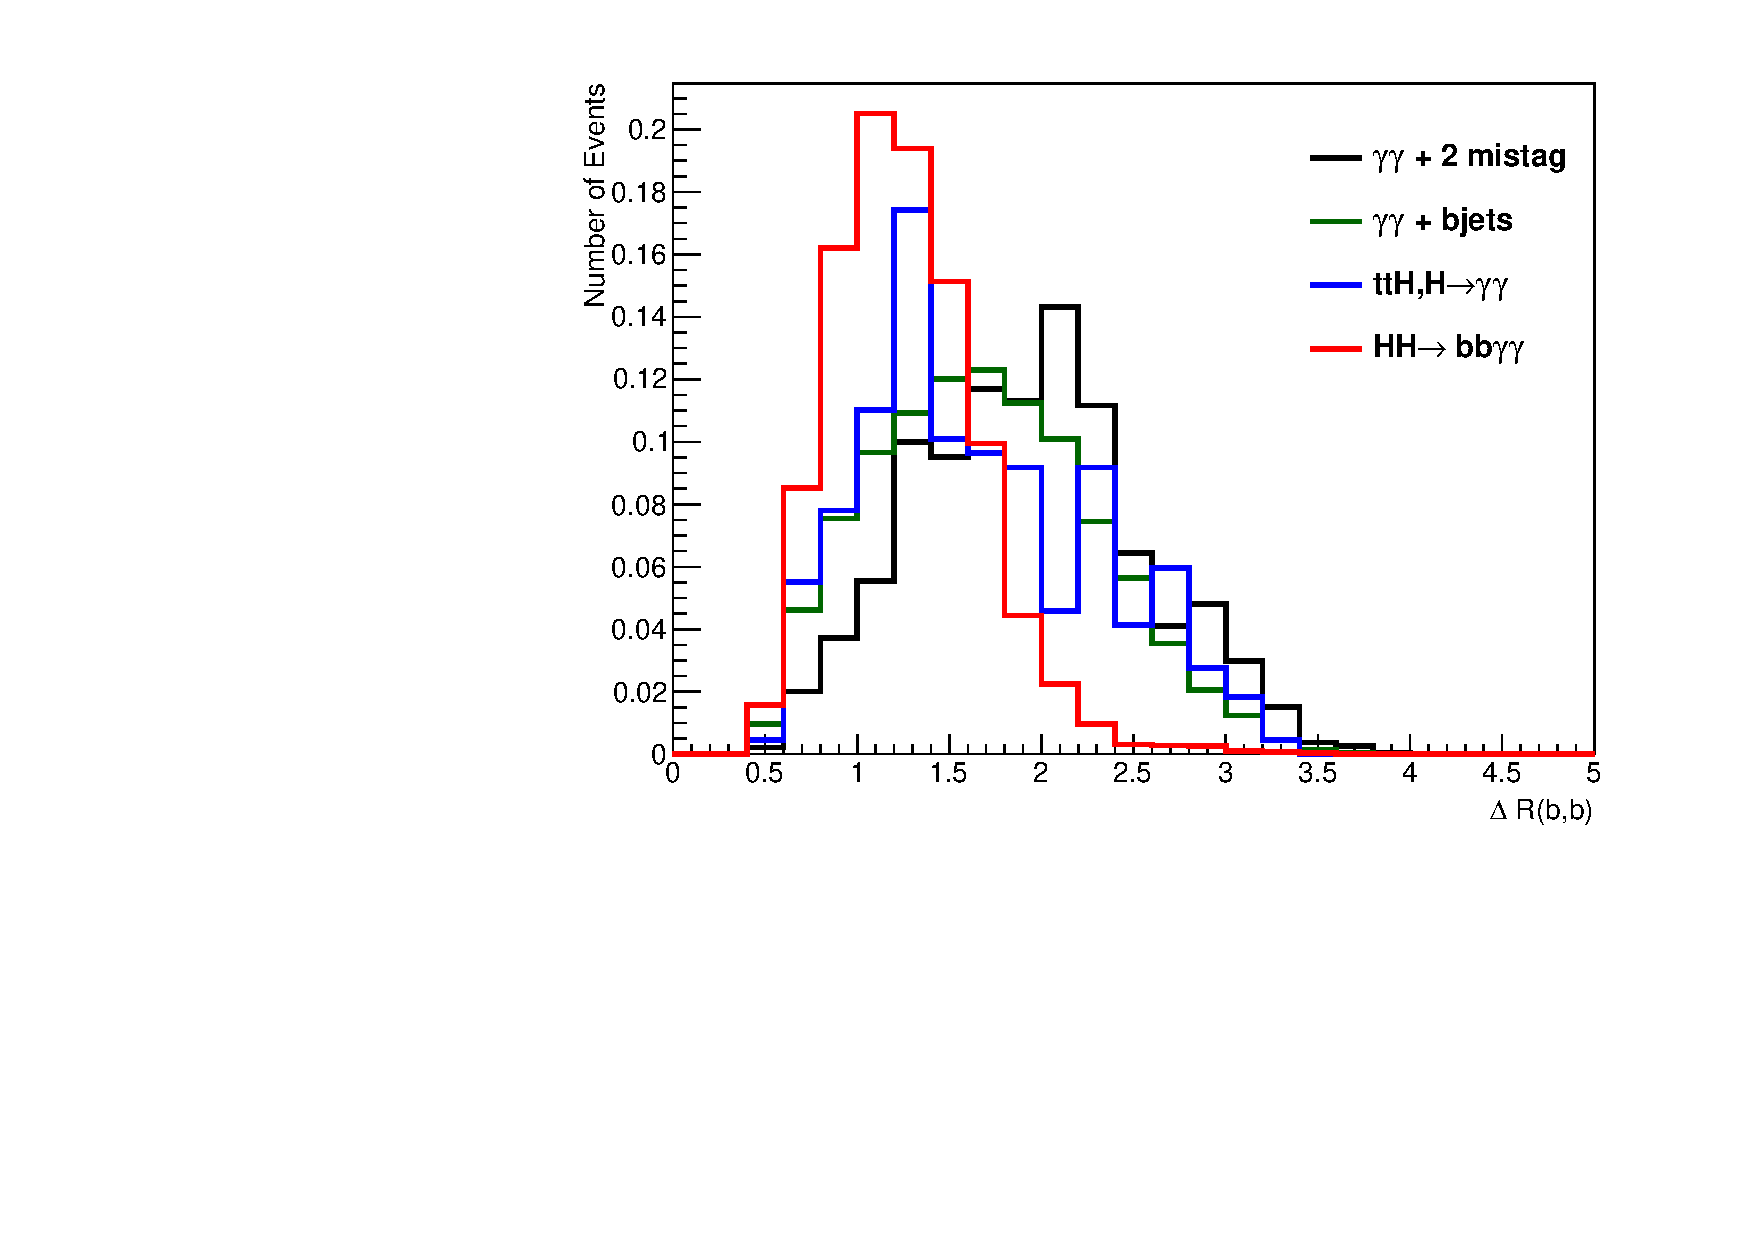
\includegraphics[scale=0.45, angle=0]{figures/Cuts/dRbb_s0_normalized.pdf}	
\caption{dRbb after Scheme 0 cuts}
\label{fig:dRbb_s0}
\end{figure}

In Table \ref{tab:scheme1_events}, we summarize the expected event yields for the signal and 
various background processes for an integrated luminosity of $3000$~$pb^{-1}$ after 
the ``Scheme 1'' selection requirements. The methods used to estimate the backgrounds
are described in greater detail in Section \ref{sec:bkgestimation}. The event yields
for three different mass windows are provided corresponding to the mass windows
used for the mass fit analysis described later in Section \ref{sec:massfits}, a mass window
corresponding to a conservative estimate of the expected mass resolutions, 
and a mass window corresponding to a more optimistic estimate of the expected mass resolution.
\begin{table}[!ht]
\begin{center}
\begin{tabular}{|c|c|c|c|c|}
\hline
\multicolumn{4}{|c|}{\textbf{Expected Event Yield: Scheme 1 Selection}}                                 \\ \hline
Sample Type & Fit Window                    & Conservative Window           & More Optimistic Window    \\ 
            & $M_{b\bar{b}}:$ (70,200)      & $M_{b\bar{b}}$: (105,145)     & $M_{b\bar{b}}$: (110,140)      \\ 
            & $M_{\gamma\gamma}$: (100,150) & $M_{\gamma\gamma}$: (120,130) & $M_{\gamma\gamma}$: (122,128)  \\ 
\hline
$HH\rightarrow bb\gamma\gamma$     & 16.3     & 12.0     & 9.4       \\ \hline
$ZH\rightarrow bb \gamma\gamma$    & 19.4     & 2.9      & 1.3       \\ 
$ttH,H\rightarrow\gamma\gamma$     & 4.8      & 1.7      & 1.2       \\ 
$bb\gamma\gamma$                   & 150.4    & 9.6      & 4.5       \\ 
$jj\gamma\gamma$                   & 114.5    & 8.0      & 4.1       \\ 
$jjjj$, $ccjj$, $bbjj$             & 11.1     & 0.0      & 0.0       \\ 
$t\bar{t}$                         & 5.3      & 0.2      & 0.0       \\ \hline
S/B Ratio                          & 0.1      & 0.5      & 0.8       \\ \hline
$S/\sqrt{B}$ (Signal Significance) & 0.9      & 2.5      & 2.8       \\ \hline
\end{tabular}
\caption{Scheme 1 expected events}
\label{tab:scheme1_events}
\end{center}
\end{table}

Furthermore, we studied an alternative kinematic selection scheme, where cuts are applied
on the transverse momenta of the diphoton, di-bjet, and di-Higgs systems rather than the angular variables.
The distributions of these transverse momentum observables are shown in Figure \ref{fig:Ptcuts} for the 
di-Higgs signal, the  $t\bar{t}H$ background, and the QCD non-resonant backgrounds, after objection
selection but before any other kinematic cuts are applied. We introduce the ``Scheme 2'' 
kinematic selection requirements where we require that $10 < P_{Tb\bar{b}\gamma\gamma} < 110$ $GeV/c$ 
and $(P_{Tb\bar{b}}+P_{T\gamma\gamma})>260$ $GeV/c$. 
Finally, we introduce the ``Scheme 1 Tight'' selection by further tightening the 
cuts on the angular variables, requiring that $\Delta R_{\gamma\gamma} < 1.6$, 
$\Delta R_{b\bar{b}}<1.6$ and $min\Delta R_{\gamma b} > 1.5$. 

In Table \ref{tab:event_schemes}, we compare the expected signal and background event yields
within the conservative mass window defined above for the four selection schemes that we studied. 
We observe that ``Scheme1'' and ``Scheme2'' achieve similar signal to background ratios, and both
improve slightly upon the ``Scheme0'' selection. The ``Scheme 1 Tight'' selection achieves
significantly improves signal to background, but at a cost of about $25\%$ in signal efficiency.
Attempts at achieving better signal to background ratio by tightening cuts in the ``Scheme 2''
scenario resulted in significantly larger reduction in signal yield compared to the ``Scheme 1 tight''
scenario. 

\begin{figure}
\centering
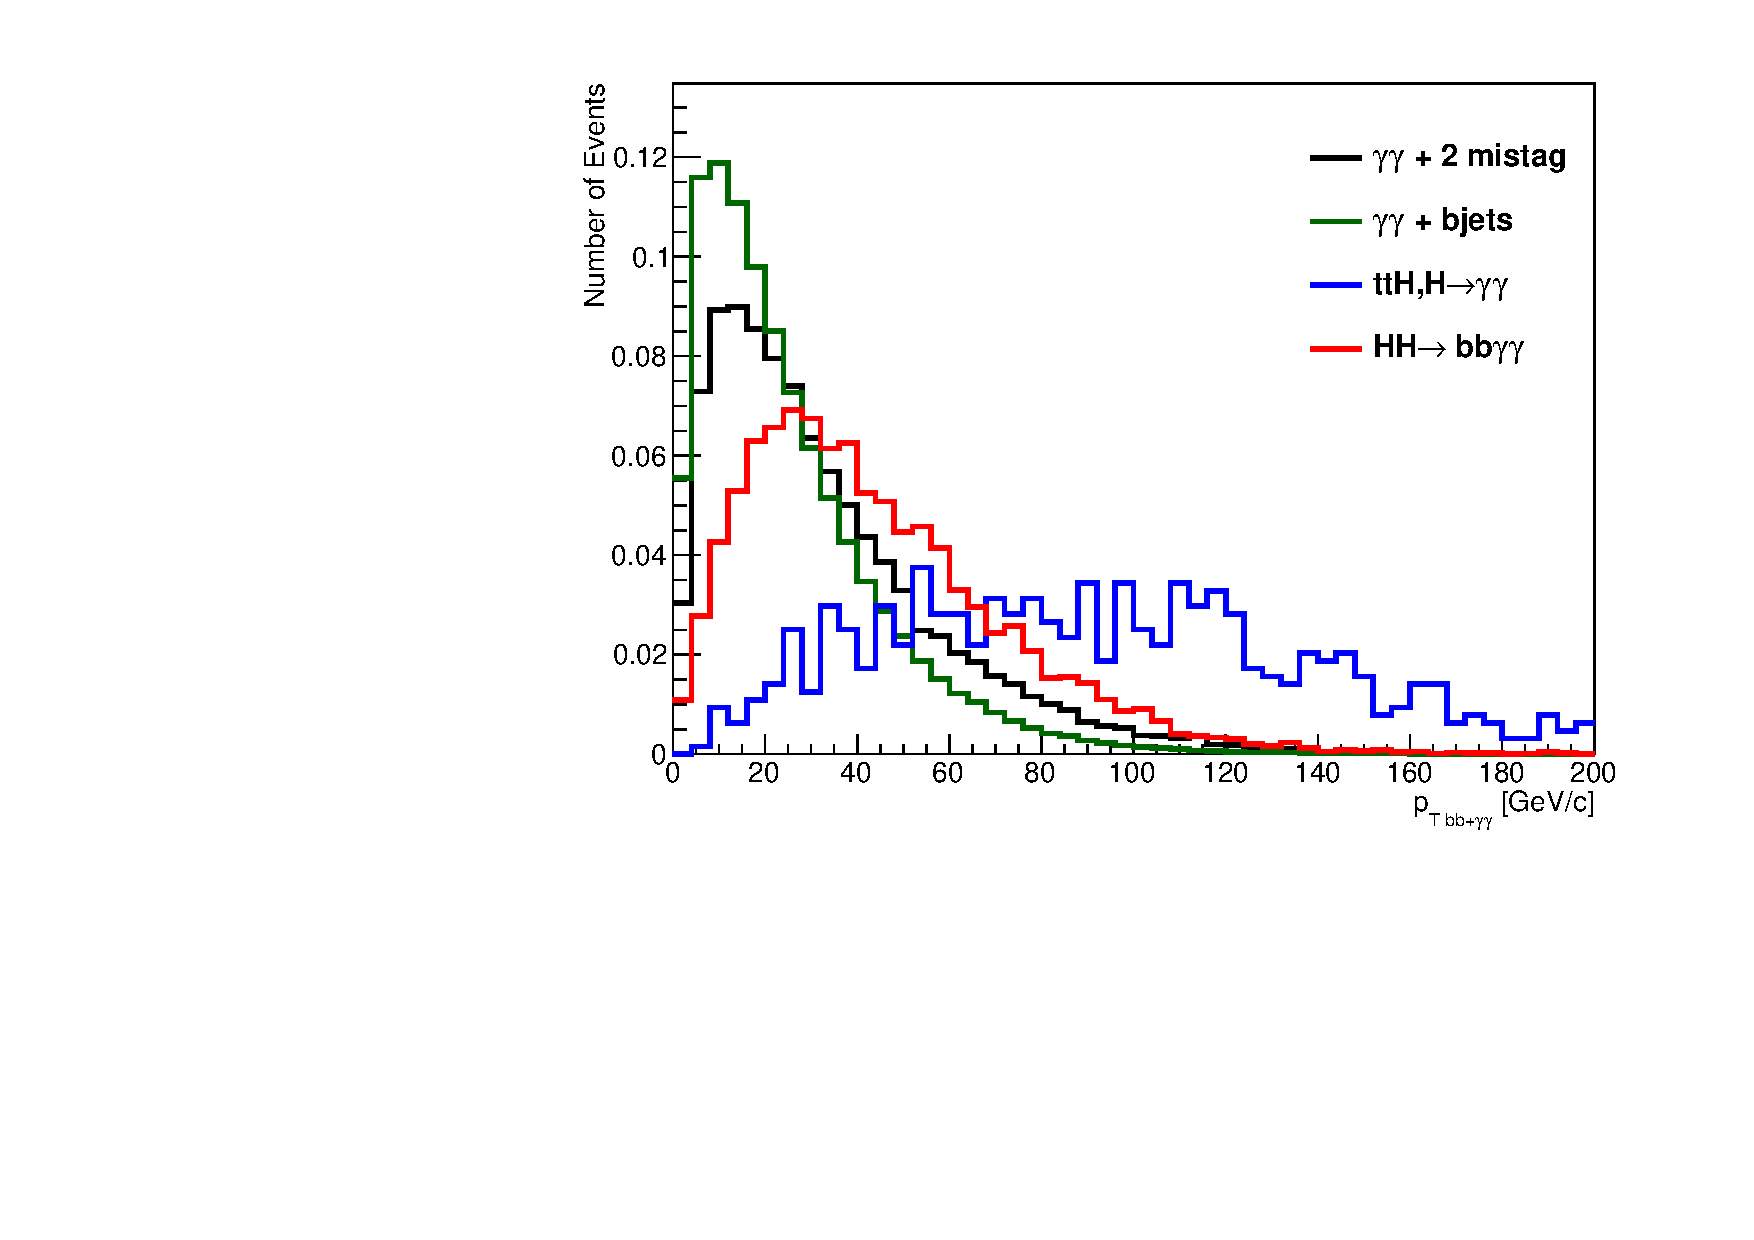
\includegraphics[scale=0.35, angle=0]{figures/Cuts/bbggPt_ps_normalized.pdf}	
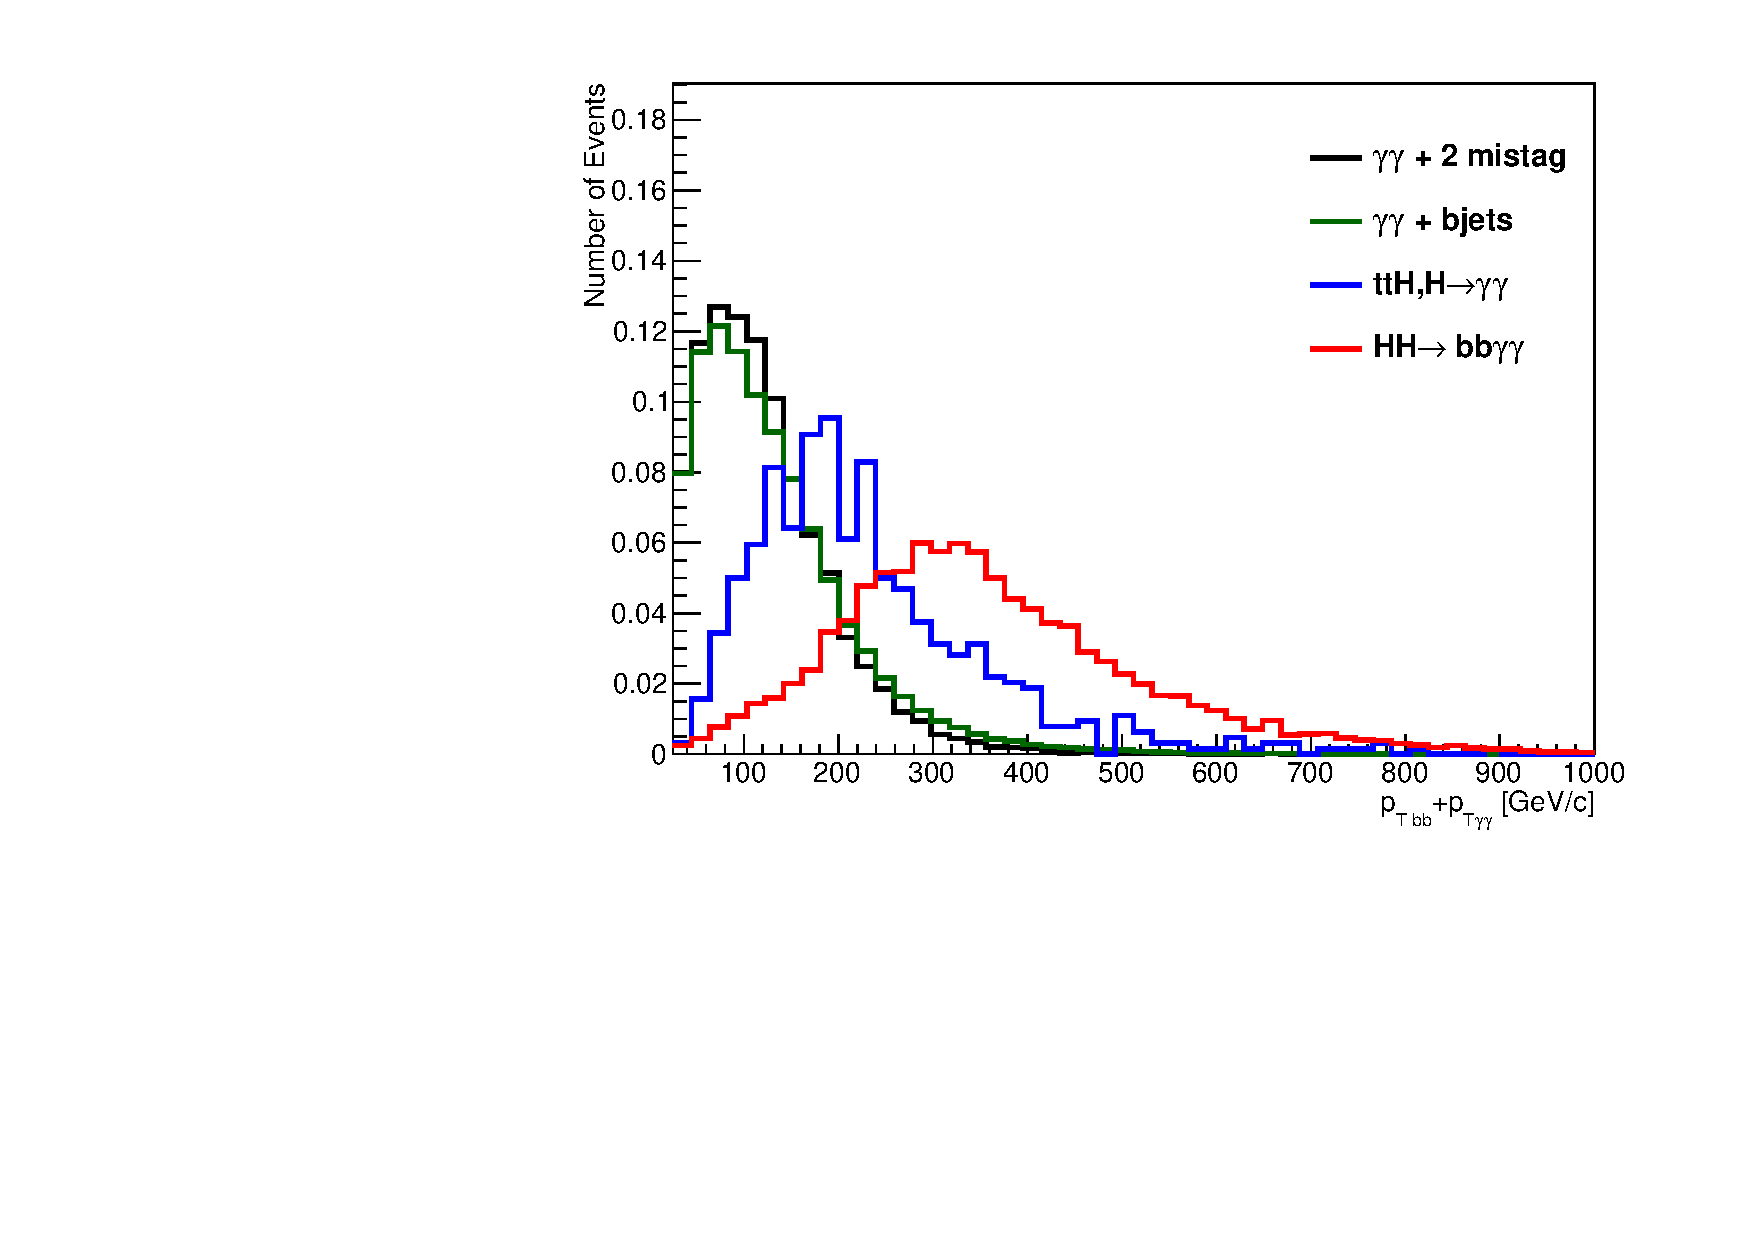
\includegraphics[scale=0.35, angle=0]{figures/Cuts/SumbbggPt_ps_normalized.pdf}	
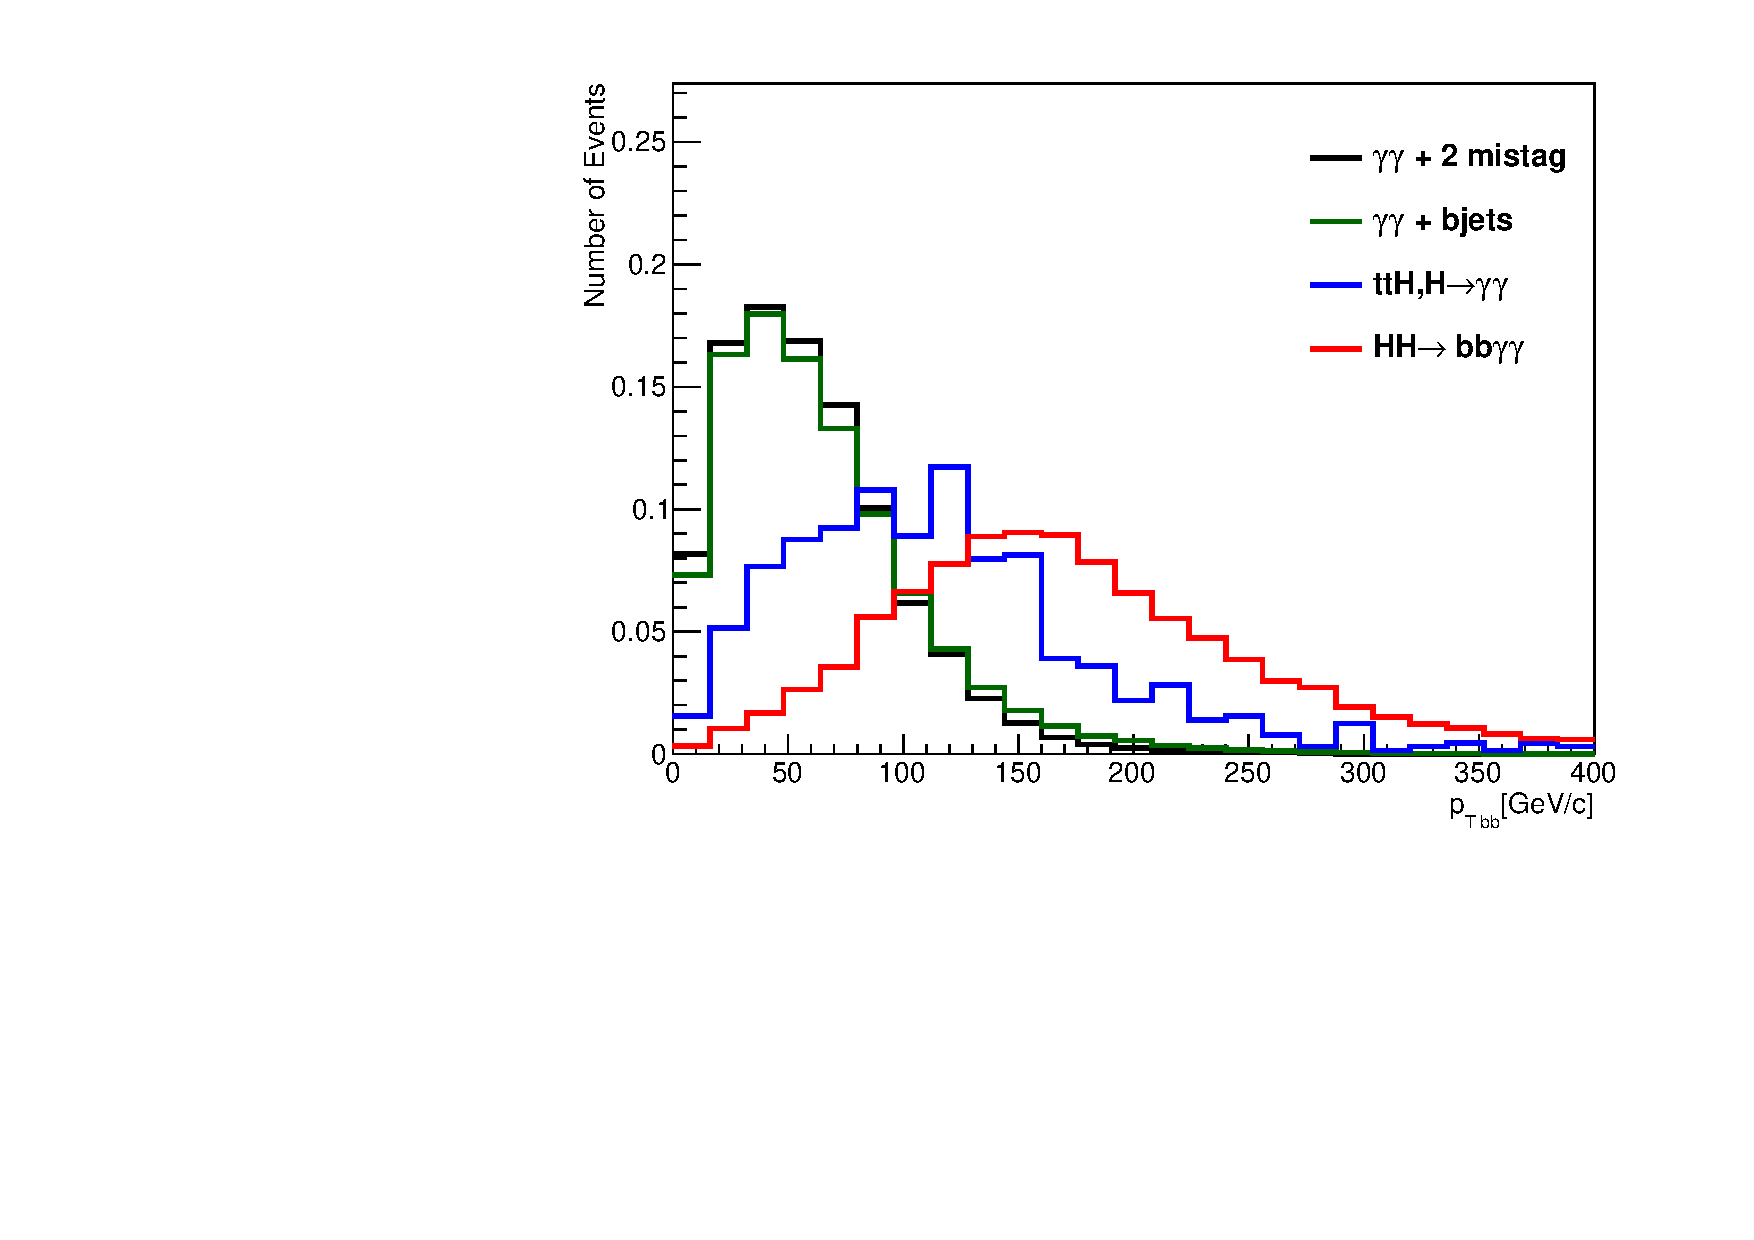
\includegraphics[scale=0.35, angle=0]{figures/Cuts/dibjetPt_ps_normalized.pdf}	
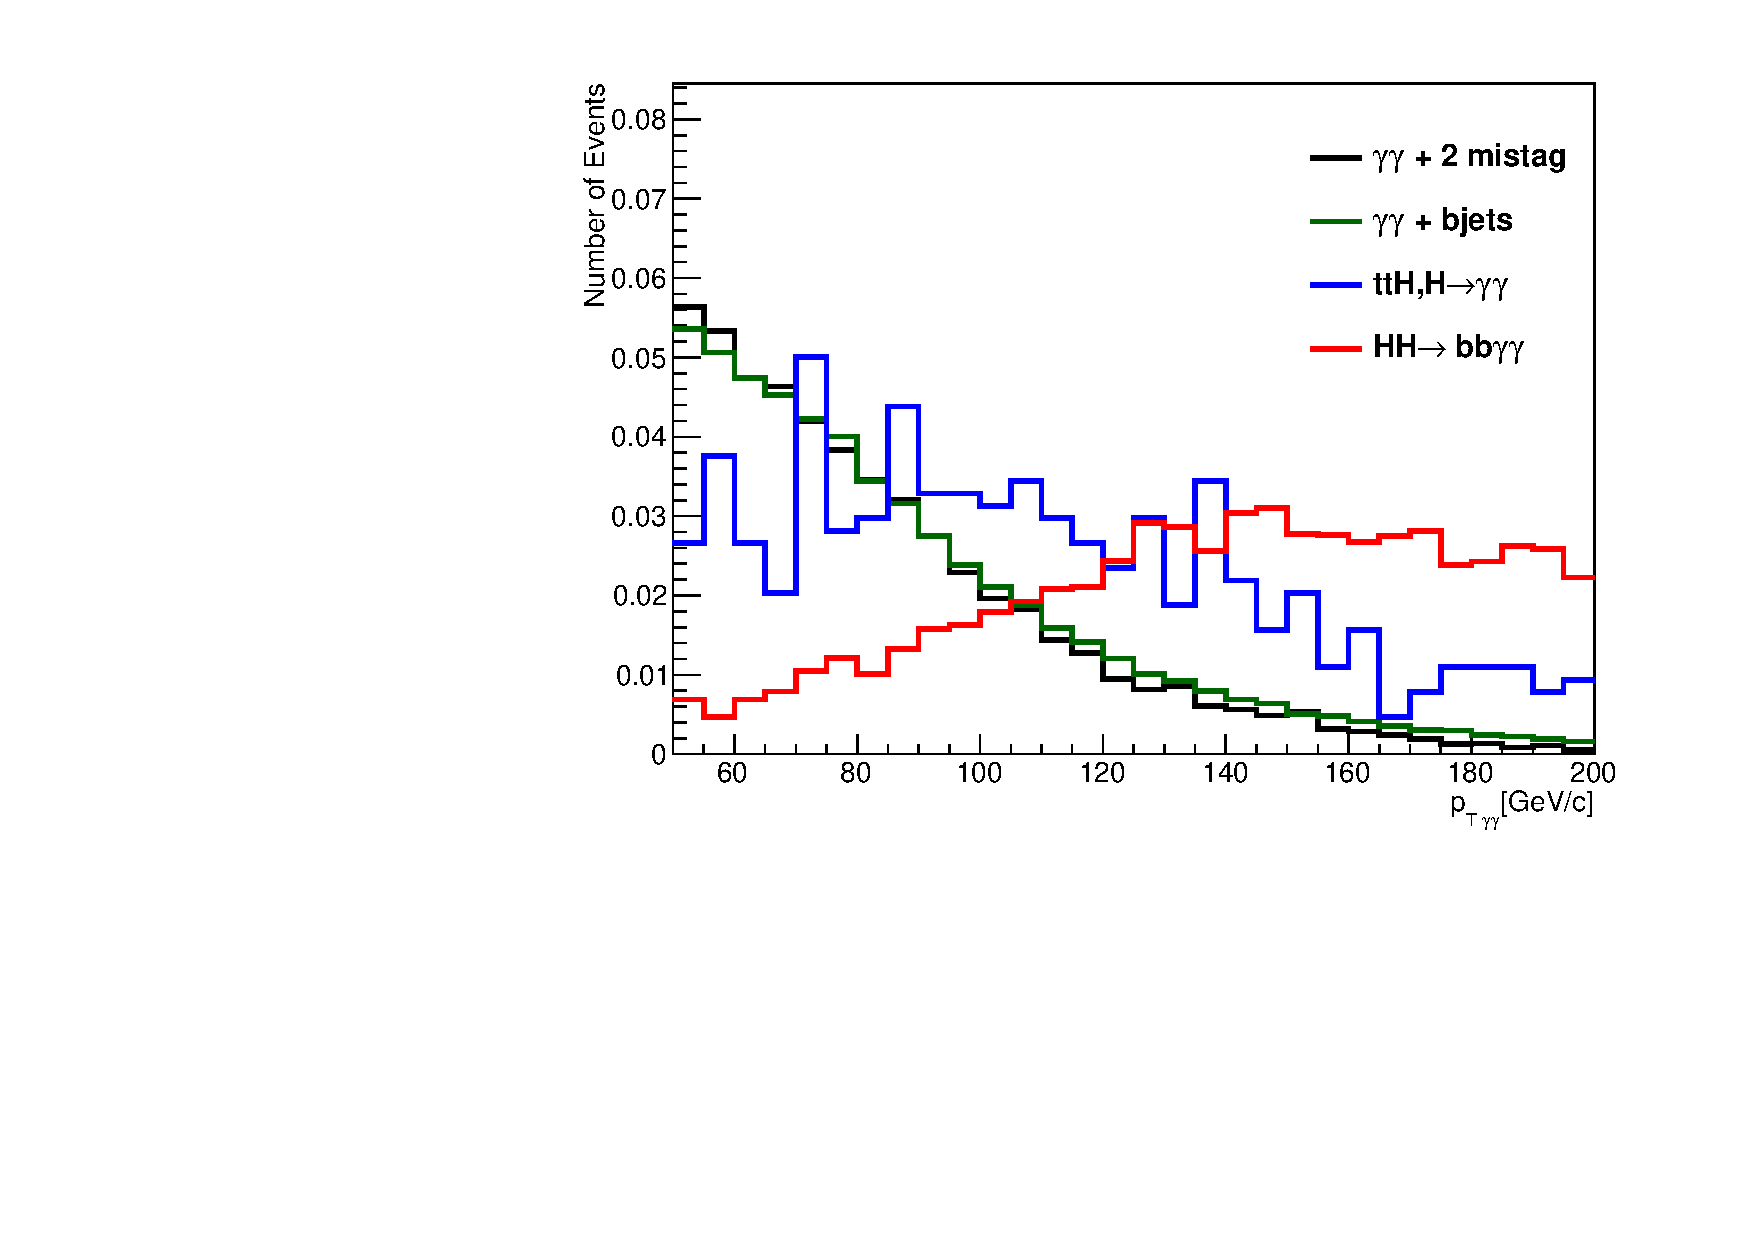
\includegraphics[scale=0.35, angle=0]{figures/Cuts/diphotonPt_ps_normalized.pdf}	
\caption{photon and b-jet $p_{T}$ distributioons post-object selection}
\label{fig:Ptcuts}
\end{figure}

\begin{table}[!ht]
\begin{center}
\begin{tabular}{|c|c|c|c|c|}   
\hline 
\multicolumn{5}{|c|}{\textbf{Expected Event Yield - $M_{bb}$: (105,145), $M_{\gamma\gamma}$: (120,130)}}\\ \hline
Sample Type                        & Scheme 0 & Scheme 1 & Scheme 2 & Scheme 1 Tight                 \\ \hline
$HH\rightarrow bb\gamma\gamma$     & 13.7     & 12.0     & 11.9     & 9.0                            \\ \hline
$ZH\rightarrow bb \gamma\gamma$    & 3.6      & 2.9      & 2.4      & 2.0                            \\ 
$ttH,H\rightarrow\gamma\gamma$     & 2.9      & 1.7      & 1.5      & 1.1                            \\ 
$bb\gamma\gamma$                   & 15.3     & 9.6      & 8.7      & 3.7                            \\ 
$jj\gamma\gamma$                   & 16.0     & 8.0      & 9.7      & 2.7                            \\ 
$jjjj$, $ccjj$, $bbjj$             & 0.2      & 0.0      & 0.0      & 0.0                            \\ 
$t\bar{t}$                         & 0.8      & 0.2      & 0.1      & 0.0                            \\ \hline
S/B Ratio                          & 0.4      & 0.5      & 0.5      & 1.0                            \\ \hline
$S/\sqrt{B}$ (Signal Significance) & 2.2      & 2.5      & 2.5      & 2.9                            \\ \hline
\end{tabular}
\caption{Expected events per cut scheme}
\label{tab:event_schemes}
\end{center}
\end{table}



We study the degree to which the different kinematic requirements alter the shape
of the diphoton and di-bjet mass distributions. In Section \ref{sec:massfits}, we describe how we 
extract the signal from the non-resonant backgrounds using maximum likelihood fits to the
diphoton and di-bjet mass distributions. For this analysis method, it is critical that any of the kinematic selection cuts
that we apply preserves the smooth and monotonic behavior of the non-resonant background. Any
peak-like feature that is introduced in the non-resonant background as a result of any of the
kinematic selection cuts would bias the determination of the background from the fit and would lead
to a bias of the cross section measurement. 

In Figure \ref{fig:Mbb_Mgg}, we show the distributions of the diphoton and di-bjet mass after the 
``Scheme0'', ``Scheme1'', and ``Scheme2'' selection requirements for the non-resonant 
$b\bar{b}\gamma\gamma$ background. We note that the ``Scheme 0'' and the ``Scheme 1'' selection 
cuts do preserve the general exponentially decaying trend in the mass distributions, 
however the ``Scheme 2''  selection cuts appear to significantly change the shape of the 
mass distributions. They still appear smooth and monotonic, but are significantly more flat,
and with a more severe inflection in the case of the diphoton mass. Therefore, we prefer
the ``Scheme 1'' cuts and all following discussion will use the ``Scheme 1'' selection
by default. 

\begin{figure}[h]
\centering
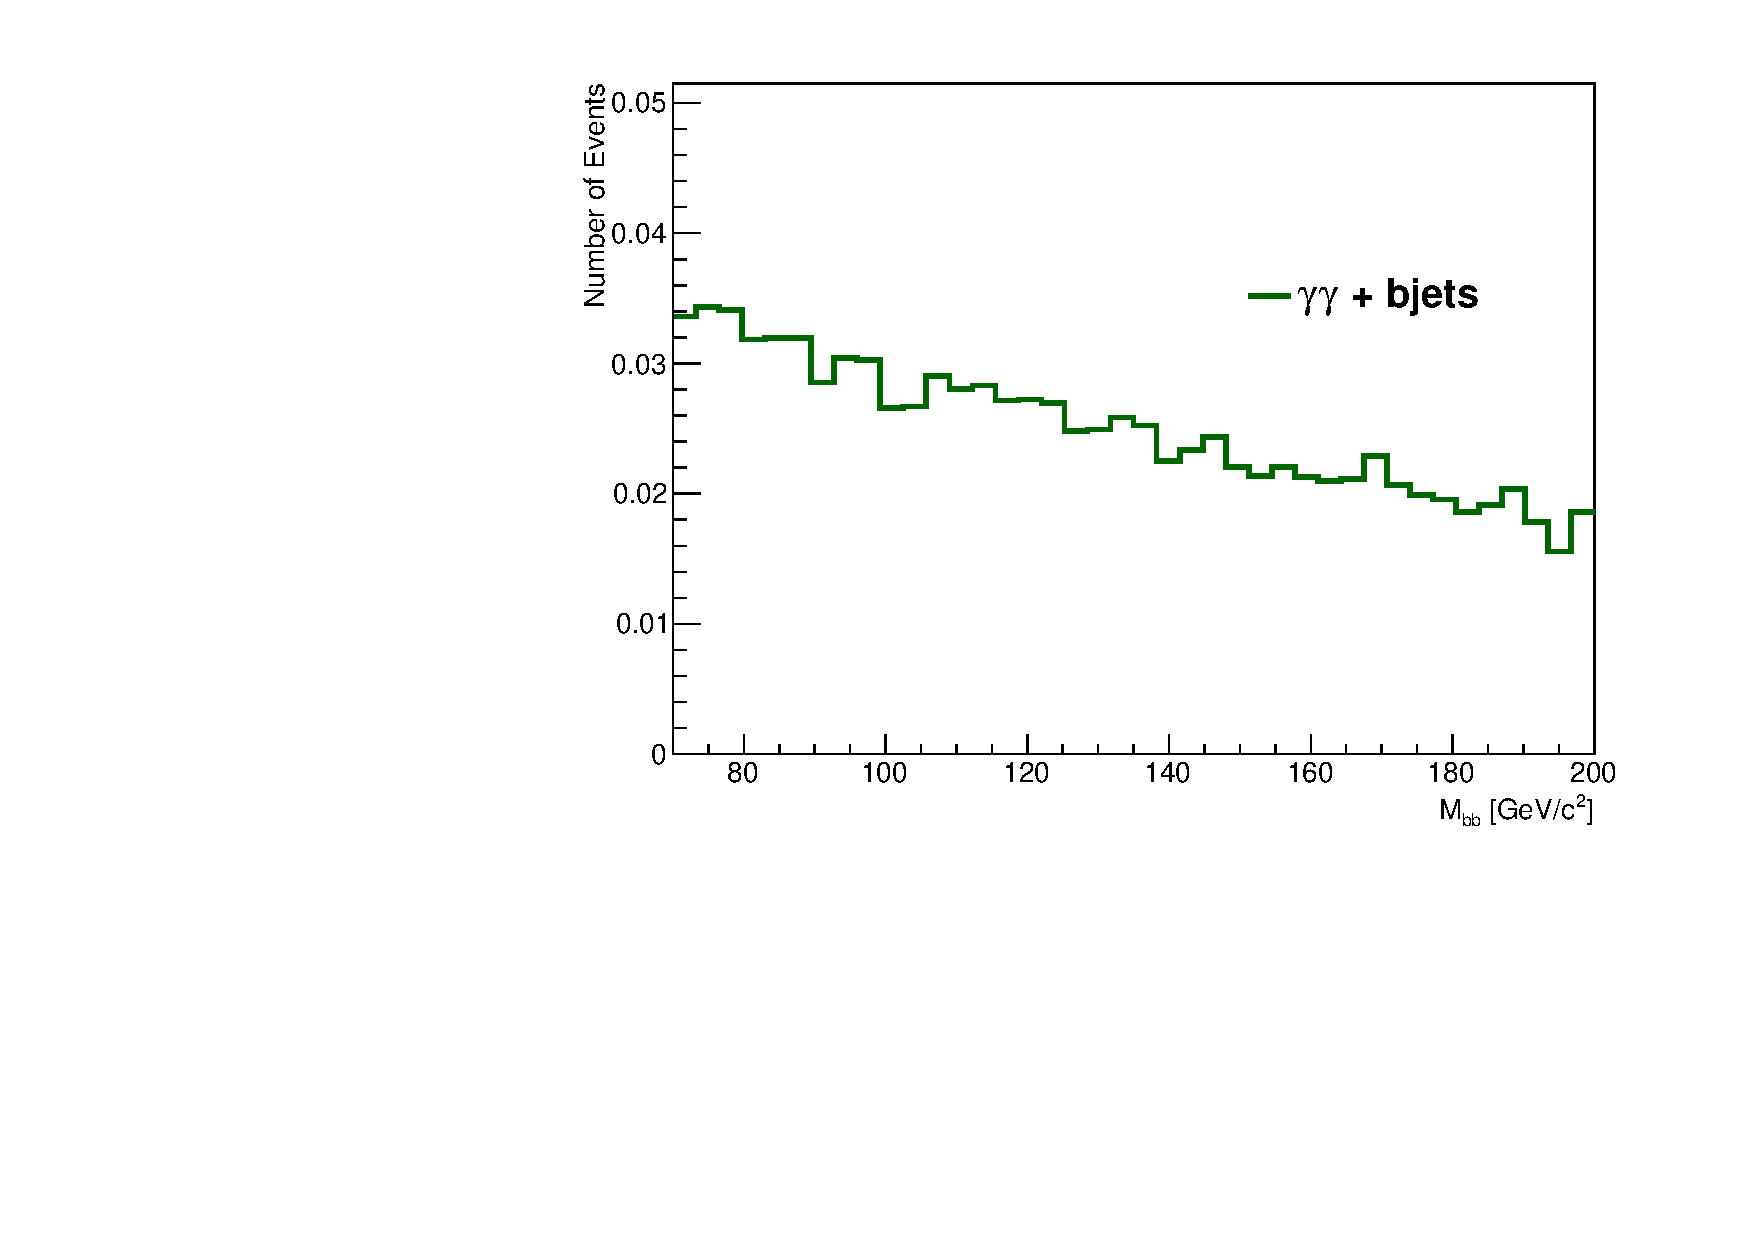
\includegraphics[scale=0.35, angle=0]{figures/Cuts/MassBB_s0.pdf}	
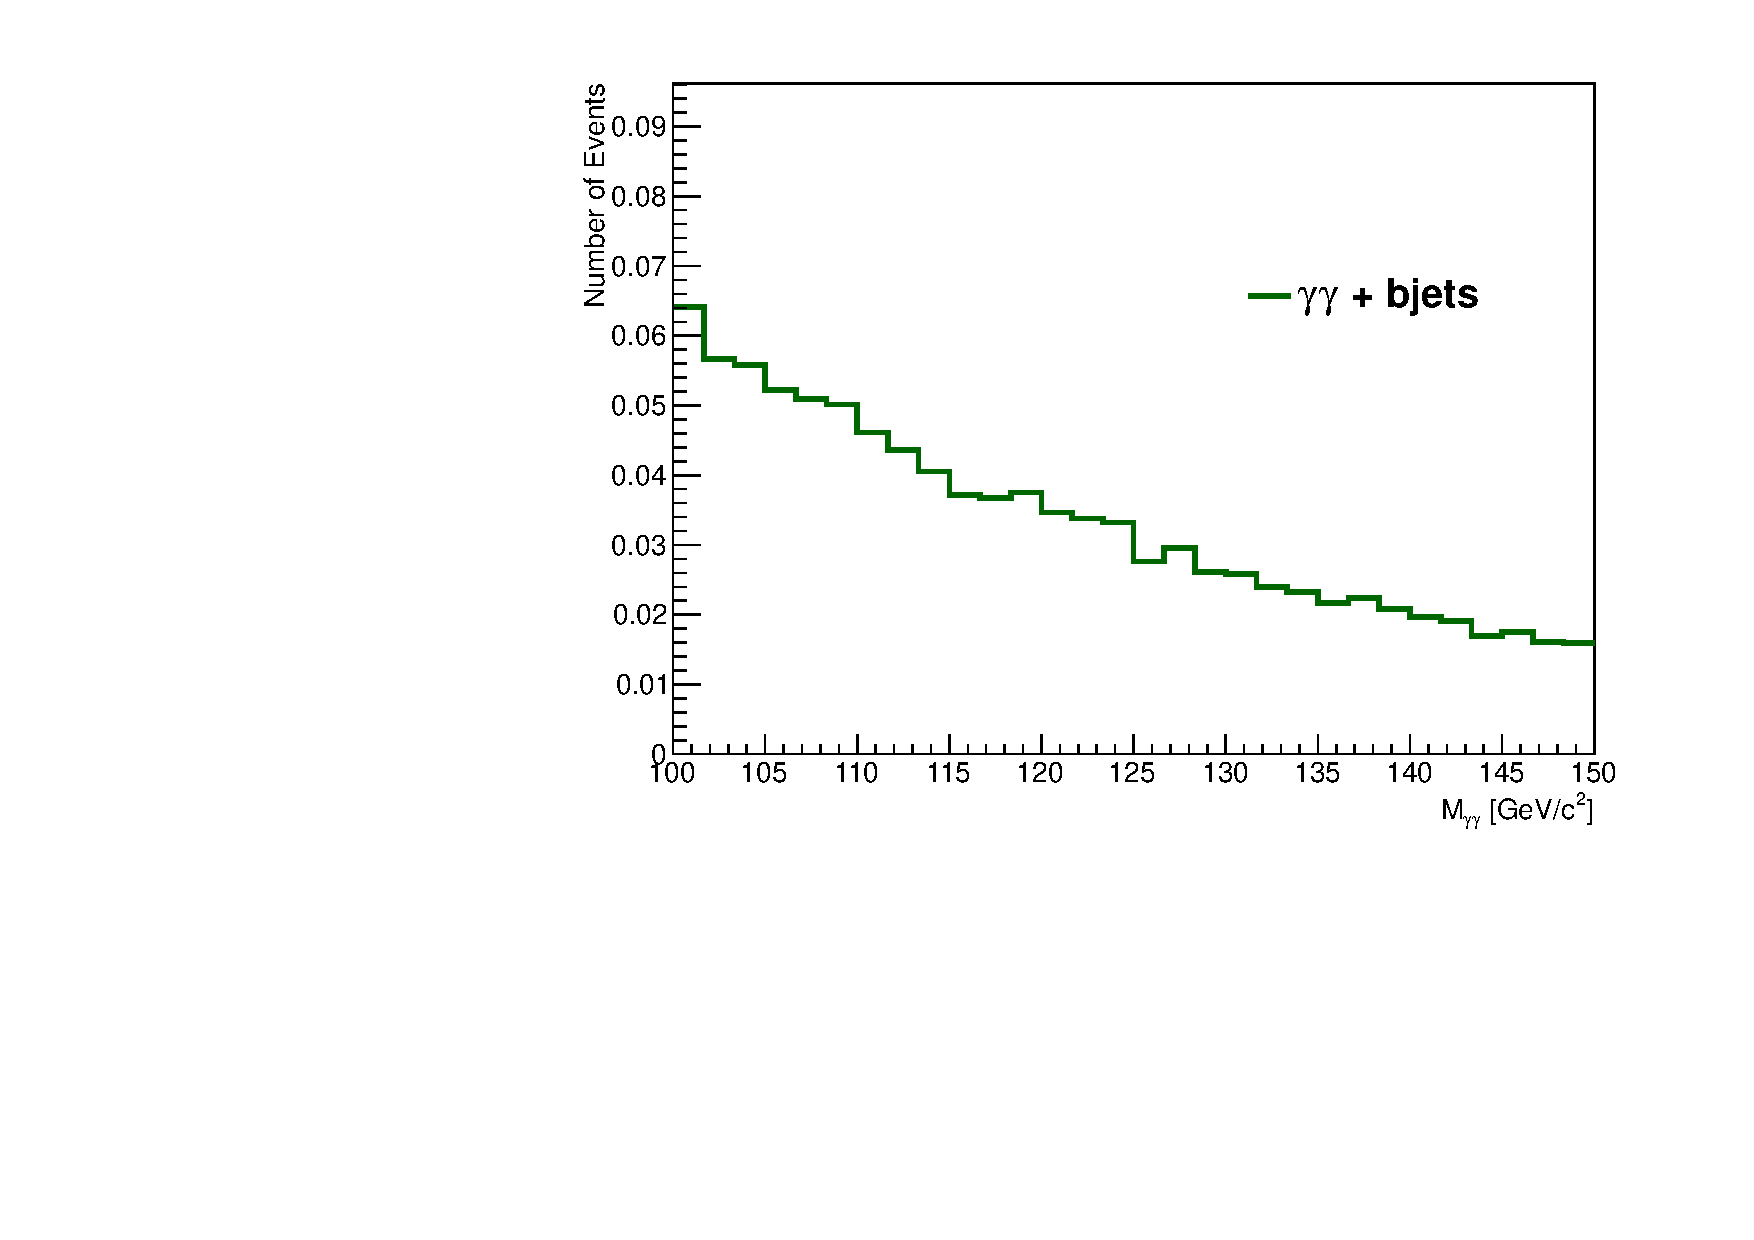
\includegraphics[scale=0.35, angle=0]{figures/Cuts/MassGG_s0.pdf}	
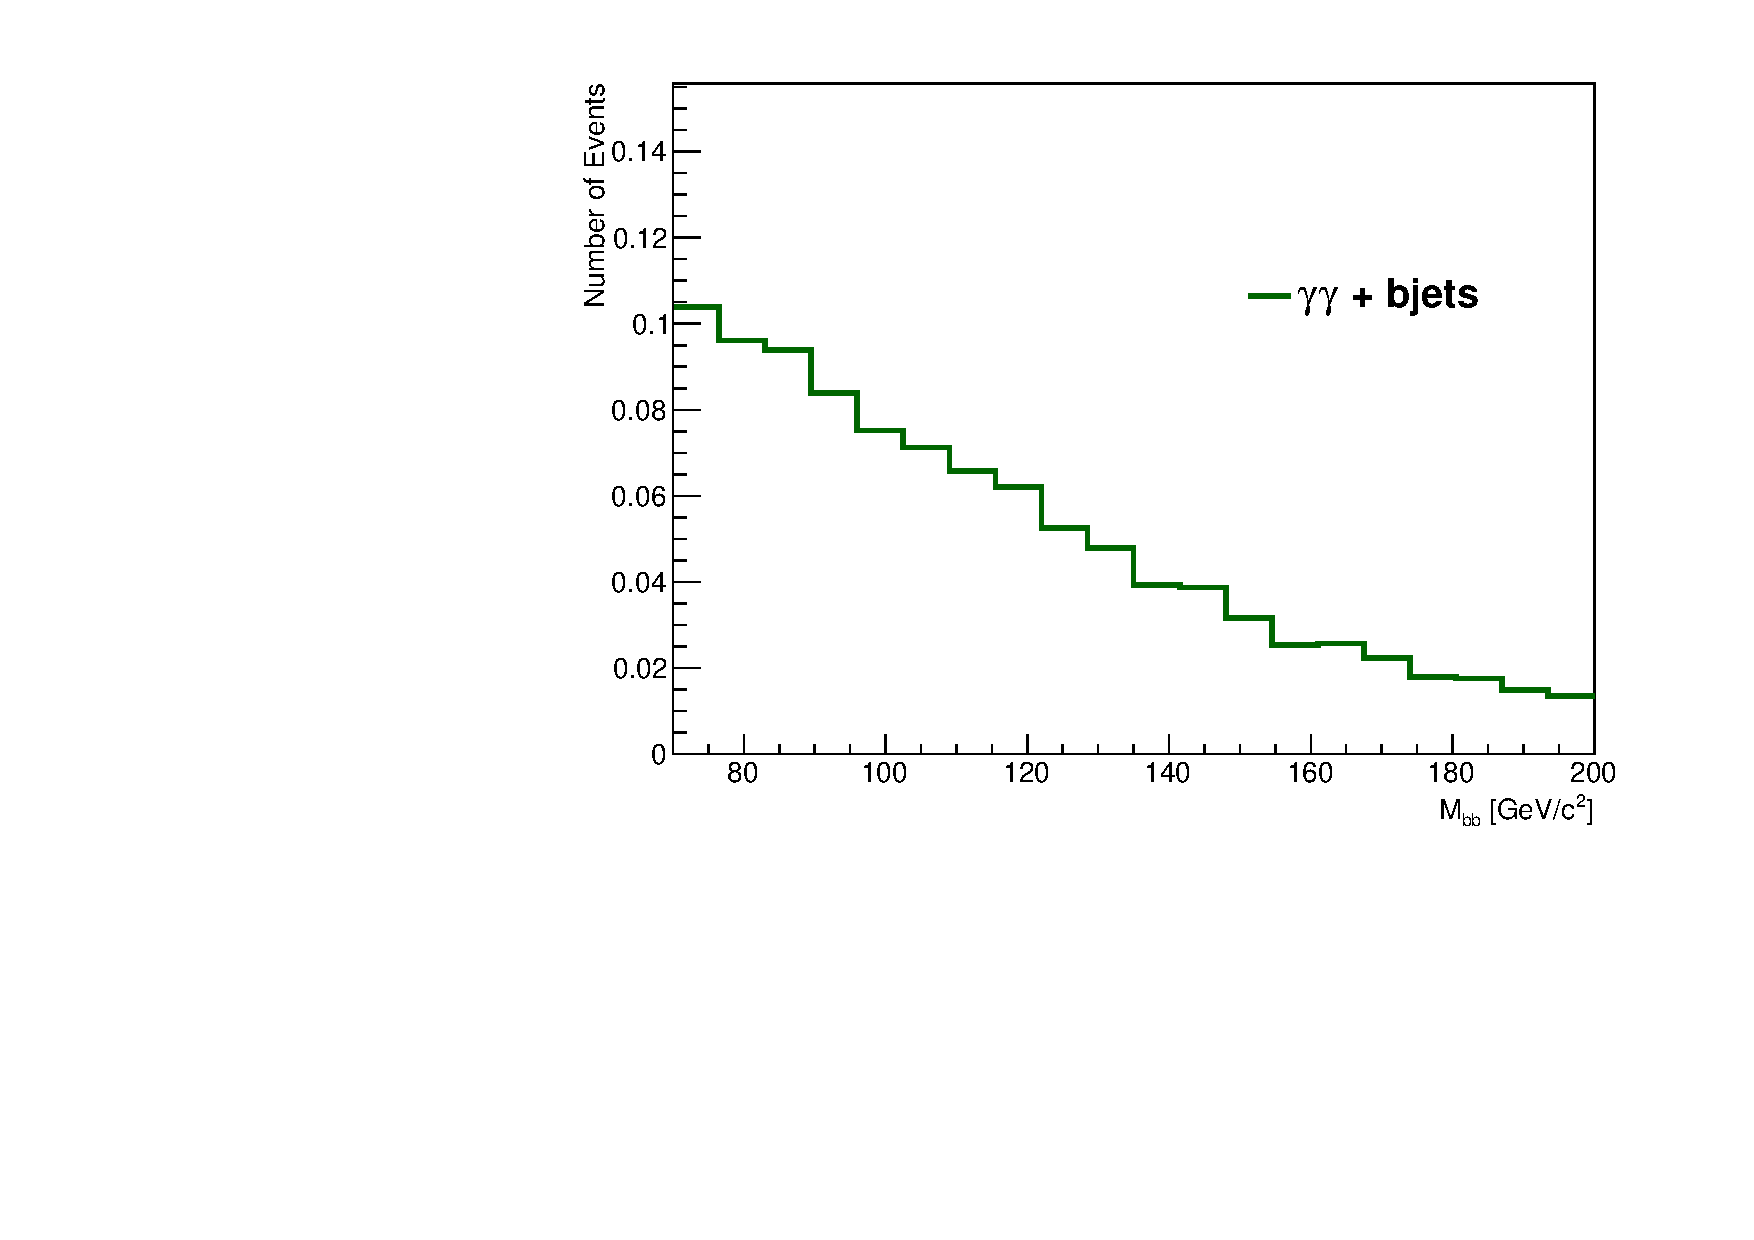
\includegraphics[scale=0.35, angle=0]{figures/Cuts/MassBB_s1.pdf}	
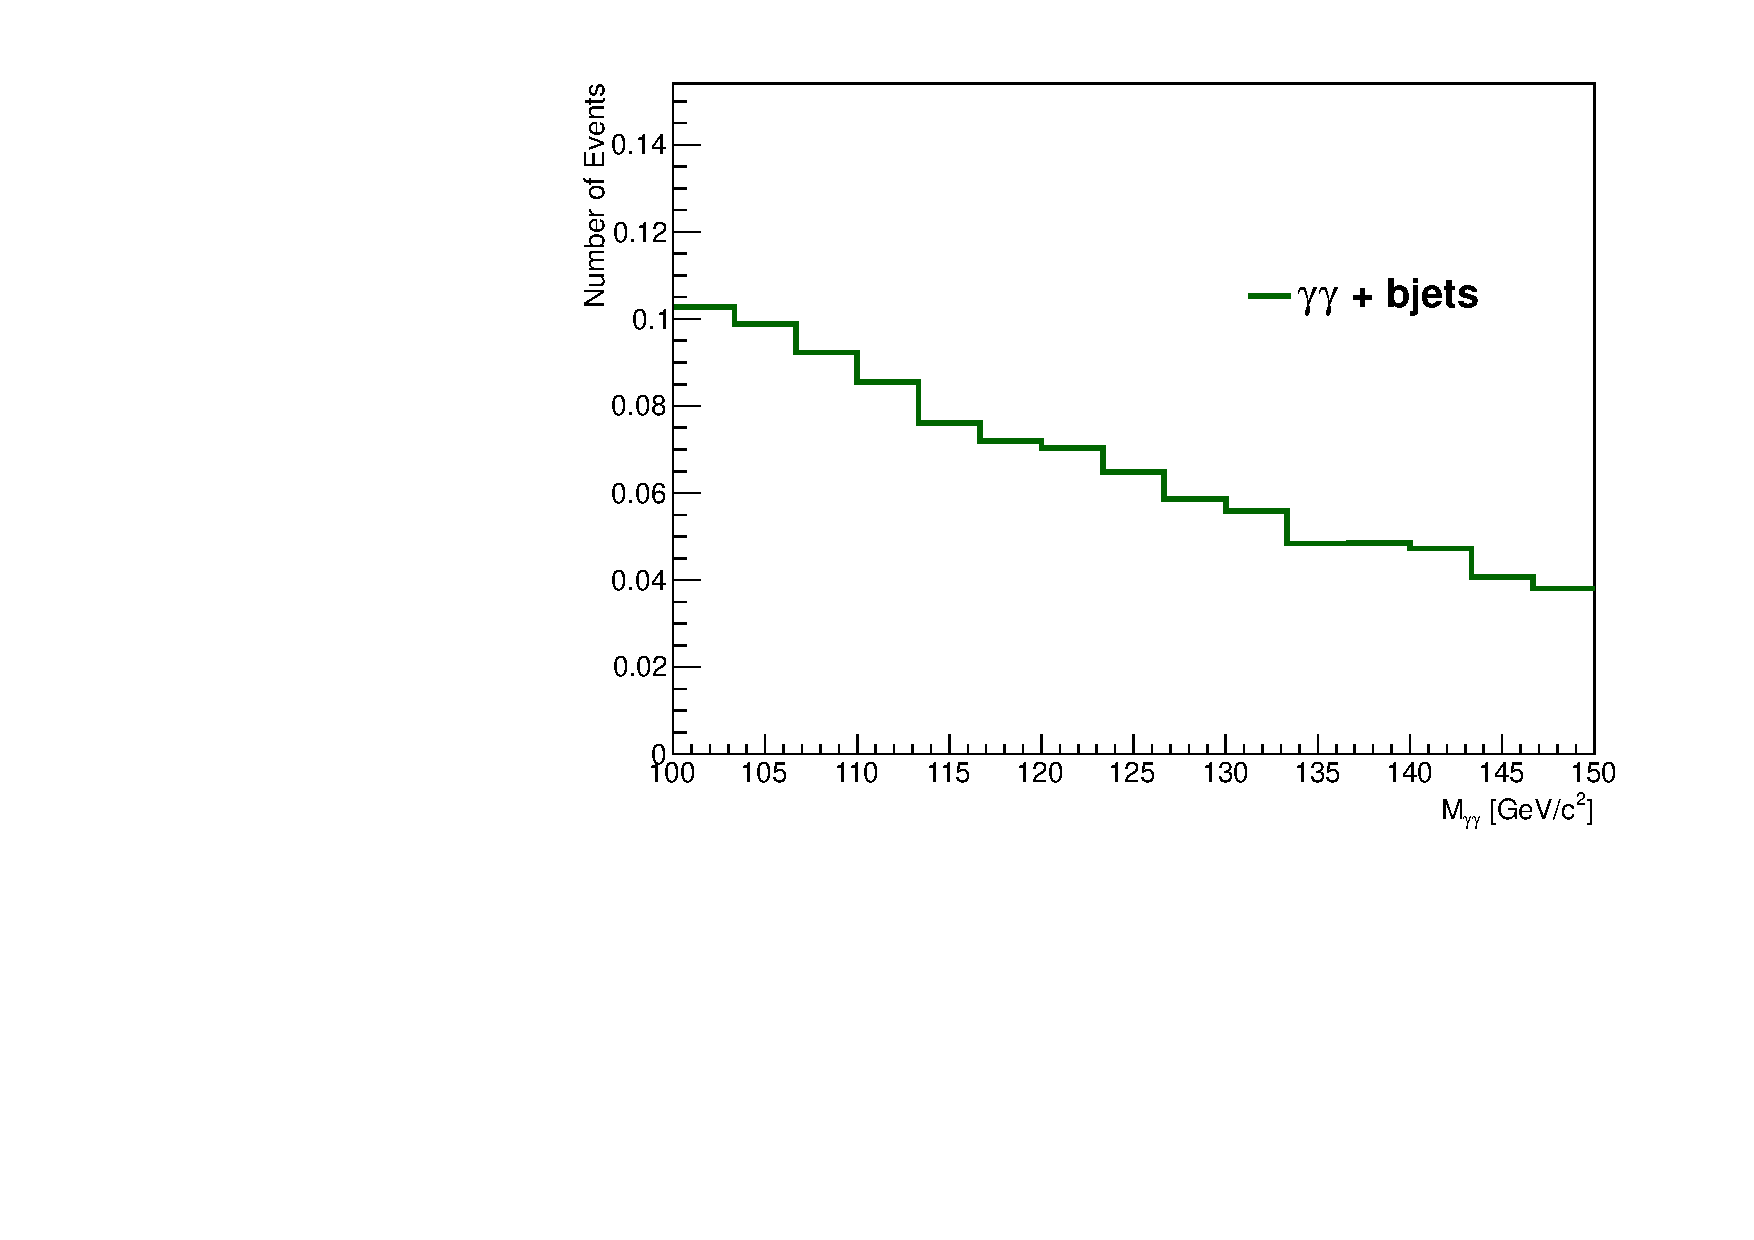
\includegraphics[scale=0.35, angle=0]{figures/Cuts/MassGG_s1.pdf}	
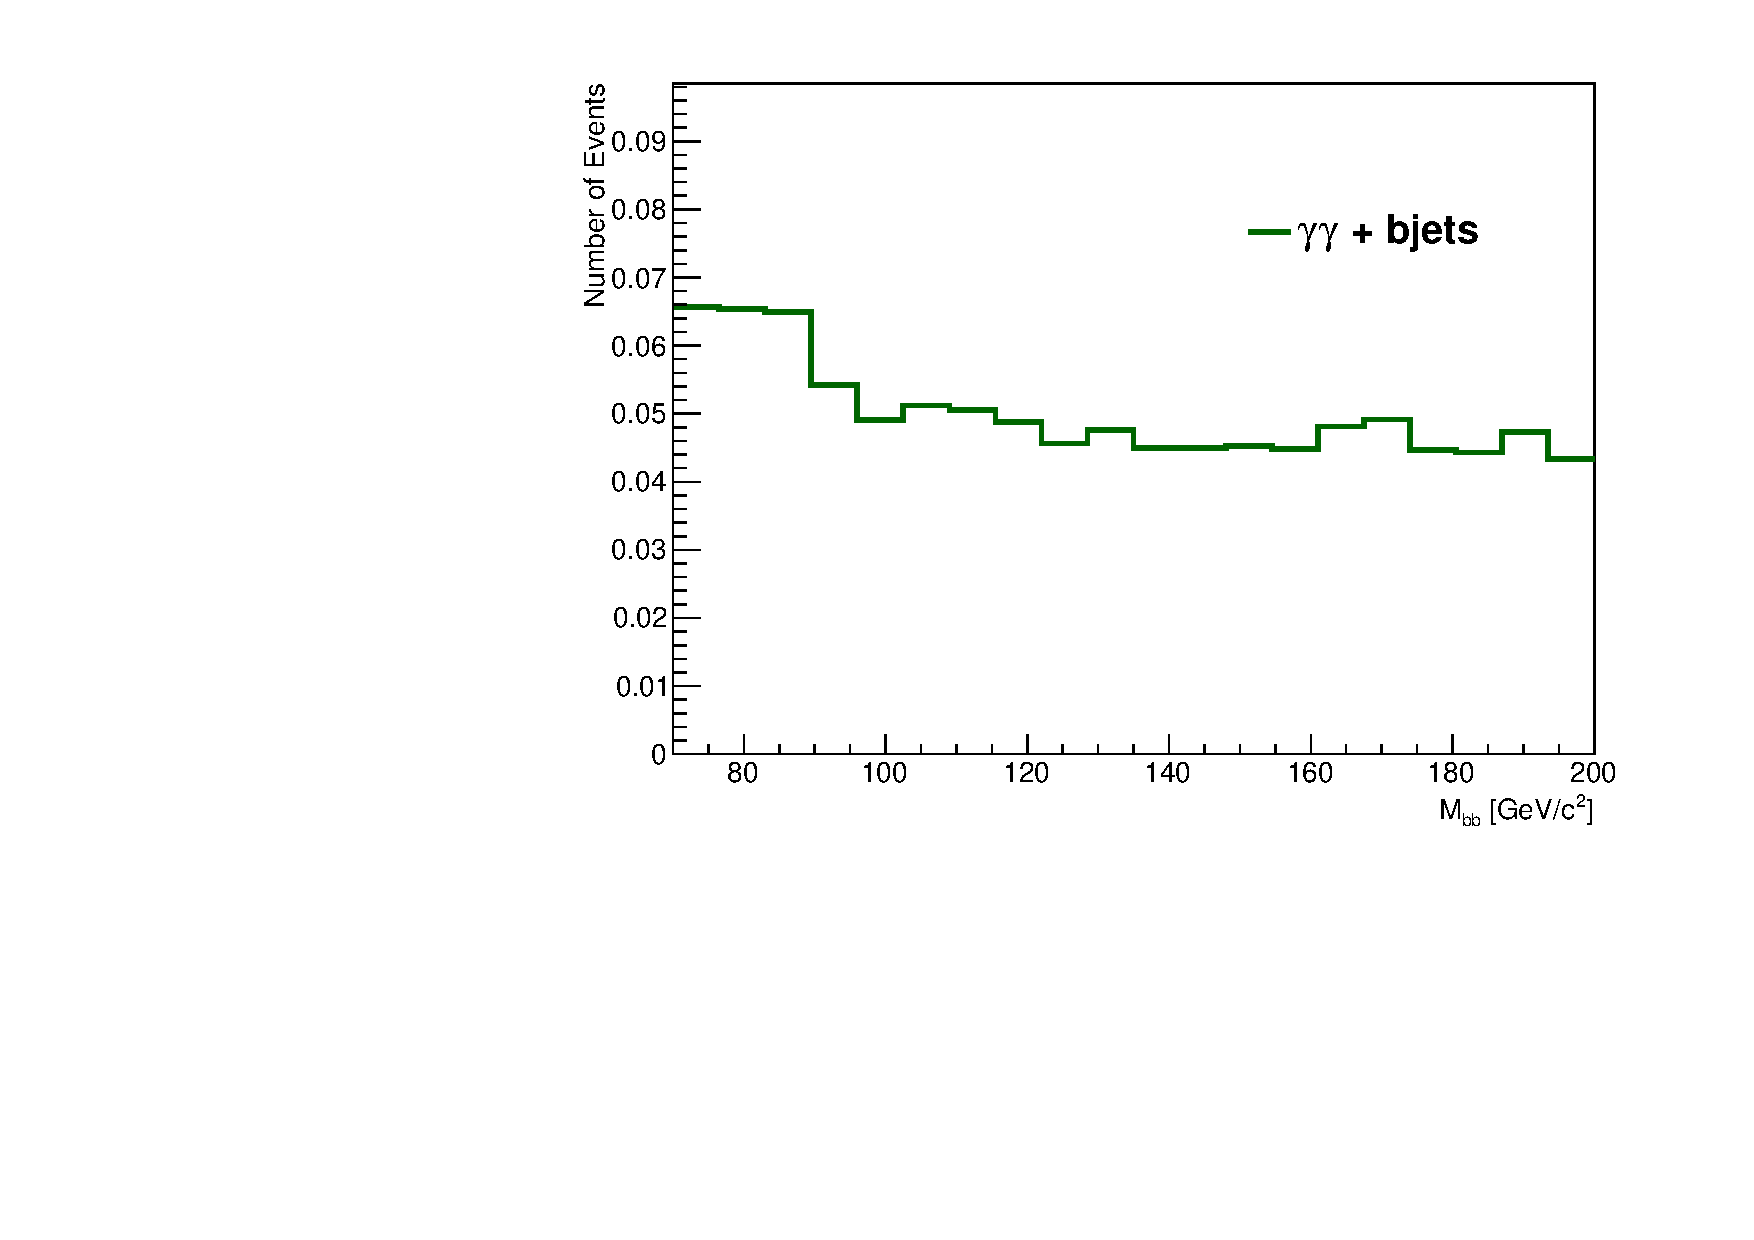
\includegraphics[scale=0.35, angle=0]{figures/Cuts/MassBB_s2.pdf}	
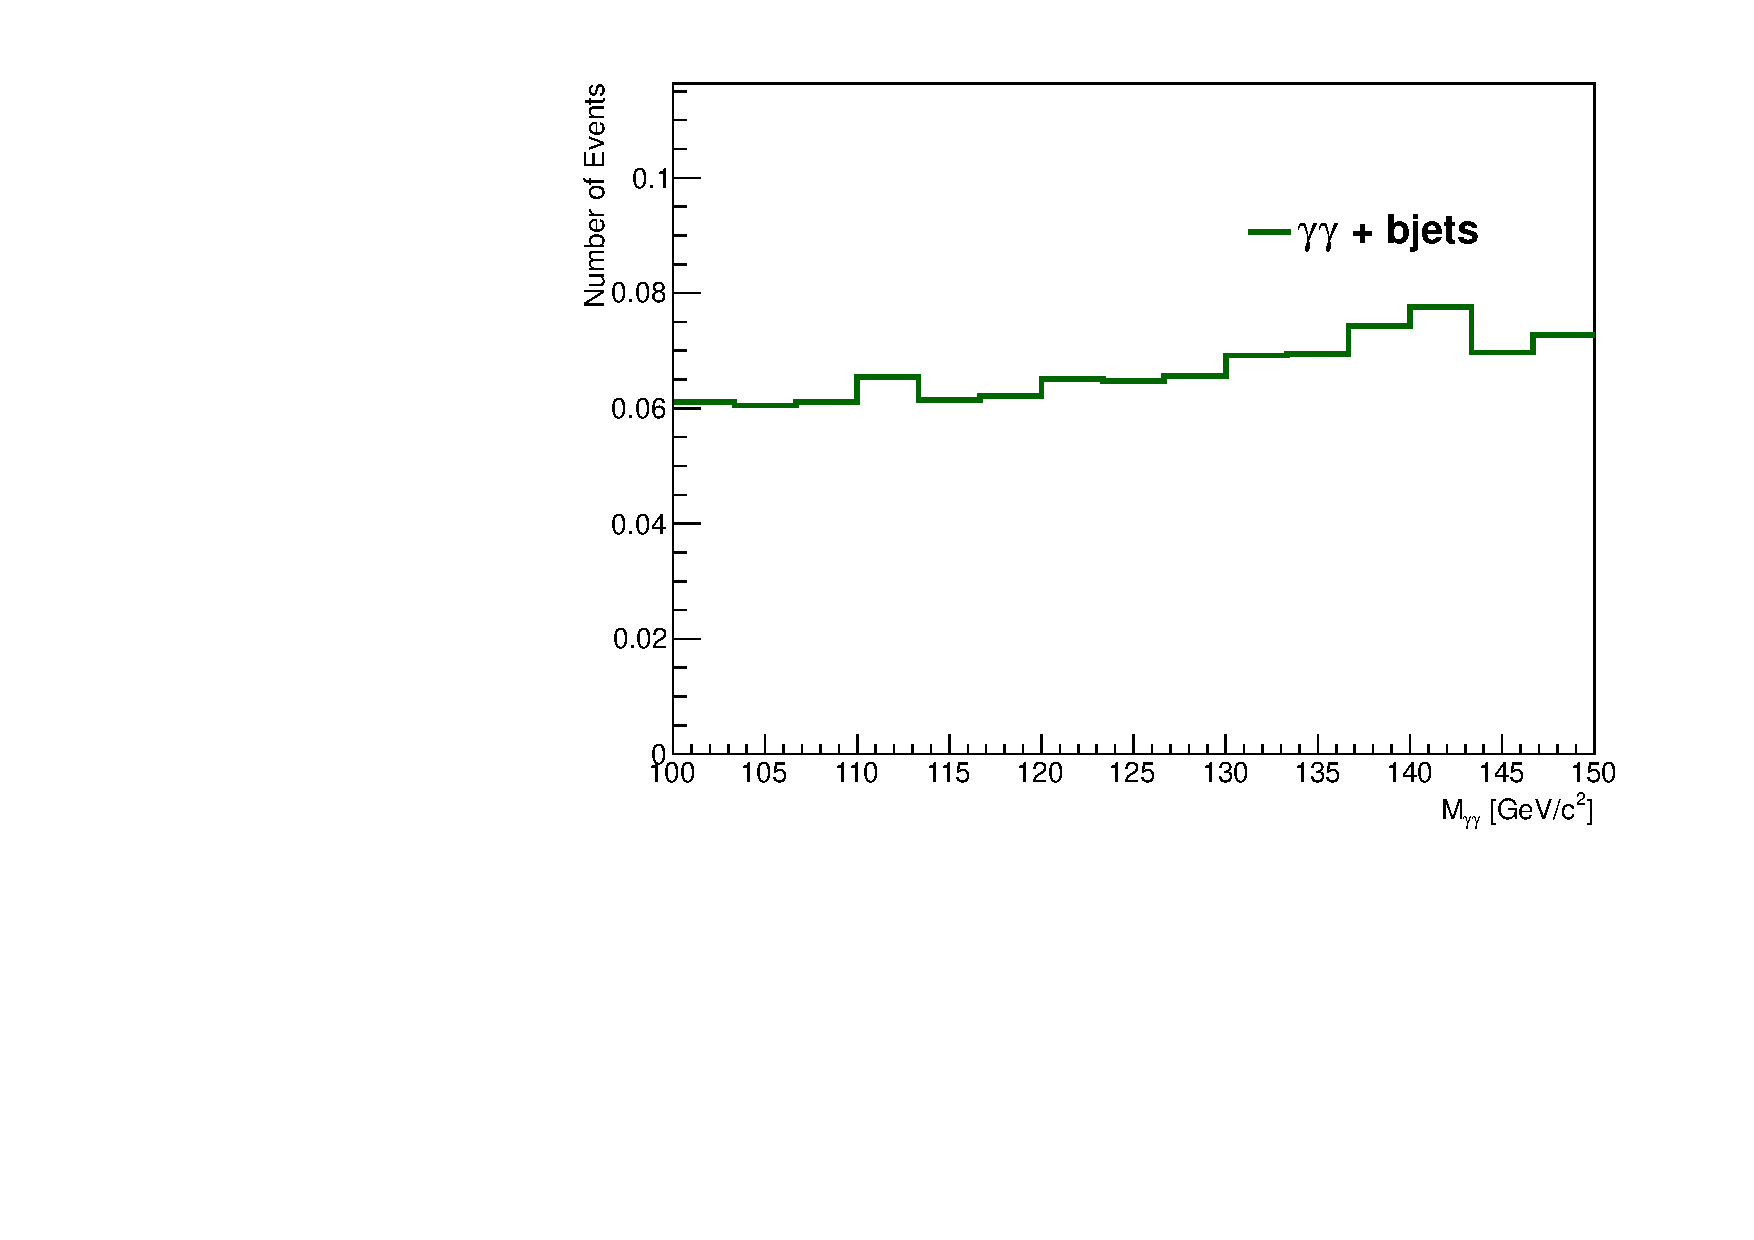
\includegraphics[scale=0.35, angle=0]{figures/Cuts/MassGG_s2.pdf}	
\caption{diphoton and di-bjet mass backgrounds}
\label{fig:Mbb_Mgg}
\end{figure}



\section{Signal and Background Estimation}
\label{sec:bkgestimation}
The signal process of interest is the production of two Higgs bosons, one of which decays to a pair of b quarks, 
and the other decaying to a pair of photons. 
The backgrounds can be broadly categorized into resonant backgrounds which contain one Higgs boson 
decaying to two photons, and non-resonant backgrounds which do not contain a Higgs boson. 
Where available, we use full simulation Monte Carlo samples of the current Run1 CMS detector.
For the remaining backgrounds we generate samples using madgraph, perform the parton showering and
hadronization using Pythia, and then apply weights to account for the object selection efficiencies
and fake rates.

\subsection{$HH \rightarrow bb\gamma\gamma$ Signal}
The signal process is generated with Madgraph using a custom model for the Di-Higgs process. The parton
shower and hadronization effects are modelled using Pythia, and a GEANT-based full detector simulation 
of the current Run1 CMS detector is performed. Next, we apply the object selection requirements as 
described above in Section \ref{sec:objects}, and apply the event selection requirements as described 
in Section \ref{sec:eventselection}. The Monte Carlo sample is normalized to a signal cross section
times branching ratio of $0.089$~fb. In Table \ref{tab:signalEventYields}, we show the 
expected event yields for $3 ab^{-1}$ of integrated luminosity at various stages of the event
selection.


\begin{table}[!ht]
\begin{center} 
\begin{tabular}{|c|c|c|}
\hline
Selection Stage       &  Signal Event Yield &  \\  \hline
Object Selection                &  00000       \\ 
Kinematic Selection ($\Delta$R) &  00000       \\ 
Mass Windows                    &  00000       \\ \hline

\end{tabular}
\caption{Expected Signal Yields }
\label{tab:signalEventYields}
\end{center}
\end{table}

\subsection{Resonant Backgrounds}
The main backgrounds involving a Higgs boson are $ZH$, where a Higgs boson is produced in association
with a Z boson which subsequently decays to two b-jets, $t\bar{t}H$, where a Higgs boson is produced
in associated with a top and anti-top quark pair, and $b\bar{t}H$, where a Higgs boson is produced in
association with a b and anti-b quark pair. Table \ref{} shows the cross sections for these processes
for a center of mass energy of $14$~TeV.


\begin{table}[!ht]
\begin{center} 
\begin{tabular}{|c|c|}
\hline
Process                                           &   Cross Section $\times$ BR (fb)   \\  \hline
$ZH \rightarrow b\bar{b}\gamma\gamma$             &   $2.01$                           \\\hline
$t\bar{t}H \rightarrow W W b \bar{b}\gamma\gamma$ &   $1.39$                           \\\hline

\end{tabular}
\caption{Resonant Bkg Cross Sections }
\label{tab:ResonantBkgCrossSections}
\end{center}
\end{table}

The $ZH$ and $t\bar{t}H$ backgrounds are estimated using full simulation samples. For reasons of 
availability, these full simulation samples are produced for a center of mass energy of $8$~TeV.
The event yields for these background processes expected for $3 ab^{-1}$ of integrated luminosity
are shown in Table \ref{tab:resonantBkgEventYields} at various stages of the event selection.

\begin{table}[!ht]
\begin{center} 
\begin{tabular}{|c|c|c|}
\hline
Process / Selection Stage       &  $ZH \rightarrow b\bar{b}\gamma\gamma$ &  $t\bar{t}H \rightarrow W W b \bar{b}\gamma\gamma$    \\  \hline
Object Selection                &  00000                                 &  00000                                                \\ 
Kinematic Selection ($\Delta$R) &  00000                                 &  00000                                                \\ 
Mass Windows                    &  00000                                 &  00000                                                \\ \hline

\end{tabular}
\caption{Expected Resonant Background Yields }
\label{tab:resonantBkgEventYields}
\end{center}
\end{table}


%some words about bbH...%
%some words about systematic error of using 8TeV samples?%



\subsection{Non-resonant Backgrounds}
The non-resonant backgrounds include QCD production of $b \bar{b} \gamma\gamma$, QCD production
of $jj \gamma\gamma$ with light jets mistagged as b-jets, QCD production of $b \bar{b} jj$ with
jets mis-identified as photons, and QCD production of four jets with two jets mis-identified 
as photons and two jets mistagged as b-jets. These background processes have cross sections
that are several orders of magnitude larger than the resonant backgrounds, but are suppressed
by the low rate for mistags and mis-identified photons. Due to their large cross sections, 
it is computationally impossible to fully simulate these background events. Instead, we adopt the
approach of producing generator particle level Monte Carlo samples and weight the events by the
corresponding efficiencies for selecting the constituent particles.

All QCD background processes are generated using Madgraph \cite{madgraph} with particular kinematic
cuts in order to focus in on the phase space of interest. Table \ref{tab:MadgraphBkgCrossSections} 
summarizes the different QCD processes that were produced, their cross sections, 
and any phase space requirements that were applied. Pythia is used to perform parton showering,
and hadronization, and particle level jet clustering is performed. The efficiencies, fake rates, and
mistag rates are applied as a function of the jet $\eta$ and $p_{T}$ according to the measurements
from the full simulation samples shown in Figures \ref{fig:photonEfficiency} to \ref{fig:mistagRate}.


\begin{table}[!ht]
\begin{center} 
\begin{tabular}{|c|c|c|}
\hline
Process                  &   Cross Section (fb)   &  Phase Space Cuts                                         \\  \hline
$b \bar{b} \gamma\gamma$ &   $136.4$              &  $p_{T b} > 20$~GeV, $p_{T \gamma} > 20$~GeV, $|\eta_{\gamma}| < 3.0$, $|\eta_{b}| < 3.0$   \\
                         &                        &  $ 60 < M_{\gamma\gamma} < 200$, $ 60 < M_{bb} < 200$     \\\hline
$jj \gamma\gamma$        &   $22440$              &  $p_{T j} > 20$~GeV, $p_{T \gamma} > 20$~GeV, $|\eta_{\gamma}| < 3.0$    \\
                         &                        &  $ 60 < M_{\gamma\gamma} < 200$, $ 60 < M_{jj} < 200$     \\\hline
$bb jj$                  &   $2.14 \times 10^{8}$ &  $p_{T b} > 20$~GeV, $p_{T j} > 20$~GeV, $|\eta_{b}| < 2.5$, $|\eta_{j}| < 2.5$      \\
                         &                        &  $ 90 < M_{bb} < 160$  , $110 < M_{jj} < 140$,            \\\hline
$cc jj$                  &   $2.14 \times 10^{8}$ &  $p_{T j} > 20$~GeV, $|\eta_{j}| < 2.5$                   \\
                         &                        &  $110 < M_{jj} < 140$,                                    \\\hline
$jjjj$                   &  $2.04 \times 10^{10}$ &  $p_{T j} > 20$~GeV                                       \\
                         &                        &  $60 < M_{jj} < 200$,                                     \\\hline

\end{tabular}
\caption{Madgraph Cross sections }
\label{tab:MadgraphBkgCrossSections}
\end{center}
\end{table}

We show the expected event yield for $3 ab^{-1}$ of integrated luminosity for various stages of the 
event selection requirements in Table \ref{tab:bkgEventYields} for each of the above background processes.
After all selection requirements, the dominant background processes are the irreducible
$b \bar{b} \gamma\gamma$ process, and the $jj \gamma\gamma$ process with two mistagged b-jets.

\begin{table}[!ht]
\begin{center} 
\begin{tabular}{|c|c|c|c|c|c|}
\hline
Process / Selection Stage       &  $b \bar{b} \gamma\gamma$ & $jj \gamma\gamma$ &  $bb jj$ & $cc jj$  &  $jjjj$    \\  \hline
Object Selection                &  00000                    &  00000            &  00000   & 00000    &  00000     \\ 
Kinematic Selection ($\Delta$R) &  00000                    &  00000            &  00000   & 00000    &  00000     \\ 
Mass Windows                    &  00000                    &  00000            &  00000   & 00000    &  00000     \\ \hline

\end{tabular}
\caption{Expected Background Yields }
\label{tab:bkgEventYields}
\end{center}
\end{table}



Finally, Standard Model production of $t\bar{t}$ will enter as background for our signal event selection
for events where both top quarks decay leptonically to electrons and the electrons are mis-reconstructed
as photons. The efficiency for electrons to be mis-identified as photons is estimated from full simulation
of the current Run1 CMS detector and is shown in Figure \ref{fig:electronToPhotonFakerate}. The average
rate for electrons to be mis-identified as photons is about $1\%$ in the barrel, and $3\%$ in the endcap.
A full simulation sample of the $t\bar{t}$ process at a center of mass energy of $8$~TeV is normalized
to the production cross section at a center of mass energy of $14$~TeV to estimate the contribution
of this background after all selection requirements. The $14$~TeV production cross section for 
$t\bar{t}$ is computed at next-to-leading-order using MCFM~\cite{MCFM} and is found to 
be $880$pb. The di-electron events from this sample are
weighted by the corresponding mis-identification rates from Figure \ref{fig:electronToPhotonFakerate}
according to the $p_{T}$ and $\eta$ of the generated particle level electrons, and all event selection
requirements are applied. This yields a total contribution of about $0.6$ events for the cut-based
analysis after all cuts.

\begin{figure}[h]
  \centering
  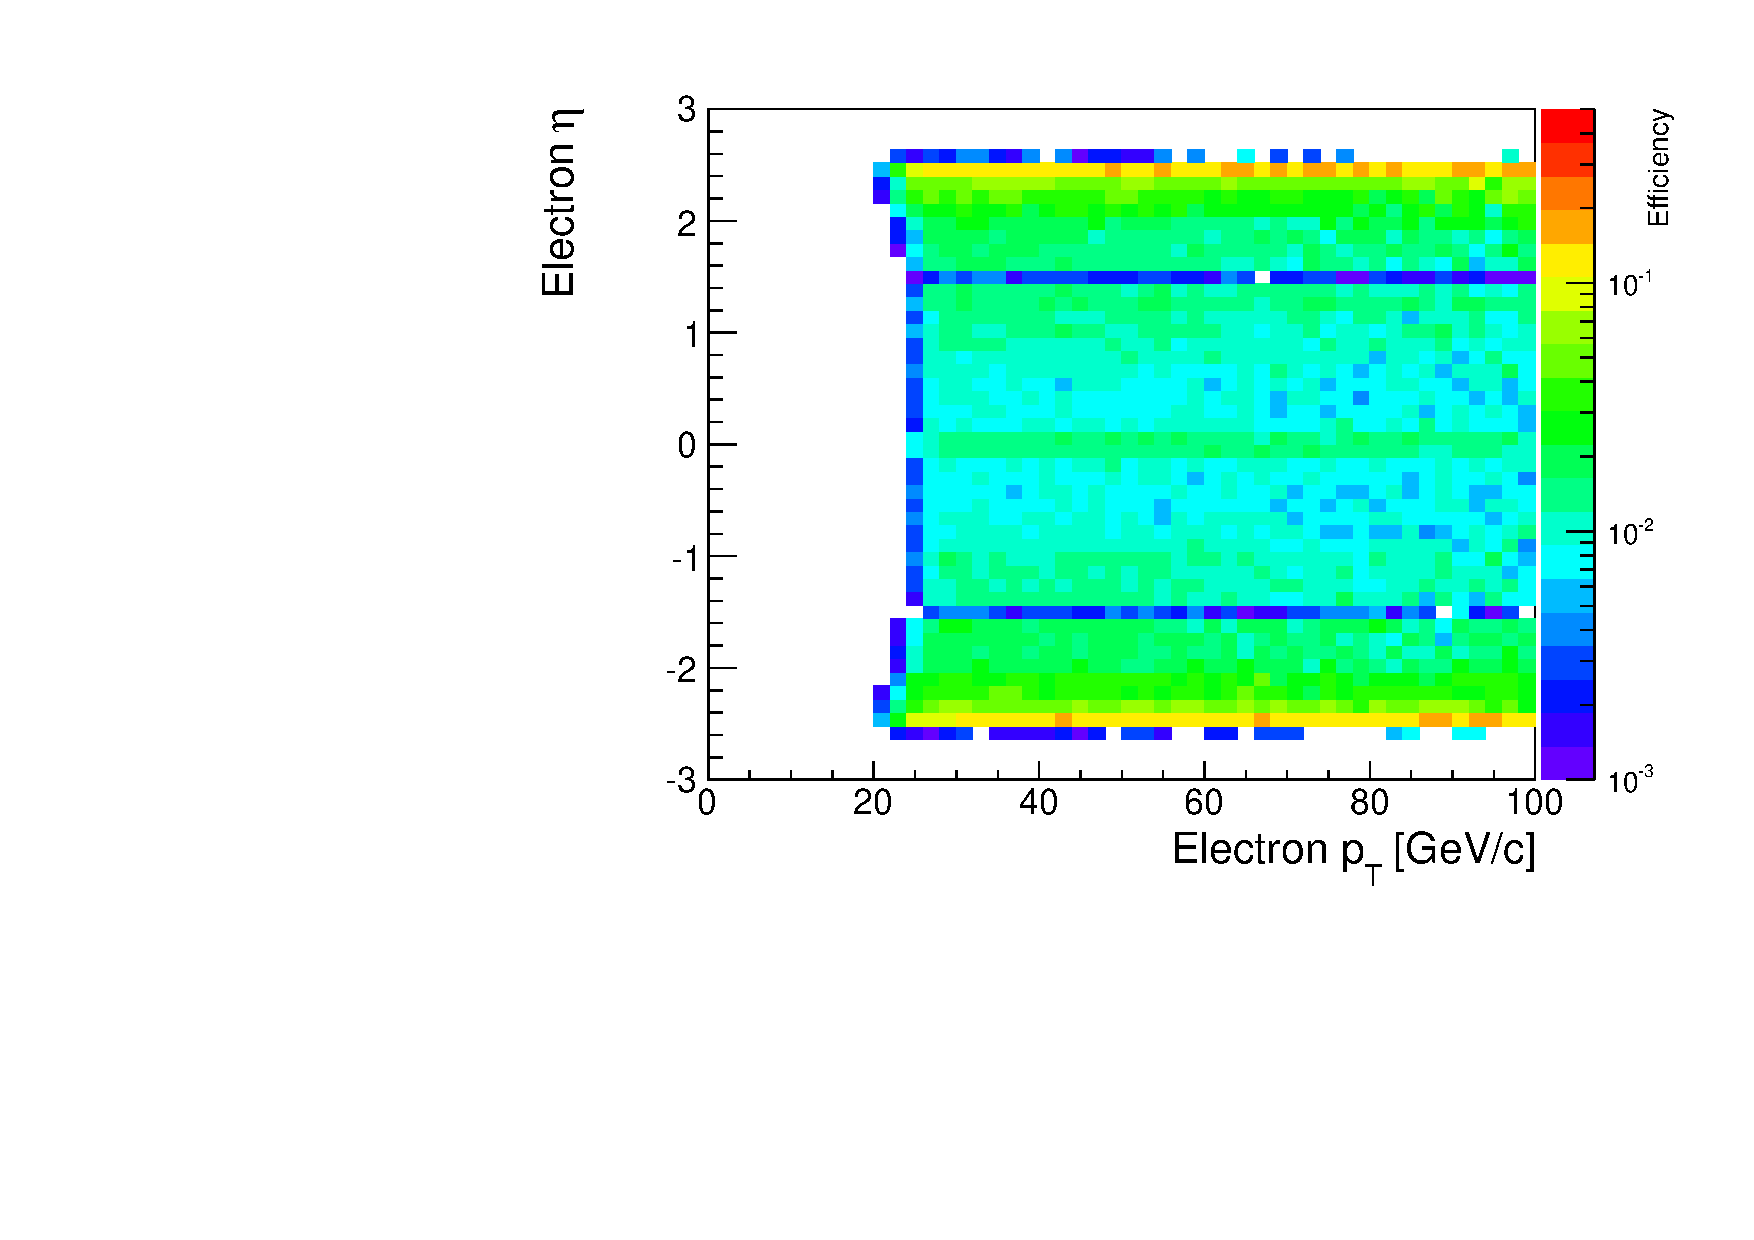
\includegraphics[width=0.9\textwidth]{figures/EfficiencyPtEta_ElectronFakesPhoton.pdf}
  \caption{Electron To Photon Fake Rate}
  \label{fig:electronToPhotonFakerate}
\end{figure}


\subsection{Summary of Backgrounds}

Combining estimates of all background processes together, we show 
a stacked histogram of the diphoton mass and the di-bjet mass distributions
in Figures \ref{fig:DiPhotonMass_AfterObjectSelection} and 
\ref{fig:DiBJetMass_AfterObjectSelection} after the object selection. In Figure 
\ref{fig:DRVariables_AfterObjectSelection} we show the distributions of the $\Delta \mathrm{R}_{\gamma\gamma}$
between the two photons, and the minimum $\Delta$R between any photon and any b-jet.
The distributions of the $p_{T}$ of the diphoton and di-bjet systems are shown in 
Figures \ref{fig:pTVariables_AfterObjectSelection}. Finally, we show the 
diphoton and di-bjet mass distributions after making selection requirements on 
the $\Delta$R variables as described in Section \ref{} in 
Figures \ref{fig:DiPhotonMass_AfterKinematicSelection}
and \ref{fig:DiBJetMass_AfterKinematicSelection}. 


%% \begin{figure}[h]
%%   \centering
%% %  \includegraphics[width=0.9\textwidth]{figures/DiPhotonMass_AfterObjectSelection.pdf}
%%   \caption{DiPhotonMass_AfterObjectSelection}
%%   \label{fig:DiPhotonMass_AfterObjectSelection}
%% \end{figure}

%% \begin{figure}[h]
%%   \centering
%% %  \includegraphics[width=0.9\textwidth]{figures/DiBJetMass_AfterObjectSelection.pdf}
%%   \caption{DiBJetMass_AfterObjectSelection}
%%   \label{fig:DiBJetMass_AfterObjectSelection}
%% \end{figure}

%% \begin{figure}[h]
%%   \centering
%% %  \includegraphics[width=0.45\textwidth]{figures/DRgg_AfterObjectSelection.pdf}
%% %  \includegraphics[width=0.45\textwidth]{figures/minDRgb_AfterObjectSelection.pdf}
%%   \caption{DRVariables_AfterObjectSelection}
%%   \label{fig:DRVariables_AfterObjectSelection}
%% \end{figure}

%% \begin{figure}[h]
%%   \centering
%% %  \includegraphics[width=0.45\textwidth]{figures/pTgg_AfterObjectSelection.pdf} 
%% %  \includegraphics[width=0.45\textwidth]{figures/ptbb_AfterObjectSelection.pdf}
%%   \caption{pTVariables_AfterObjectSelection}
%%   \label{fig:pTVariables_AfterObjectSelection}
%% \end{figure}

%% \begin{figure}[h]
%%   \centering
%% %  \includegraphics[width=0.9\textwidth]{figures/DiPhotonMass_AfterKinematicSelection.pdf}
%%   \caption{DiPhotonMass_AfterKinematicSelection}
%%   \label{fig:DiPhotonMass_AfterKinematicSelection}
%% \end{figure}
%% \begin{figure}[h]
%%   \centering
%% %  \includegraphics[width=0.9\textwidth]{figures/DiBJetMass_AfterKinematicSelection.pdf}
%%   \caption{DiBJetMass_AfterKinematicSelection}
%%   \label{fig:DiBJetMass_AfterKinematicSelection}
%% \end{figure}


To show a rough estimate of the sensitivity of a cut-based analysis, we
summarize the signal and background event yields in 
Tables \ref{tab:EventYieldSummaryConservativeMassWindows}
and \ref{tab:EventYieldSummaryOptimisticMassWindows} 
for two sets of mass window selection cuts, one assuming
conservative estimates of resolution performance ( $120 < M_{\gamma\gamma} < 130$ and 
 $105 < M_{bb} < 145$ ) , and one assuming a more optimistic resolution
performance ($122 < M_{\gamma\gamma} < 128$ and  $100 < M_{bb} < 140$ ).



\begin{table}[!ht]
\begin{center} 
\begin{tabular}{|c|c|}
\hline 
Process                                              &  Event Yield at $3$~$ab^{-1}$ \\  \hline
$HH \rightarrow bb\gamma\gamma$ (Signal)             &  00000                     \\  \hline
$ZH \rightarrow b\bar{b}\gamma\gamma$                &  00000                     \\  
$t\bar{t}H \rightarrow W W b \bar{b}\gamma\gamma$    &  00000                     \\  \hline
$b \bar{b} \gamma\gamma$                             &  00000                     \\  
$jj \gamma\gamma$ (Mistags)                          &  00000                     \\  
$bb jj$ (Fake Photons)                               &  00000                     \\  
$cc jj$ (Fake Photons \& Mistags)                    &  00000                     \\  
$jjjj$  (Fake Photons \& Mistags)                    &  00000                     \\  \hline
$t\bar{t}$ (Electron Fakes Photons)                  &  00000                     \\  \hline
\hline
$S/B$                                                &  00000                     \\  \hline
$S/\sqrt{B}$                                         &  00000                     \\  \hline

\end{tabular}
\caption{Expected Yields for conservative mass windows }
\label{tab:EventYieldSummaryConservativeMassWindows}
\end{center}
\end{table}
 

\begin{table}[!ht]
\begin{center} 
\begin{tabular}{|c|c|}
\hline 
Process                                              &  Event Yield at $3$~$ab^{-1}$ \\  \hline
$HH \rightarrow bb\gamma\gamma$ (Signal)             &  00000                     \\  \hline
$ZH \rightarrow b\bar{b}\gamma\gamma$                &  00000                     \\  
$t\bar{t}H \rightarrow W W b \bar{b}\gamma\gamma$    &  00000                     \\  \hline
$b \bar{b} \gamma\gamma$                             &  00000                     \\  
$jj \gamma\gamma$ (Mistags)                          &  00000                     \\  
$bb jj$ (Fake Photons)                               &  00000                     \\  
$cc jj$ (Fake Photons \& Mistags)                    &  00000                     \\  
$jjjj$  (Fake Photons \& Mistags)                    &  00000                     \\  \hline
$t\bar{t}$ (Electron Fakes Photons)                  &  00000                     \\  \hline
\hline
$S/B$                                                &  00000                     \\  \hline
$S/\sqrt{B}$                                         &  00000                     \\  \hline

\end{tabular}
\caption{Expected Yields for optimistic mass windows }
\label{tab:EventYieldSummaryOptimisticMassWindows}
\end{center}
\end{table}
 


\section{Signal Extraction}
\label{sec:signalextraction}

We present three analysis methods for extracting the signal and its cross section, with increasing
level of complexity. The first method is a ``cut and count'' method where we apply
the event selection requirements outlined in Section \ref{sec:eventselection}, 
and count the event yield, subtracting the estimates of the expected background. From Tables
\ref{tab:EventYieldSummaryConservativeMassWindows} and \ref{tab:EventYieldSummaryOptimisticMassWindows}
we expect total event yields of $XX$ and $XX$ for the conservative and optimistic mass window scenarios
and a corresponding relative uncertainty on the signal yield of $XX\%$ and $XX\%$, respectively.

The second analysis method applies the selection cuts for ``Scheme1'' from section \ref{}, applies
a conservative window on the diphoton mass from $120$~GeV to $130$~GeV, and performs a maximum
likelihood fit on the di-bjet mass distribution. Finally, the third analysis method, applies
the selection cuts for ``Scheme1'' and a two dimensional maximum likelihood fit is performed
on the diphoton and di-bjet mass distributions.

\subsection{Maximum Likelihood Mass Fits}
\label{sec:massfits}

We derive probability density functions (PDF's) for the diphoton mass, $m_{\gamma\gamma}$, and di-bjet mass, $m_{bb}$
 distributions for the signal, the resonant background, and the non-resonant background by 
fitting the distributions from the Monte Carlo simulation samples to particular parameterizations 
of the lineshape for $m_{\gamma\gamma}$ and $m_{bb}$. The $m_{\gamma\gamma}$
distribution of the signal and resonant background is fitted to a Gaussian distribution, while for
the non-resonant background it is fitted to a decaying exponential. The $m_{bb}$ distribution 
for the signal and resonant backgrounds, dominated by ZH where the Z boson decays into a pair of b-jets,
are fitted to a Crystal Ball distribution. The $m_{bb}$ distribution for the non-resonant background is
again fitted to a decaying exponential. Figure \ref{fig:TwoDFitModels} shows the $m_{\gamma\gamma}$
and $m_{bb}$ distributions and PDF's used to model the lineshape for the signal, the resonant background,
and the non-resonant background.

\begin{figure}[h!]
  \centering
  \subfigure[]{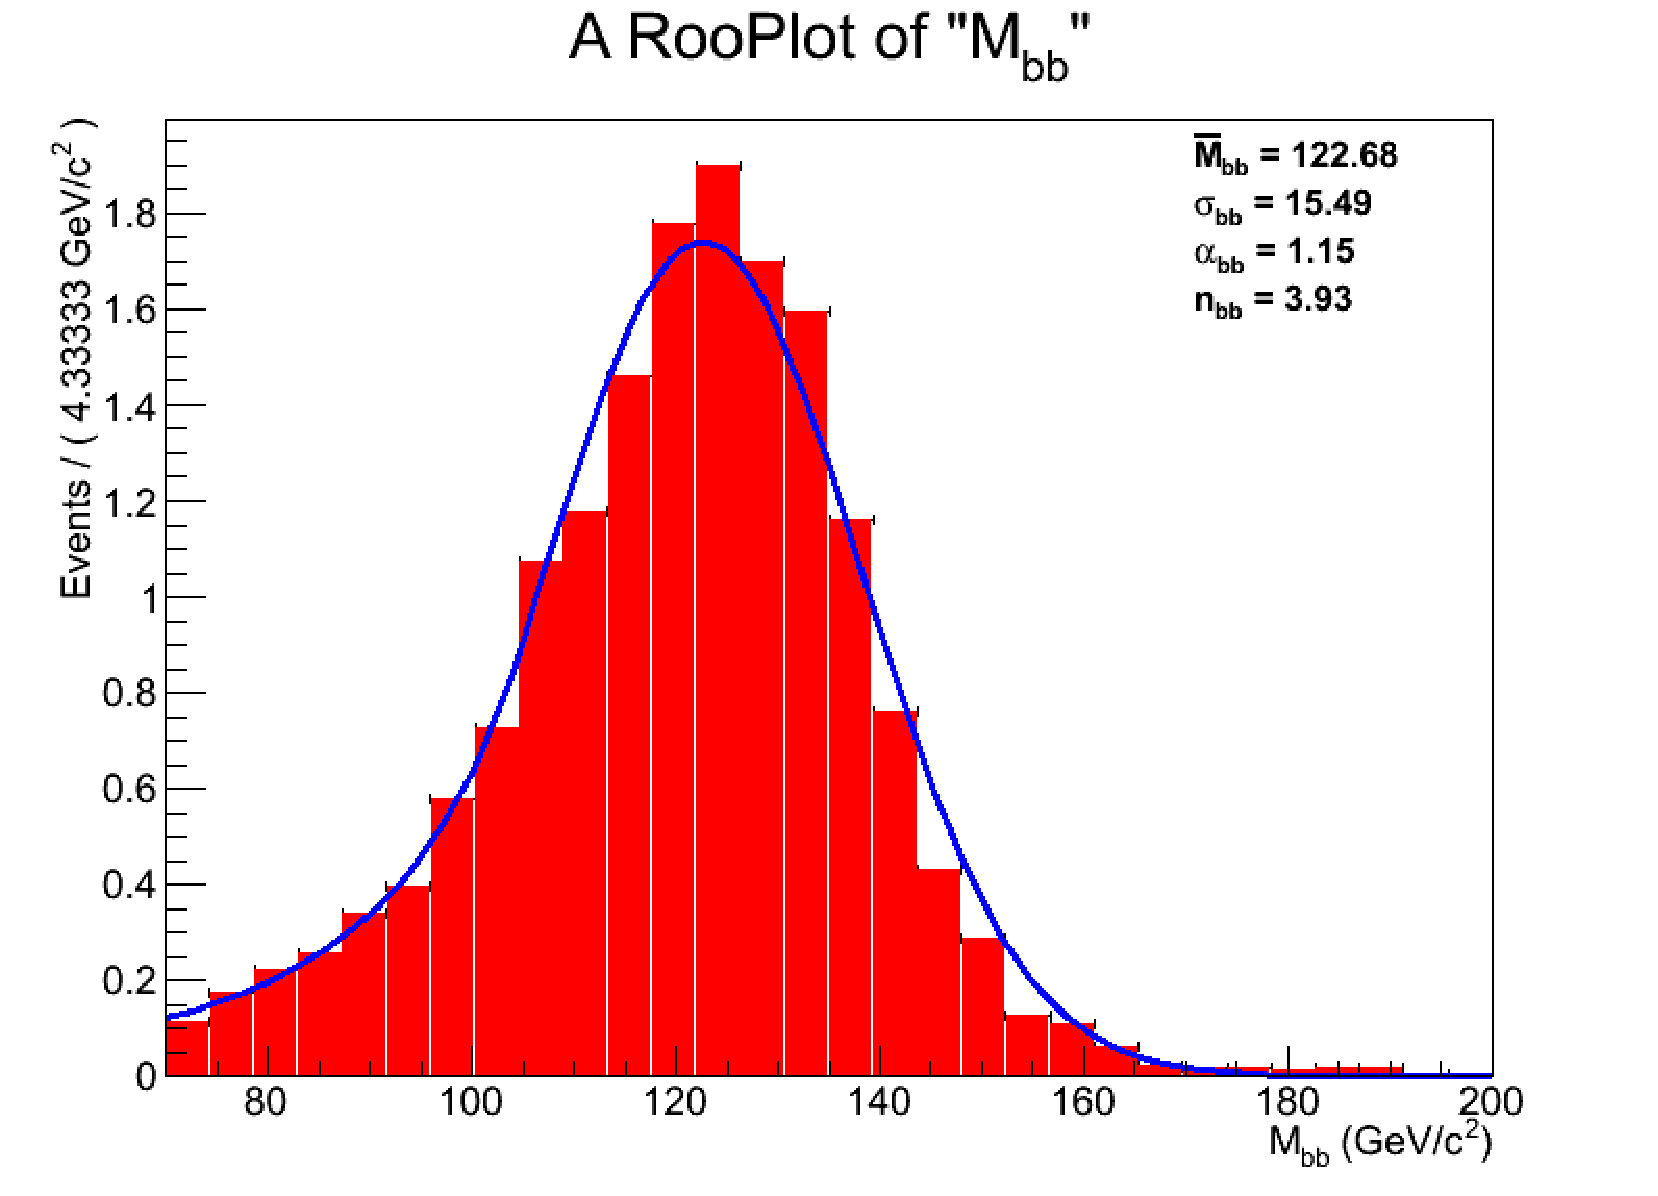
\includegraphics[width=0.32\textwidth]{figures/sigBjetHistFitCB.pdf}}
  \subfigure[]{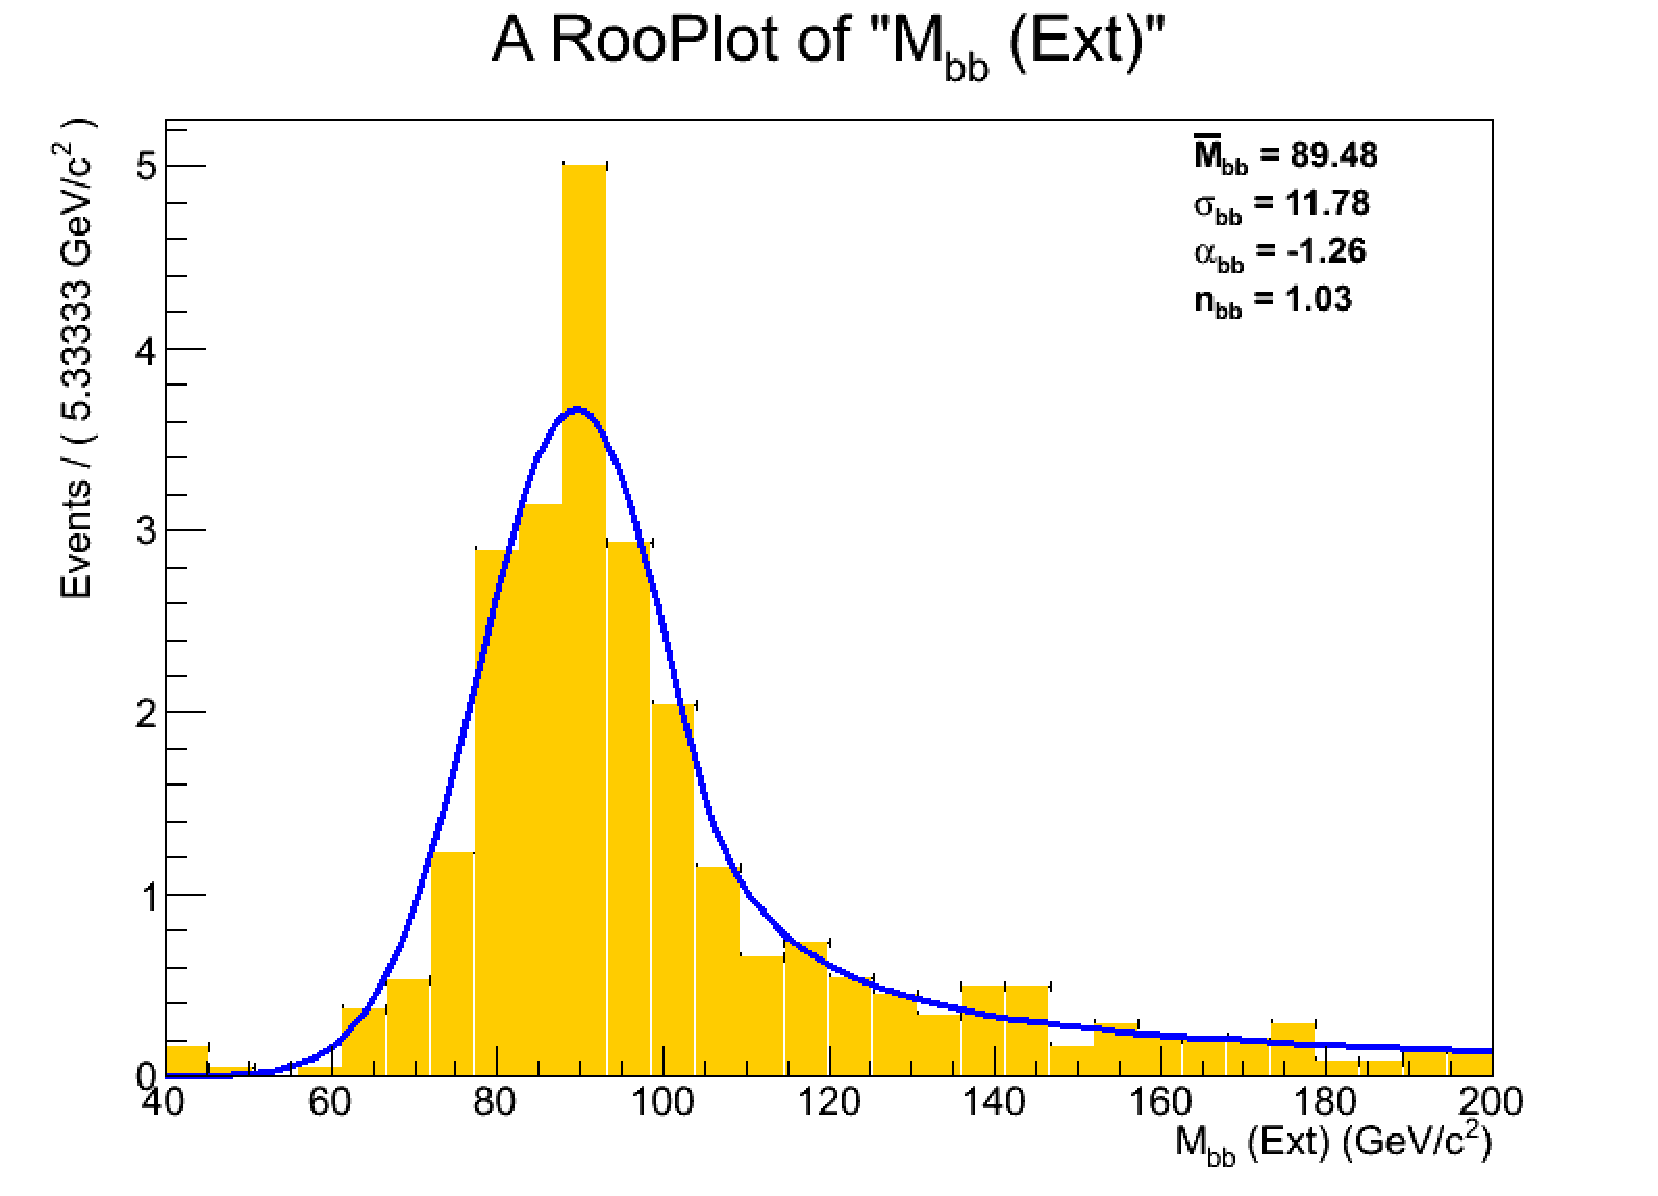
\includegraphics[width=0.32\textwidth]{figures/resBjetHistExtFitCB.pdf}}
  \subfigure[]{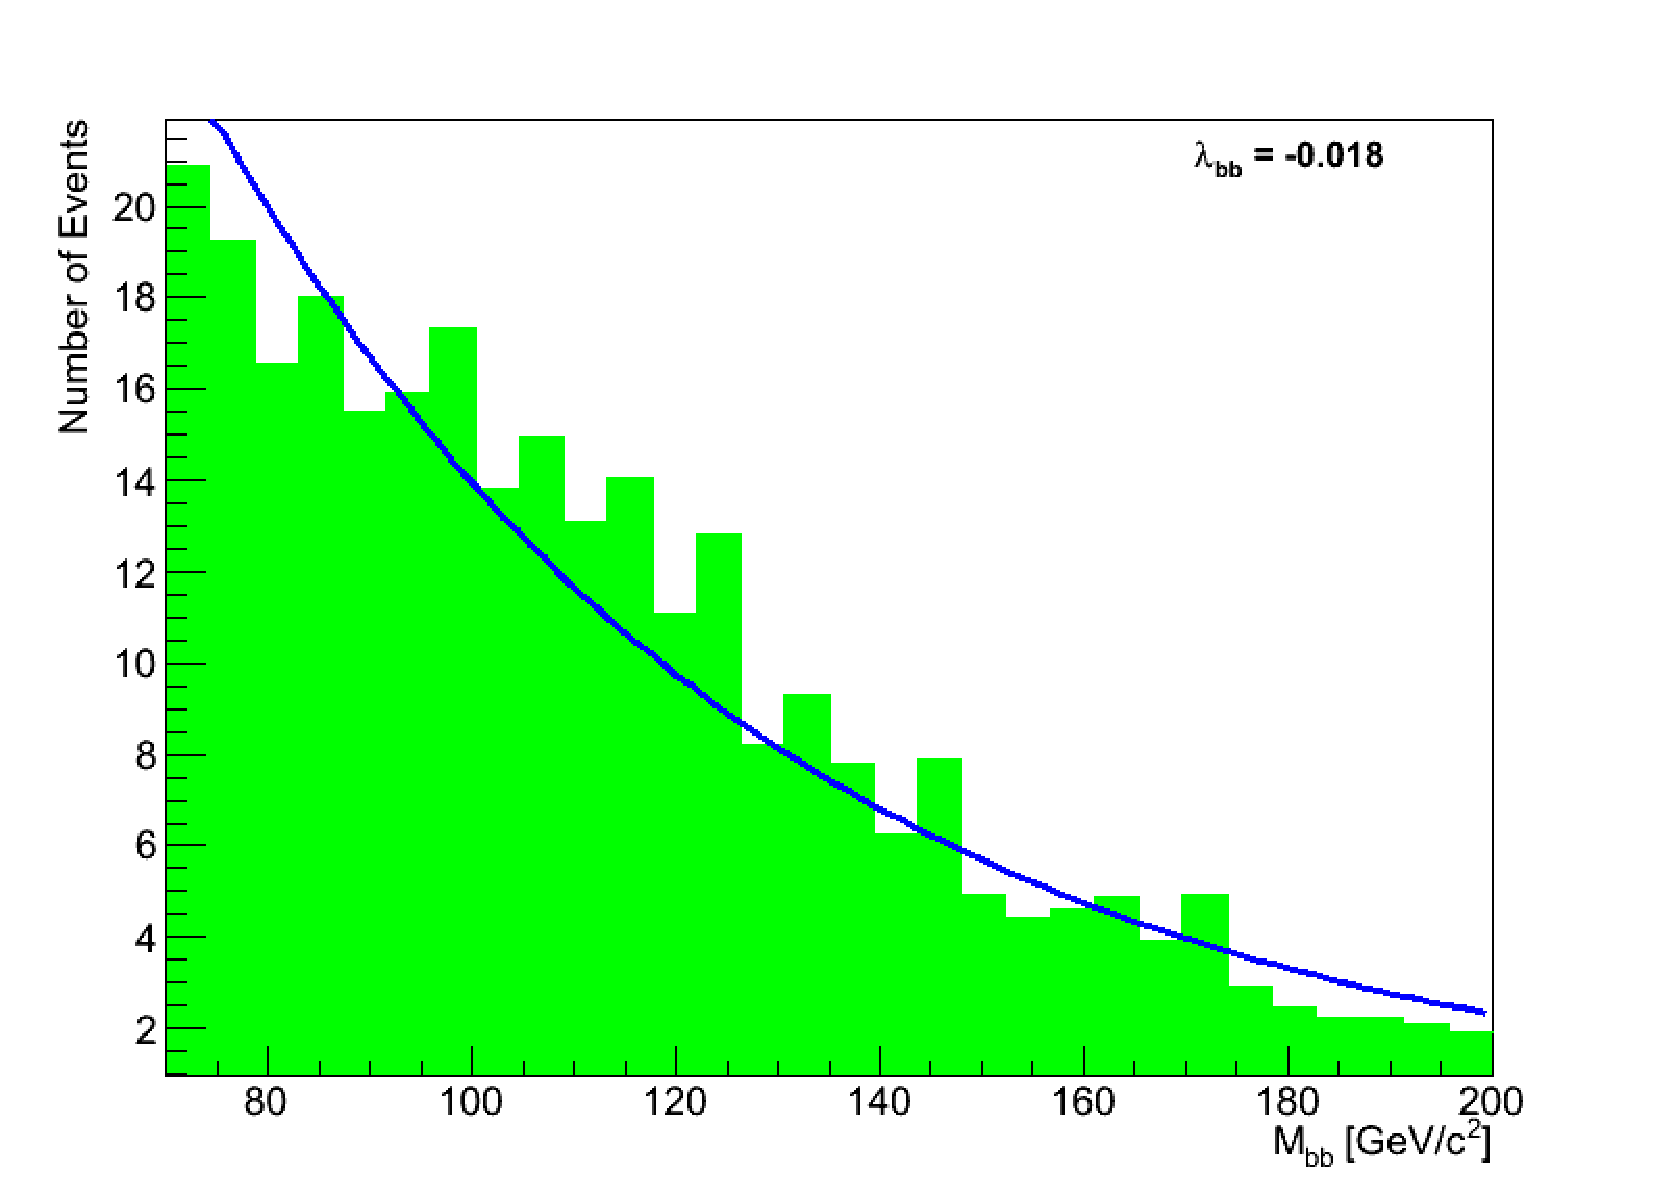
\includegraphics[width=0.32\textwidth]{figures/nonresBjetHistFitExpo.pdf}}
  \subfigure[]{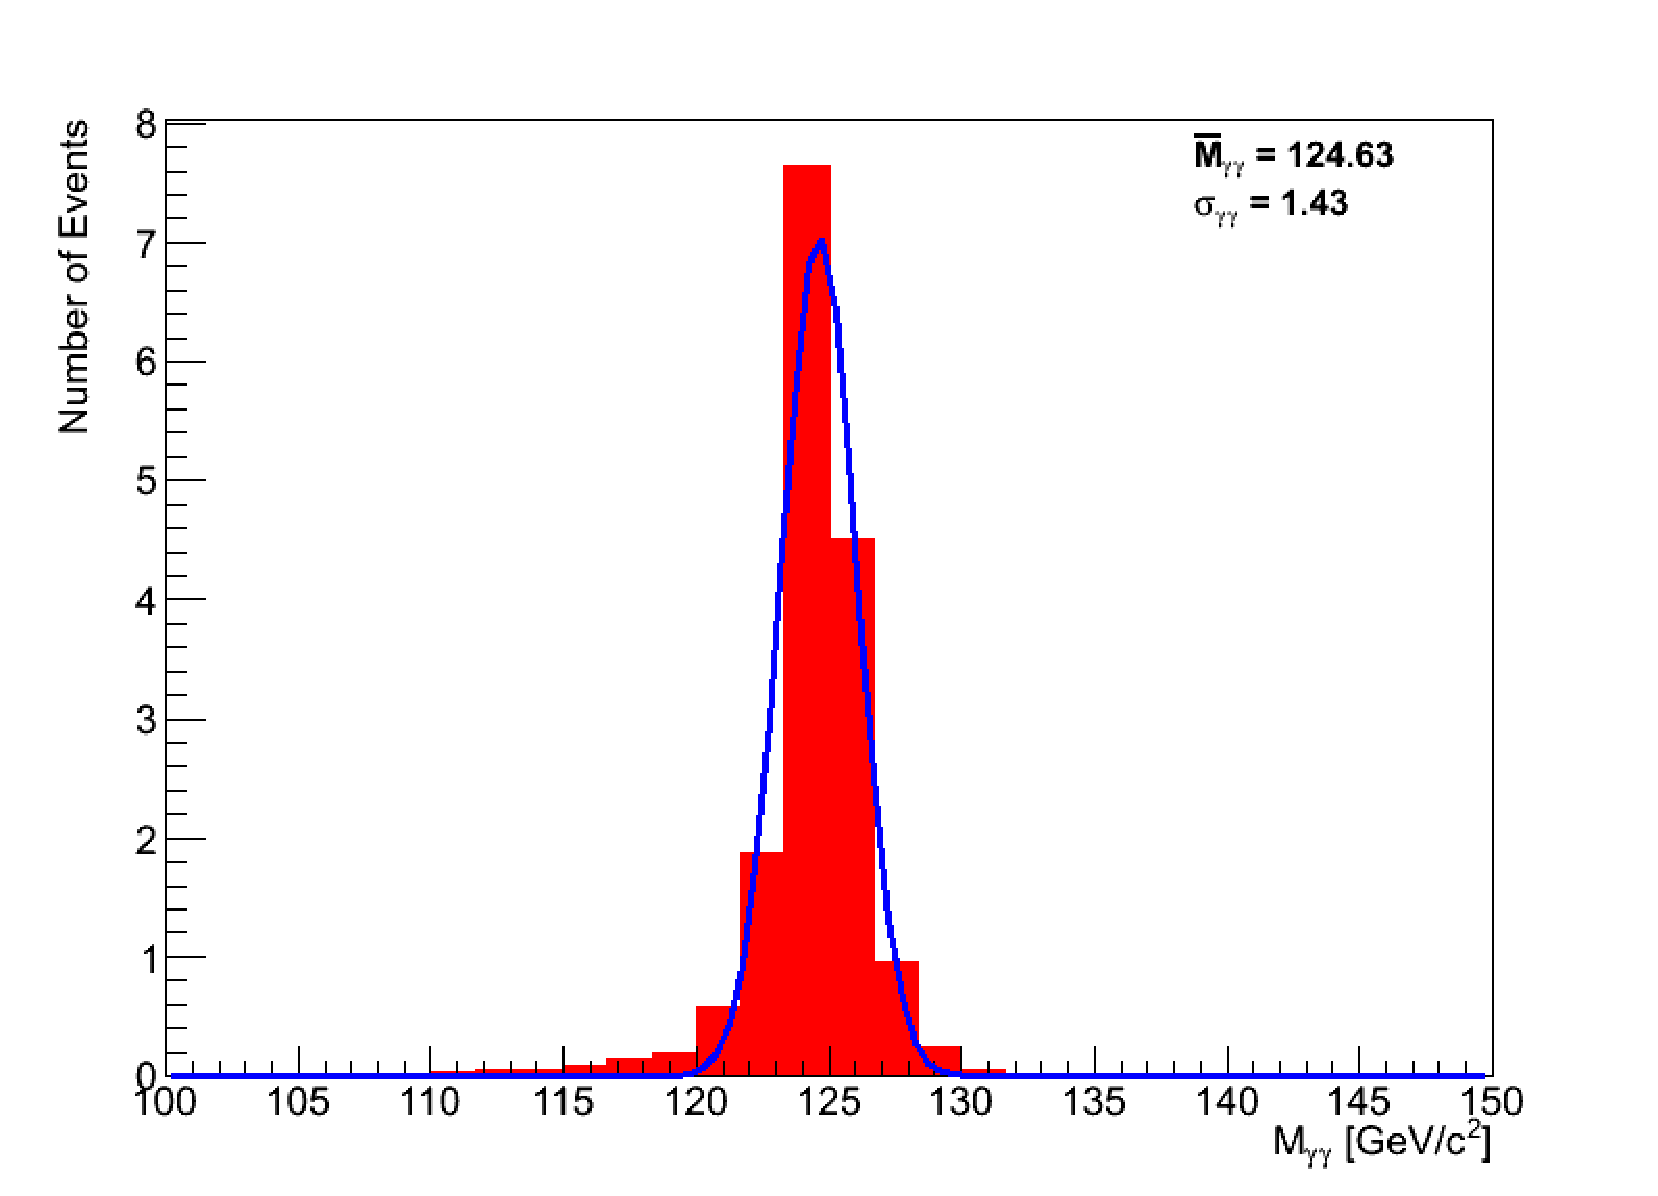
\includegraphics[width=0.32\textwidth]{figures/sigPhoHistFit.pdf}}
  \subfigure[]{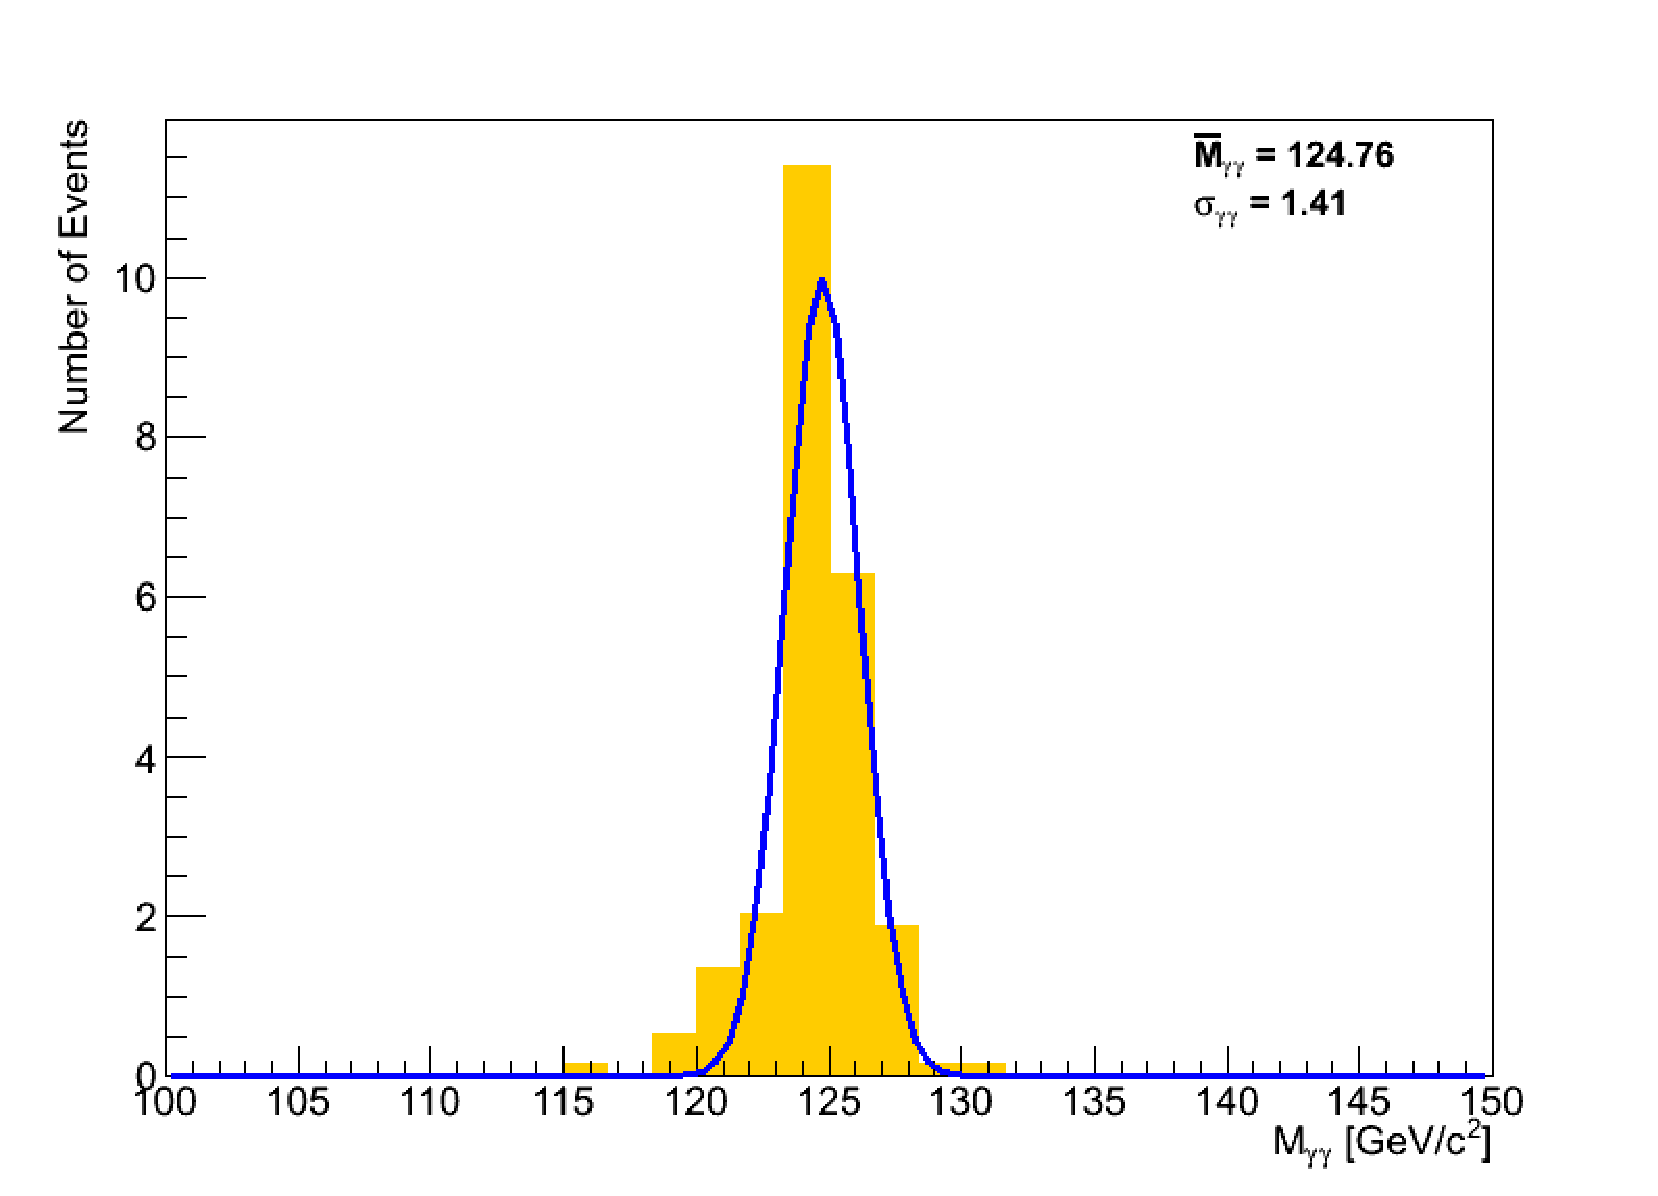
\includegraphics[width=0.32\textwidth]{figures/resPhoHistFit.pdf}}
  \subfigure[]{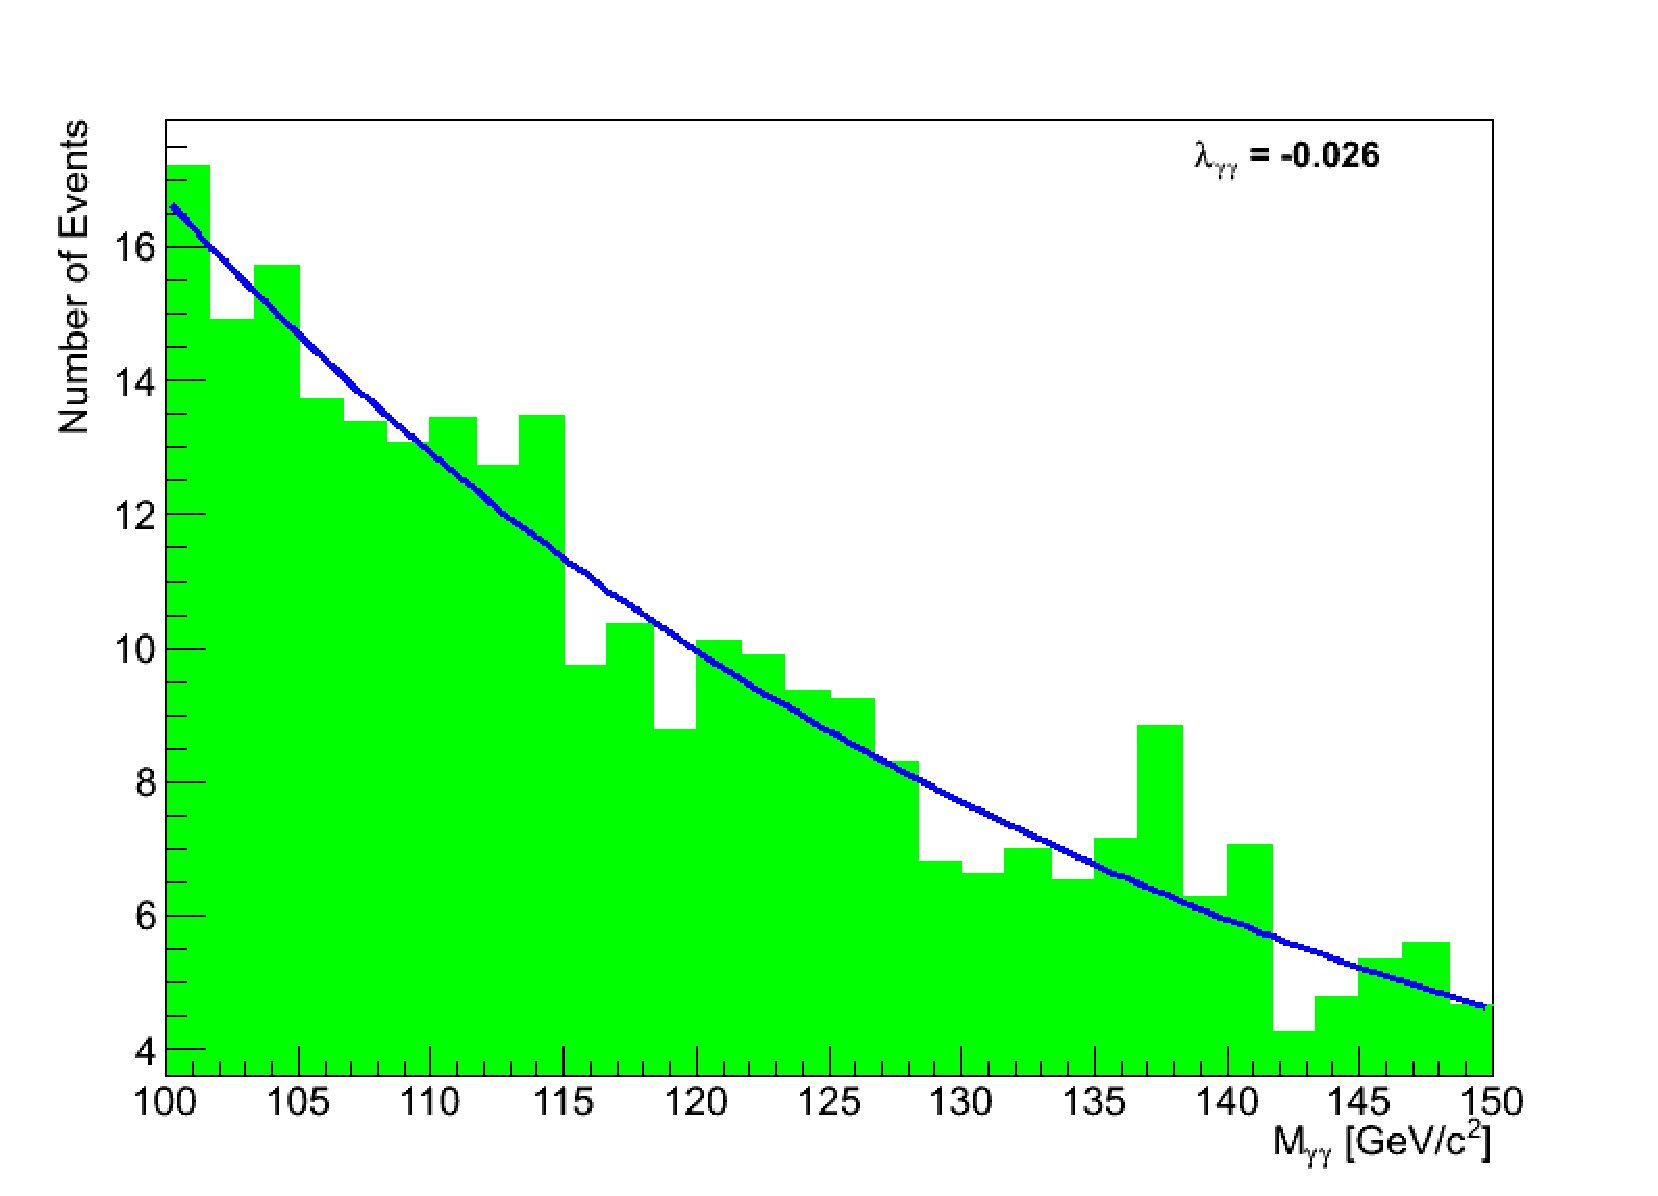
\includegraphics[width=0.32\textwidth]{figures/nonresPhoHistFitExpo.pdf}}
  \caption{The preliminary fits of (a) the signal, (b) resonant background, and (c) non-resonant background on the di-bjet mass distribution and the preliminary fits of (d) the signal, (e) resonant background, and (f) non-resonant background on the diphoton mass distribution.}
  \label{fig:prelimTwoDFits}
\end{figure}

We check for correlations between $m_{\gamma\gamma}$ and $m_{bb}$ by evaluating the correlation coefficient
for the three different background components, and find values of $0.016$ for the signal, 
$0.060$ for the resonant background, and $0.059$ for the non-resonant background. These values are sufficiently
close to zero that we assume no correlation between the two masses. Therefore, the two 
dimensional PDF's are simply the product of the one dimensional PDF's.


\subsubsection{One Dimensional Fits}
We first perform a one dimensional maximum likelihood fit on the di-bjet mass distribution. 
The selection cuts labelled ``Scheme1'' from Section \ref{sec:eventselection} are applied, and a conservative
window on the diphoton mass from $120$~GeV to $130$~GeV is required to reduce non-resonant background. 
Using the expected event yields for the signal, resonant background, and non-resonant background, as
weights, we combine the PDF's for the three different processes into a total PDF to model the full
signal region sample.

Toy Monte Carlo experiments are generated randomly from this model, and the pseudodata are fitted
to this model, where the event yields for the signal, the resonant background, and the non-resonant
background are allowed to float, as well as the parameters of the exponential function modelling
the non-resonant background. One example toy experiment and fitted result is shown in 
Figure \ref{fig:oneDfullFit}. 

Figure \ref{fig:oneDpullPlot} summarizes the pull distribution for a set of 10,000 toy MC experiments,
illustrating that there is essentially no bias in the fitting procedure. We show also the
distribution of the relative fit uncertainty on the signal yield, representing an estimate of the
statistical uncertainty of the cross section measurement. 

\begin{figure}[h]
  \centering
  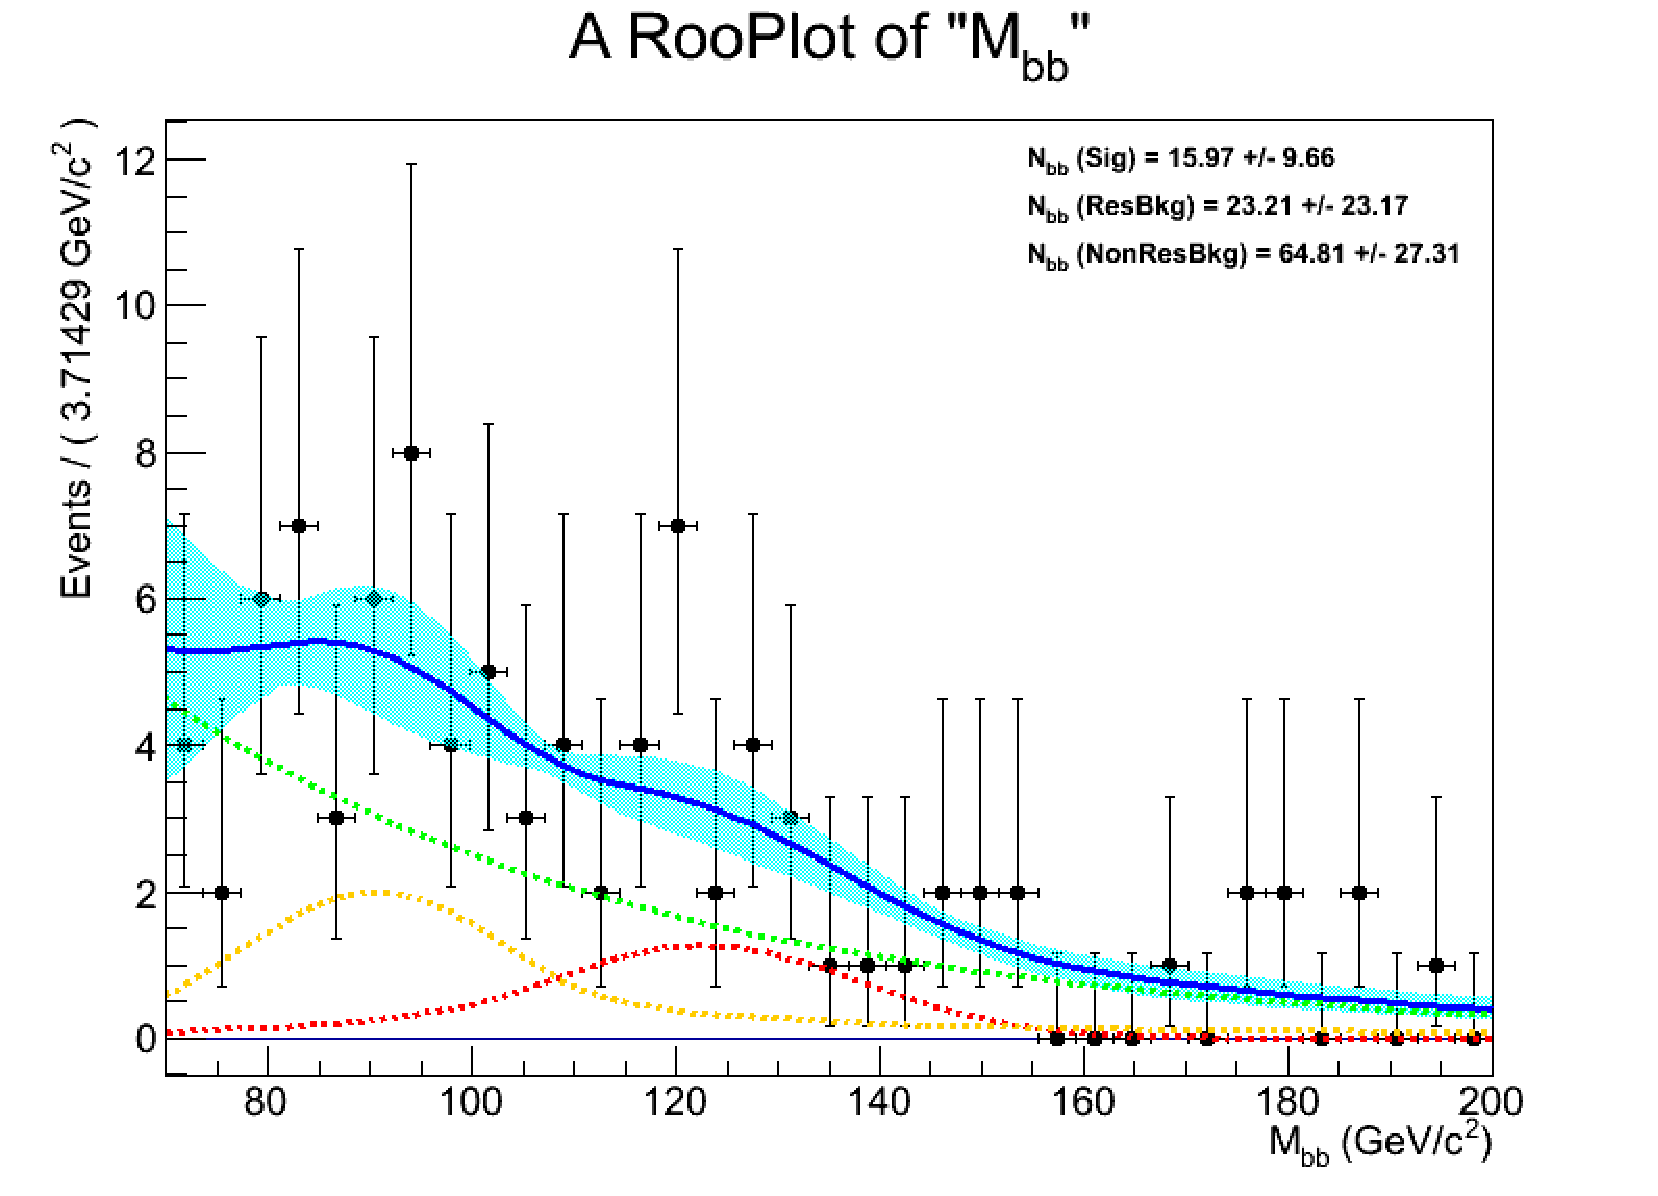
\includegraphics[width=0.9\textwidth]{figures/oneDimFitPhoWin_0.pdf}
  \caption{Example of a full one dimensional fit on the di-bjet mass. The signal, resonant background, and non-resonant background components are respectively shown in red, yellow, and green.}
  \label{fig:oneDfullFit}
\end{figure}

\begin{figure}[h]
  \centering
  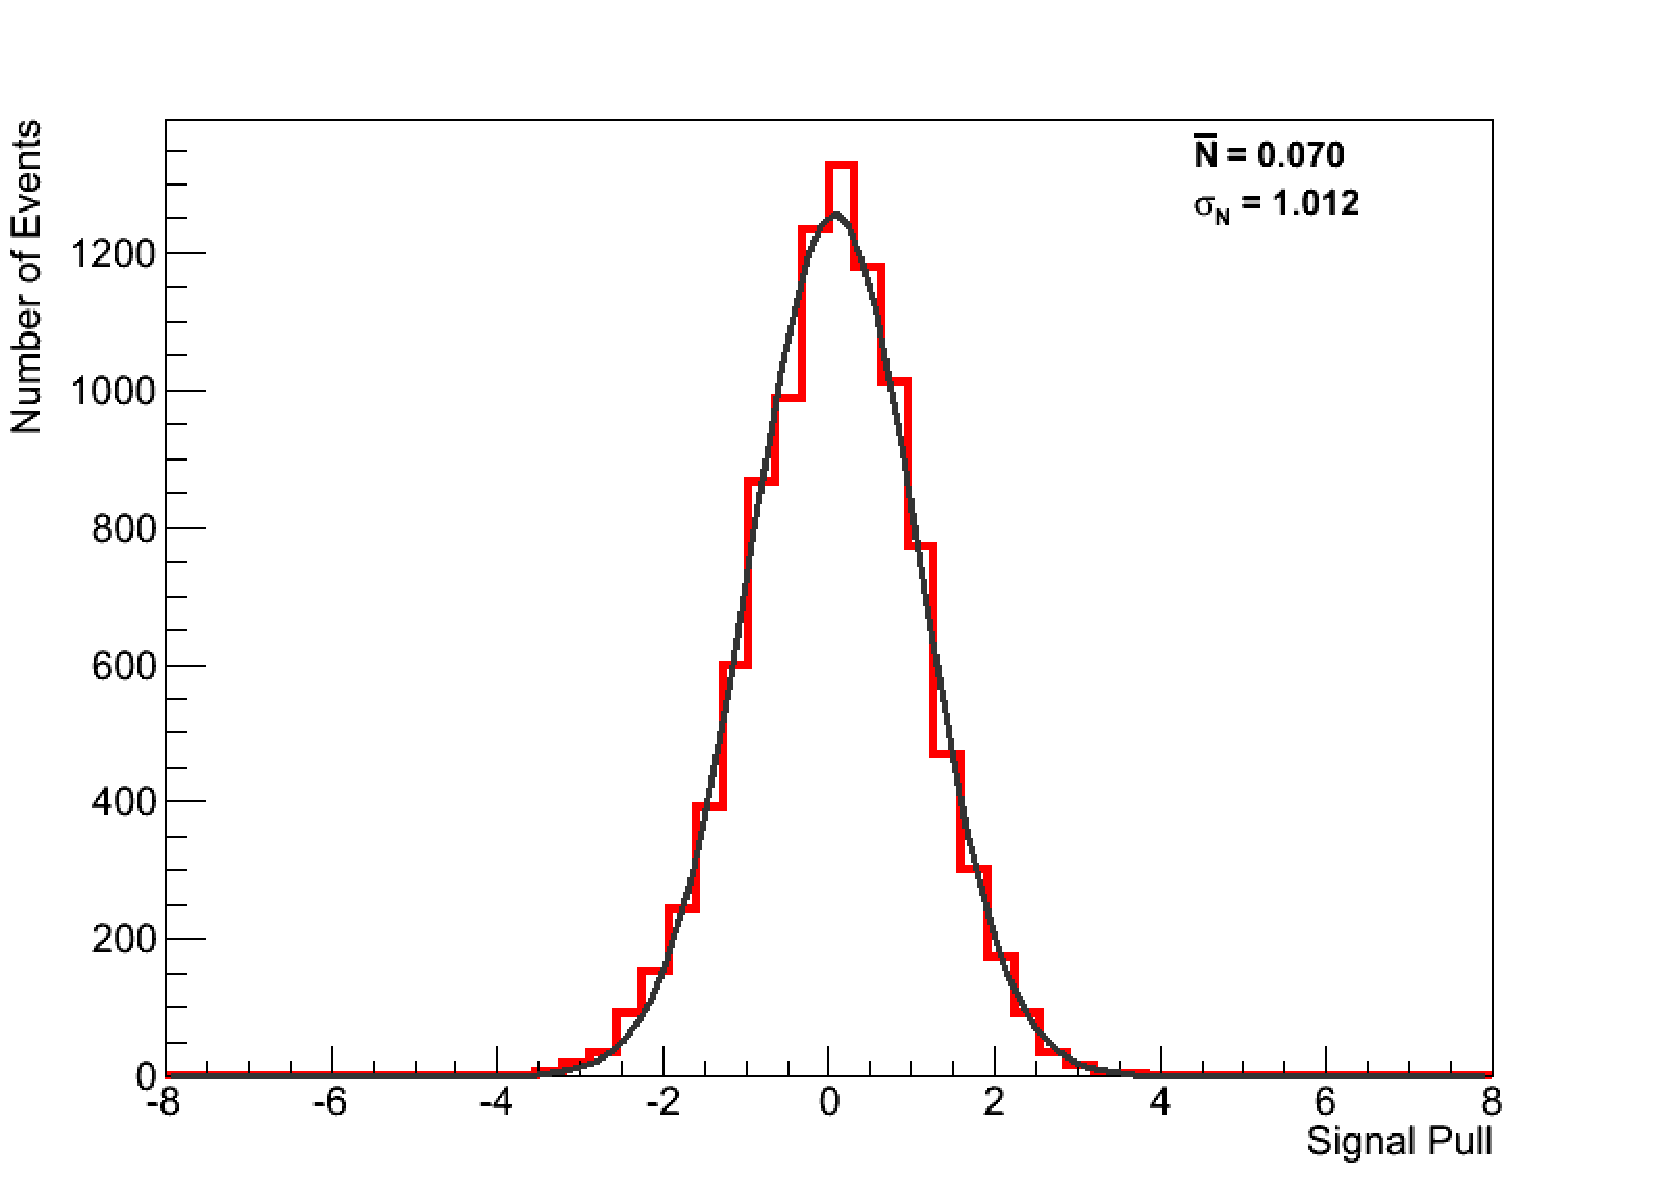
\includegraphics[width=0.45\textwidth]{figures/sigPullFitOneD.pdf}
  %\includegraphics[width=0.45\textwidth]{figures/relativeErrFitOneD.pdf}
  \caption{Pull distribution and Gaussian fit for 10,000 one dimensional toy MC experiments.}
  \label{fig:oneDfullFit}
\end{figure}

\subsubsection{Two Dimensional Fits}
Finally, we perform a two dimensional maximum likelihood fit to the diphoton mass and di-bjet mass distributions. 
We apply again the ``Scheme1'' selection requirements, and apply wide mass windows from $100$~GeV to $150$~GeV
for the diphoton mass, and from $70$~GeV to $200$~GeV for the di-bjet mass. The expected number of events
are used to weight the PDF's for the signal, the resonant background, and the non-resonant background to build
the model for the signal region sample. 

We perform, again, toy Monte Carlo experiments randomly drawn from the full model and perform the two dimensional
fit, where we float the yields of the signal, the resonant background, and the non-resonant background, as well as
the parameters of the exponential function modelling the non-resonant background. Figure \ref{fig:twoDfullFit}
shows one example toy experiment and the fitted result. In Figure \ref{fig:twoDpullPlot},
we show the pull distribution for a sample of 10,000 toy MC experiments, demonstrating that the fit yields unbiased
measurements of the signal yield and its uncertainty. We show also the distribution of the fit uncertainty
on the signal yield, showing the average statistical uncertainty of the cross section measurement using the two
dimensional fit. In Table \ref{tab:RelativeUncertaintyOnSignalYield},
we compare the average statistical uncertainty on the cross section measurement
for the cut-based analysis, the one dimensional fit to $m_{bb}$, and the two dimensional fit. 

\begin{figure}[h]
  \centering
  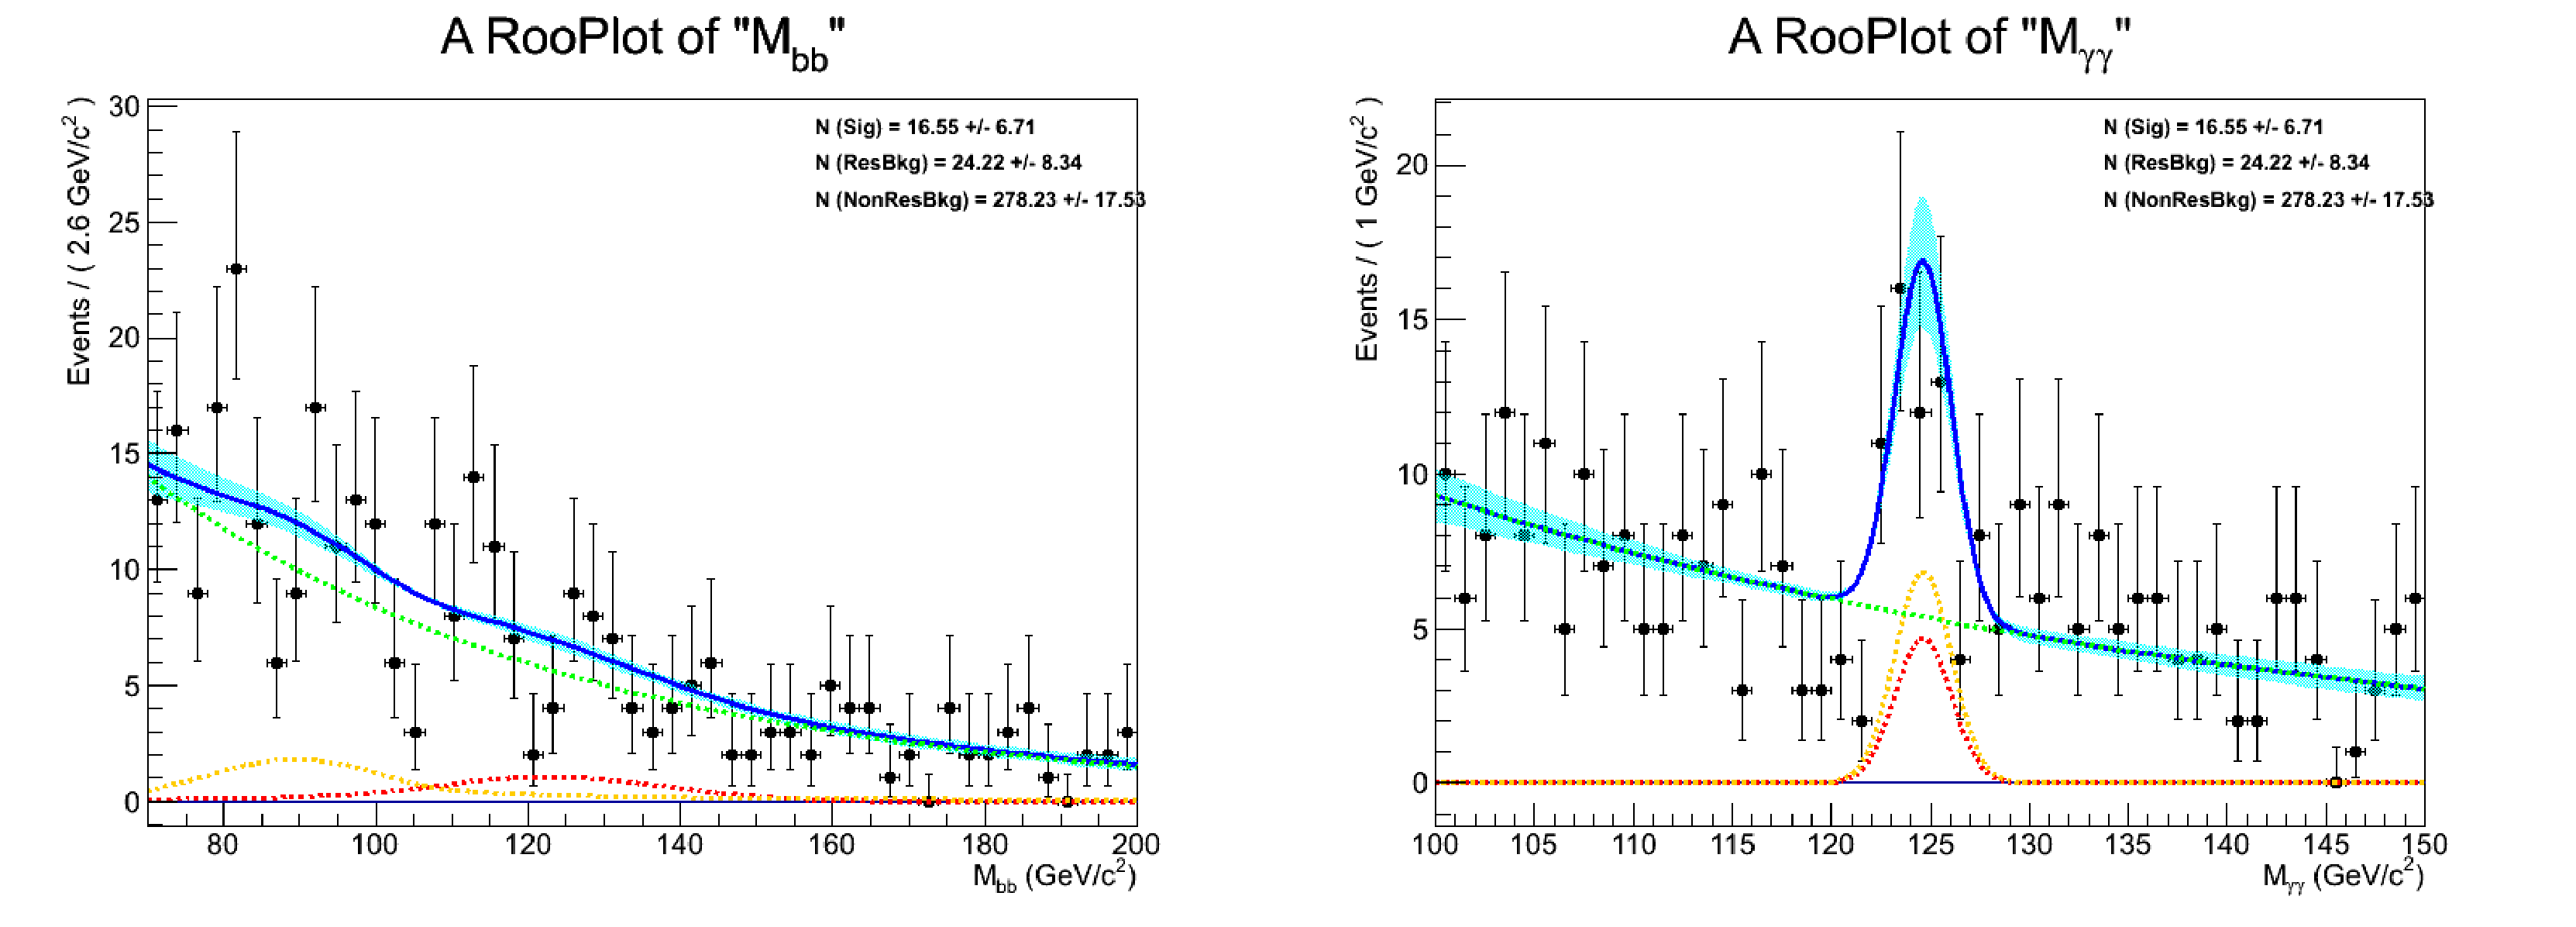
\includegraphics[width=0.9\textwidth]{figures/projectionFits_0.pdf}
  \caption{Projections of a full two dimensional fit on the di-bjet mass (left) and diphoton mass (right). The signal, resonant background, and non-resonant background components are respectively shown in red, yellow, and green.}
  \label{fig:twoDfullFit}
\end{figure}


\begin{figure}[h]
  \centering
  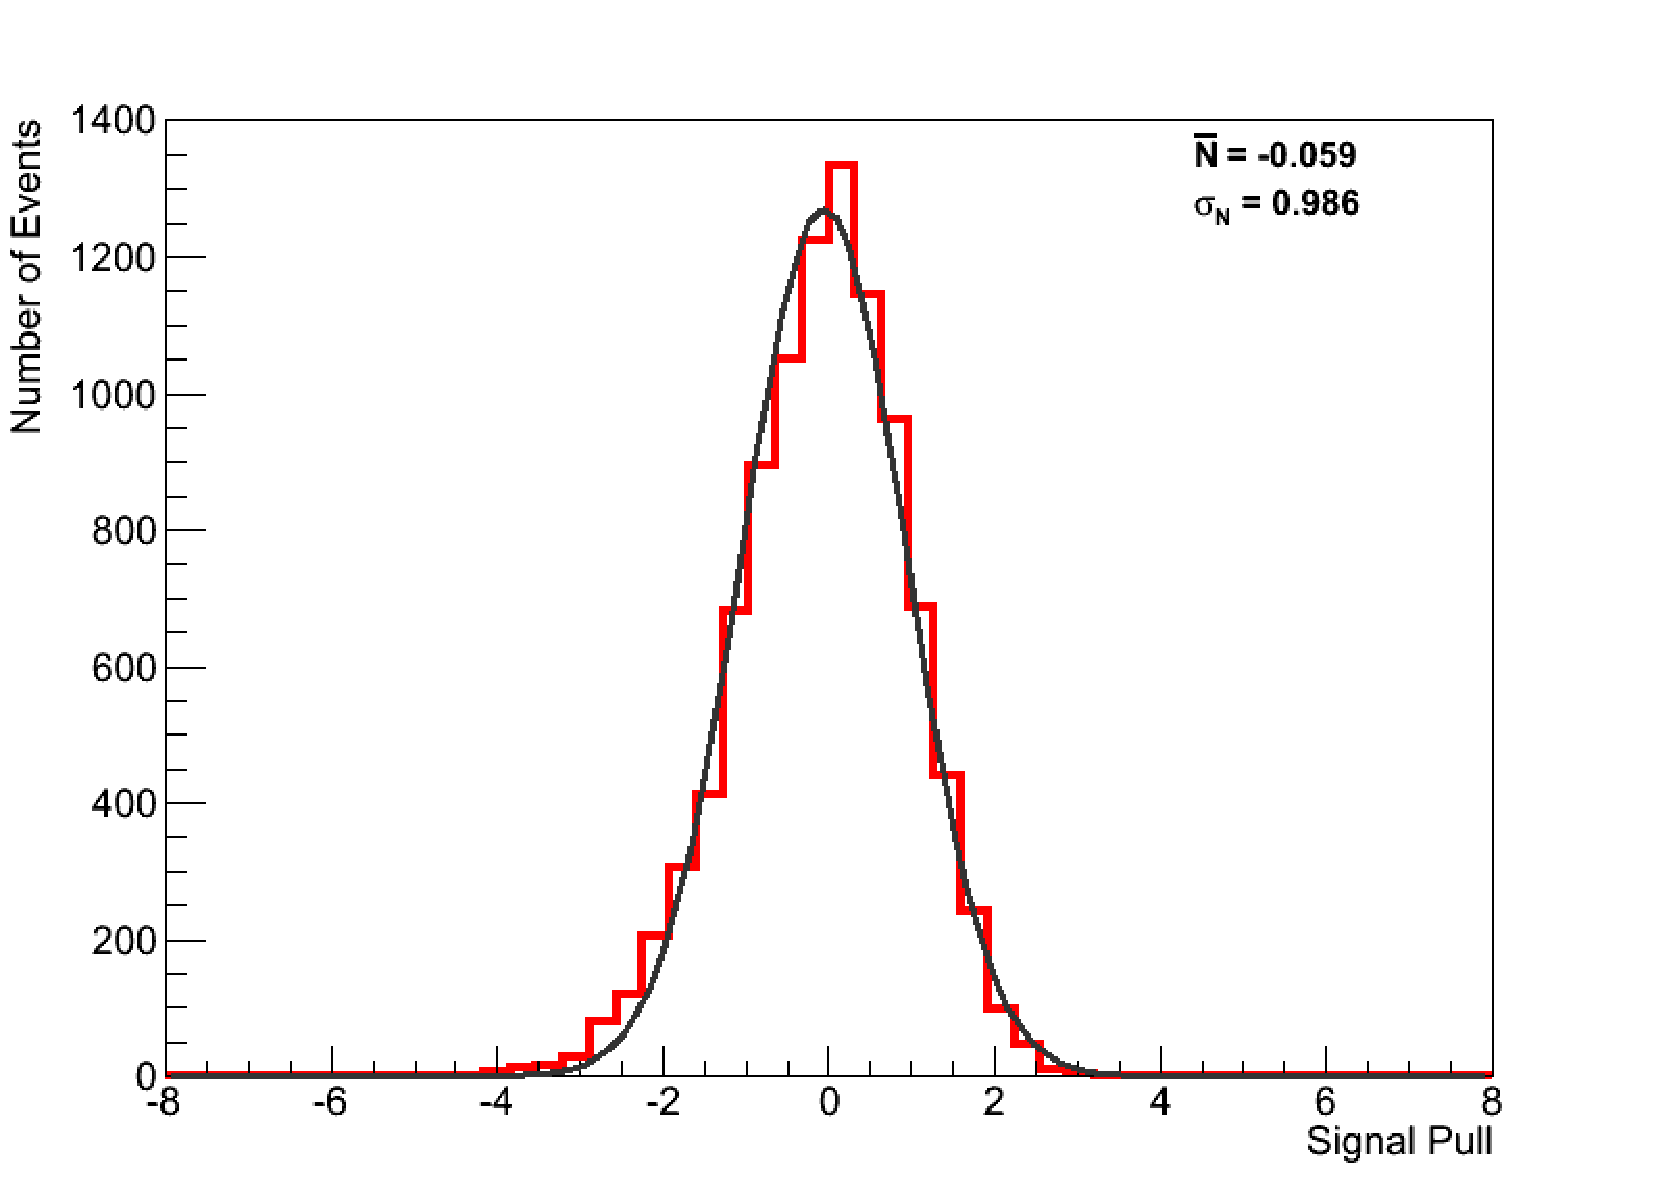
\includegraphics[width=0.45\textwidth]{figures/sigPullFitTwoD.pdf}
  %\includegraphics[width=0.45\textwidth]{figures/relativeErrFitTwoD.pdf}
  \caption{Pull distribution and Gaussian fit for 10,000 two dimensional toy MC experiments.}
  \label{fig:twoDpullPlot}
\end{figure}



\begin{table}[!ht]
\begin{center} 
\begin{tabular}{|c|c|}
\hline 
Analysis Method                 &  Relative Uncertainty on Signal Yield \\  \hline
Cut-Based Analysis (Scheme1)    &  XX\%                                 \\  
1D Fit to $m_{bb}$              &  XX\%                                 \\  
2D Fit                          &  XX\%                                 \\  \hline
\end{tabular}
\caption{Average Relative Uncertainty on Signal Yield for various analysis methods. }
\label{tab:RelativeUncertaintyOnSignalYield}
\end{center}
\end{table}
 

\section{Systematic Uncertainties}
\label{sec:systematics}



\section{Conclusion}
\label{sec:conclusion}




%===================================================================================================
%\clearpage

\vspace*{-0.2cm}
\thebibliography{12}

\bibitem{Item1}
 

%===================================================================================================

\appendix
\appendixpage




\end{document}
